\documentclass[twoside]{book}

% Packages required by doxygen
\usepackage{fixltx2e}
\usepackage{calc}
\usepackage{doxygen}
\usepackage[export]{adjustbox} % also loads graphicx
\usepackage{graphicx}
\usepackage[utf8]{inputenc}
\usepackage{makeidx}
\usepackage{multicol}
\usepackage{multirow}
\PassOptionsToPackage{warn}{textcomp}
\usepackage{textcomp}
\usepackage[nointegrals]{wasysym}
\usepackage[table]{xcolor}

% Font selection
\usepackage[T1]{fontenc}
\usepackage[scaled=.90]{helvet}
\usepackage{courier}
\usepackage{amssymb}
\usepackage{sectsty}
\renewcommand{\familydefault}{\sfdefault}
\allsectionsfont{%
  \fontseries{bc}\selectfont%
  \color{darkgray}%
}
\renewcommand{\DoxyLabelFont}{%
  \fontseries{bc}\selectfont%
  \color{darkgray}%
}
\newcommand{\+}{\discretionary{\mbox{\scriptsize$\hookleftarrow$}}{}{}}

% Page & text layout
\usepackage{geometry}
\geometry{%
  a4paper,%
  top=2.5cm,%
  bottom=2.5cm,%
  left=2.5cm,%
  right=2.5cm%
}
\tolerance=750
\hfuzz=15pt
\hbadness=750
\setlength{\emergencystretch}{15pt}
\setlength{\parindent}{0cm}
\setlength{\parskip}{0.2cm}
\makeatletter
\renewcommand{\paragraph}{%
  \@startsection{paragraph}{4}{0ex}{-1.0ex}{1.0ex}{%
    \normalfont\normalsize\bfseries\SS@parafont%
  }%
}
\renewcommand{\subparagraph}{%
  \@startsection{subparagraph}{5}{0ex}{-1.0ex}{1.0ex}{%
    \normalfont\normalsize\bfseries\SS@subparafont%
  }%
}
\makeatother

% Headers & footers
\usepackage{fancyhdr}
\pagestyle{fancyplain}
\fancyhead[LE]{\fancyplain{}{\bfseries\thepage}}
\fancyhead[CE]{\fancyplain{}{}}
\fancyhead[RE]{\fancyplain{}{\bfseries\leftmark}}
\fancyhead[LO]{\fancyplain{}{\bfseries\rightmark}}
\fancyhead[CO]{\fancyplain{}{}}
\fancyhead[RO]{\fancyplain{}{\bfseries\thepage}}
\fancyfoot[LE]{\fancyplain{}{}}
\fancyfoot[CE]{\fancyplain{}{}}
\fancyfoot[RE]{\fancyplain{}{\bfseries\scriptsize Generated on Tue Dec 22 2015 00\+:58\+:52 for whatsapl by Doxygen }}
\fancyfoot[LO]{\fancyplain{}{\bfseries\scriptsize Generated on Tue Dec 22 2015 00\+:58\+:52 for whatsapl by Doxygen }}
\fancyfoot[CO]{\fancyplain{}{}}
\fancyfoot[RO]{\fancyplain{}{}}
\renewcommand{\footrulewidth}{0.4pt}
\renewcommand{\chaptermark}[1]{%
  \markboth{#1}{}%
}
\renewcommand{\sectionmark}[1]{%
  \markright{\thesection\ #1}%
}

% Indices & bibliography
\usepackage{natbib}
\usepackage[titles]{tocloft}
\setcounter{tocdepth}{3}
\setcounter{secnumdepth}{5}
\makeindex

% Hyperlinks (required, but should be loaded last)
\usepackage{ifpdf}
\ifpdf
  \usepackage[pdftex,pagebackref=true]{hyperref}
\else
  \usepackage[ps2pdf,pagebackref=true]{hyperref}
\fi
\hypersetup{%
  colorlinks=true,%
  linkcolor=blue,%
  citecolor=blue,%
  unicode%
}

% Custom commands
\newcommand{\clearemptydoublepage}{%
  \newpage{\pagestyle{empty}\cleardoublepage}%
}


%===== C O N T E N T S =====

\begin{document}

% Titlepage & ToC
\hypersetup{pageanchor=false,
             bookmarks=true,
             bookmarksnumbered=true,
             pdfencoding=unicode
            }
\pagenumbering{roman}
\begin{titlepage}
\vspace*{7cm}
\begin{center}%
{\Large whatsapl }\\
\vspace*{1cm}
{\large Generated by Doxygen 1.8.10}\\
\vspace*{0.5cm}
{\small Tue Dec 22 2015 00:58:52}\\
\end{center}
\end{titlepage}
\clearemptydoublepage
\tableofcontents
\clearemptydoublepage
\pagenumbering{arabic}
\hypersetup{pageanchor=true}

%--- Begin generated contents ---
\chapter{Hierarchical Index}
\section{Class Hierarchy}
This inheritance list is sorted roughly, but not completely, alphabetically\+:\begin{DoxyCompactList}
\item \contentsline{section}{Amigo\+Inexistente}{\pageref{class_amigo_inexistente}}{}
\item \contentsline{section}{Amigo\+Ja\+Existe}{\pageref{class_amigo_ja_existe}}{}
\item \contentsline{section}{Bloqueado}{\pageref{class_bloqueado}}{}
\item \contentsline{section}{Comunidade}{\pageref{class_comunidade}}{}
\item \contentsline{section}{Conversa}{\pageref{class_conversa}}{}
\item \contentsline{section}{Data}{\pageref{class_data}}{}
\item \contentsline{section}{Data\+Invalida}{\pageref{class_data_invalida}}{}
\item \contentsline{section}{Grupo}{\pageref{class_grupo}}{}
\item \contentsline{section}{Grupo\+Inexistente}{\pageref{class_grupo_inexistente}}{}
\item \contentsline{section}{Hora\+Invalida}{\pageref{class_hora_invalida}}{}
\item \contentsline{section}{Hora\+Nova}{\pageref{class_hora_nova}}{}
\item \contentsline{section}{Horas}{\pageref{class_horas}}{}
\item \contentsline{section}{Idade\+Insuficiente}{\pageref{class_idade_insuficiente}}{}
\item \contentsline{section}{Input\+Fail}{\pageref{class_input_fail}}{}
\item \contentsline{section}{Membro}{\pageref{class_membro}}{}
\item \contentsline{section}{Membro\+Inexistente}{\pageref{class_membro_inexistente}}{}
\item \contentsline{section}{Mensagem}{\pageref{class_mensagem}}{}
\begin{DoxyCompactList}
\item \contentsline{section}{Msg\+Imagem}{\pageref{class_msg_imagem}}{}
\item \contentsline{section}{Msg\+Texto}{\pageref{class_msg_texto}}{}
\item \contentsline{section}{Msg\+Video}{\pageref{class_msg_video}}{}
\end{DoxyCompactList}
\item \contentsline{section}{Nao\+Moderador}{\pageref{class_nao_moderador}}{}
\item \contentsline{section}{Nao\+Participante}{\pageref{class_nao_participante}}{}
\item \contentsline{section}{Opccao\+Invalida$<$ N $>$}{\pageref{class_opccao_invalida}}{}
\item \contentsline{section}{Pedido\+Inexistente}{\pageref{class_pedido_inexistente}}{}
\item \contentsline{section}{Utilizador}{\pageref{class_utilizador}}{}
\item \contentsline{section}{Utilizador\+Inexistente}{\pageref{class_utilizador_inexistente}}{}
\item \contentsline{section}{Utilizador\+Ja\+Existe}{\pageref{class_utilizador_ja_existe}}{}
\item \contentsline{section}{Voltar\+Atras}{\pageref{class_voltar_atras}}{}
\end{DoxyCompactList}

\chapter{Class Index}
\section{Class List}
Here are the classes, structs, unions and interfaces with brief descriptions\+:\begin{DoxyCompactList}
\item\contentsline{section}{\hyperlink{class_amigo_inexistente}{Amigo\+Inexistente} \\*Classe que representa uma excecao da classe utilizador. Esta excecao e lancada quando o amigo do utilizador nao existe }{\pageref{class_amigo_inexistente}}{}
\item\contentsline{section}{\hyperlink{class_amigo_ja_existe}{Amigo\+Ja\+Existe} \\*Classe que representa uma excecao da classe utilizador. Esta excecao e lancada quando o amigo do utilizador ja existe }{\pageref{class_amigo_ja_existe}}{}
\item\contentsline{section}{\hyperlink{class_bloqueado}{Bloqueado} \\*Classe que representa uma excecao da classe grupo. Esta excecao e lancada quando um utilizador que foi bloqueado de um grupo tenta enviar uma mensagem }{\pageref{class_bloqueado}}{}
\item\contentsline{section}{\hyperlink{class_comunidade}{Comunidade} \\*Classe \hyperlink{class_comunidade}{Comunidade}. Class que contem e gere todos os utilizadores E possivel ordenar os utilizadores por data de ades�o, login }{\pageref{class_comunidade}}{}
\item\contentsline{section}{\hyperlink{class_conversa}{Conversa} }{\pageref{class_conversa}}{}
\item\contentsline{section}{\hyperlink{class_data}{Data} \\*Classe \hyperlink{class_data}{Data}. Classe que indica as data (dia mes e ano) ao utilizador. E possivel modificar a data }{\pageref{class_data}}{}
\item\contentsline{section}{\hyperlink{class_data_invalida}{Data\+Invalida} \\*Classe \hyperlink{class_data_invalida}{Data\+Invalida}. E uma classe que indica uma execao da classe \hyperlink{class_data}{Data} }{\pageref{class_data_invalida}}{}
\item\contentsline{section}{\hyperlink{class_grupo}{Grupo} \\*Classe \hyperlink{class_grupo}{Grupo}. Classe que forma um grupo. Um grupo pode ter varios membros, mas apenas um moderador. O moderador e o utilizador que gere o grupo\+: permite aceitar pedidos de adesao ao grupo, retirar, bloquear ou desbloquear elementos, Um grupo tem um titulo e uma data de criacao. O utilizador moderador e o utilizador que cria o grupo, logo contem a mesma data de adesao que a data de criacao do grupo. Um grupo contem uma unica conversa que contem todos os utilizadores. No entanto podem estar bloqueados, pelo que nao podem enviar mensagens }{\pageref{class_grupo}}{}
\item\contentsline{section}{\hyperlink{class_grupo_inexistente}{Grupo\+Inexistente} \\*Classe excep��o que � lan�ada quando se procura um grupo que nao existe }{\pageref{class_grupo_inexistente}}{}
\item\contentsline{section}{\hyperlink{class_hora_invalida}{Hora\+Invalida} \\*Classe \hyperlink{class_hora_invalida}{Hora\+Invalida}. E uma classe que indica uma execao da classe \hyperlink{class_horas}{Horas} }{\pageref{class_hora_invalida}}{}
\item\contentsline{section}{\hyperlink{class_hora_nova}{Hora\+Nova} }{\pageref{class_hora_nova}}{}
\item\contentsline{section}{\hyperlink{class_horas}{Horas} \\*Classe \hyperlink{class_horas}{Horas}. Classe que indica as horas (hora e minuto) ao utilizador. E possivel modificar as horas }{\pageref{class_horas}}{}
\item\contentsline{section}{\hyperlink{class_idade_insuficiente}{Idade\+Insuficiente} \\*Classe que representa uma excecao da classe utilizador. Esta excecao e lancada quando um utilizador nao tem idade suficiente para se registar na aplica��o }{\pageref{class_idade_insuficiente}}{}
\item\contentsline{section}{\hyperlink{class_input_fail}{Input\+Fail} \\*Classe que representa uma excecao da classe main. Impede que o programa aborte quando sao introduzidos valores errados no buffer }{\pageref{class_input_fail}}{}
\item\contentsline{section}{\hyperlink{class_membro}{Membro} \\*Classe \hyperlink{class_membro}{Membro}. Classe que define os parametros necessarios para um utilizador estar num grupo. Associa o login de um utilizador a data de adesao no grupo e a um boleano que indica se esta bloqueado }{\pageref{class_membro}}{}
\item\contentsline{section}{\hyperlink{class_membro_inexistente}{Membro\+Inexistente} \\*Classe que representa uma excecao da classe grupo. Esta excecao e lancada no caso de n�o haver um membro com um determinado login }{\pageref{class_membro_inexistente}}{}
\item\contentsline{section}{\hyperlink{class_mensagem}{Mensagem} }{\pageref{class_mensagem}}{}
\item\contentsline{section}{\hyperlink{class_msg_imagem}{Msg\+Imagem} }{\pageref{class_msg_imagem}}{}
\item\contentsline{section}{\hyperlink{class_msg_texto}{Msg\+Texto} }{\pageref{class_msg_texto}}{}
\item\contentsline{section}{\hyperlink{class_msg_video}{Msg\+Video} }{\pageref{class_msg_video}}{}
\item\contentsline{section}{\hyperlink{class_nao_moderador}{Nao\+Moderador} \\*Classe que representa uma excecao da classe grupo. Esta excecao e lancada no caso de o utilizador que esta a pedir permissoes nao ser o utilizador moderador do grupo }{\pageref{class_nao_moderador}}{}
\item\contentsline{section}{\hyperlink{class_nao_participante}{Nao\+Participante} \\*Classe que representa uma excecao da classe conversa. Esta excecao e lancada quando um utilizador que nao participa na conversa tenta enviar mensagens }{\pageref{class_nao_participante}}{}
\item\contentsline{section}{\hyperlink{class_opccao_invalida}{Opccao\+Invalida$<$ N $>$} \\*Classe que representa uma excecao da classe Main. Esta excecao e lancada quando a opcao colocada nao esta entre os limites estabelecidos. E uma classe template pois pode receber mais que um tipo de dados }{\pageref{class_opccao_invalida}}{}
\item\contentsline{section}{\hyperlink{class_pedido_inexistente}{Pedido\+Inexistente} \\*Classe que representa uma excecao da classe grupo. Esta excecao e lancada quando nao existe no vetor de pedidos de adesao de um grupo o login recebido }{\pageref{class_pedido_inexistente}}{}
\item\contentsline{section}{\hyperlink{class_utilizador}{Utilizador} }{\pageref{class_utilizador}}{}
\item\contentsline{section}{\hyperlink{class_utilizador_inexistente}{Utilizador\+Inexistente} \\*Classe que representa uma excecao da classe utilizador. Esta excecao e lan�ada quando um utilizador n�o existe }{\pageref{class_utilizador_inexistente}}{}
\item\contentsline{section}{\hyperlink{class_utilizador_ja_existe}{Utilizador\+Ja\+Existe} \\*Classe que representa uma excecao da classe utilizador. Esta excecao e lancada quando um utilizador ja existe e nao devia }{\pageref{class_utilizador_ja_existe}}{}
\item\contentsline{section}{\hyperlink{class_voltar_atras}{Voltar\+Atras} \\*Classe que representa uma excecao da classe main. Permite ter a opcao de voltar a tras nos menus }{\pageref{class_voltar_atras}}{}
\end{DoxyCompactList}

\chapter{Class Documentation}
\hypertarget{class_amigo_inexistente}{}\section{Amigo\+Inexistente Class Reference}
\label{class_amigo_inexistente}\index{Amigo\+Inexistente@{Amigo\+Inexistente}}


Classe que representa uma excecao da classe utilizador. Esta excecao e lancada quando o amigo do utilizador nao existe.  




{\ttfamily \#include $<$Excecoes.\+h$>$}

\subsection*{Public Member Functions}
\begin{DoxyCompactItemize}
\item 
\hyperlink{class_amigo_inexistente_a214d9d7a9579e42d67f8c7fe290958f3}{Amigo\+Inexistente} (string l)
\begin{DoxyCompactList}\small\item\em Construtor. Inicializa o membro login com o login do amigo do utilizador. \end{DoxyCompactList}\item 
string \hyperlink{class_amigo_inexistente_a72d6ea60bacc6a8deacefc1f130ce883}{get\+Login} () const 
\begin{DoxyCompactList}\small\item\em Funcao que retorna o login do utilizador que criou a excecao. \end{DoxyCompactList}\end{DoxyCompactItemize}


\subsection{Detailed Description}
Classe que representa uma excecao da classe utilizador. Esta excecao e lancada quando o amigo do utilizador nao existe. 

\subsection{Constructor \& Destructor Documentation}
\hypertarget{class_amigo_inexistente_a214d9d7a9579e42d67f8c7fe290958f3}{}\index{Amigo\+Inexistente@{Amigo\+Inexistente}!Amigo\+Inexistente@{Amigo\+Inexistente}}
\index{Amigo\+Inexistente@{Amigo\+Inexistente}!Amigo\+Inexistente@{Amigo\+Inexistente}}
\subsubsection[{Amigo\+Inexistente(string l)}]{\setlength{\rightskip}{0pt plus 5cm}Amigo\+Inexistente\+::\+Amigo\+Inexistente (
\begin{DoxyParamCaption}
\item[{string}]{l}
\end{DoxyParamCaption}
)\hspace{0.3cm}{\ttfamily [inline]}}\label{class_amigo_inexistente_a214d9d7a9579e42d67f8c7fe290958f3}


Construtor. Inicializa o membro login com o login do amigo do utilizador. 


\begin{DoxyParams}{Parameters}
{\em l} & Login do amigo do utilizador recebido. \\
\hline
\end{DoxyParams}


\subsection{Member Function Documentation}
\hypertarget{class_amigo_inexistente_a72d6ea60bacc6a8deacefc1f130ce883}{}\index{Amigo\+Inexistente@{Amigo\+Inexistente}!get\+Login@{get\+Login}}
\index{get\+Login@{get\+Login}!Amigo\+Inexistente@{Amigo\+Inexistente}}
\subsubsection[{get\+Login() const }]{\setlength{\rightskip}{0pt plus 5cm}string Amigo\+Inexistente\+::get\+Login (
\begin{DoxyParamCaption}
{}
\end{DoxyParamCaption}
) const\hspace{0.3cm}{\ttfamily [inline]}}\label{class_amigo_inexistente_a72d6ea60bacc6a8deacefc1f130ce883}


Funcao que retorna o login do utilizador que criou a excecao. 

\begin{DoxyReturn}{Returns}
Login do utilizador. 
\end{DoxyReturn}


The documentation for this class was generated from the following file\+:\begin{DoxyCompactItemize}
\item 
Excecoes.\+h\end{DoxyCompactItemize}

\hypertarget{class_amigo_ja_existe}{}\section{Amigo\+Ja\+Existe Class Reference}
\label{class_amigo_ja_existe}\index{Amigo\+Ja\+Existe@{Amigo\+Ja\+Existe}}
\subsection*{Public Member Functions}
\begin{DoxyCompactItemize}
\item 
\hypertarget{class_amigo_ja_existe_a9ed8e09fdd1560f9ebf3139dafe45ffe}{}{\bfseries Amigo\+Ja\+Existe} (\hyperlink{class_utilizador}{Utilizador} u)\label{class_amigo_ja_existe_a9ed8e09fdd1560f9ebf3139dafe45ffe}

\end{DoxyCompactItemize}


The documentation for this class was generated from the following file\+:\begin{DoxyCompactItemize}
\item 
\hyperlink{_utilizador_8h}{Utilizador.\+h}\end{DoxyCompactItemize}

\hypertarget{class_binary_node}{}\section{Binary\+Node$<$ Comparable $>$ Class Template Reference}
\label{class_binary_node}\index{Binary\+Node$<$ Comparable $>$@{Binary\+Node$<$ Comparable $>$}}
\subsection*{Friends}
\begin{DoxyCompactItemize}
\item 
\hypertarget{class_binary_node_a28a1adb9906f3ff7e12c2cb6fa2bd54e}{}class {\bfseries B\+S\+T$<$ Comparable $>$}\label{class_binary_node_a28a1adb9906f3ff7e12c2cb6fa2bd54e}

\item 
\hypertarget{class_binary_node_aab3993acac2ab24a0b59edb0c3acc775}{}class {\bfseries B\+S\+T\+Itr\+In$<$ Comparable $>$}\label{class_binary_node_aab3993acac2ab24a0b59edb0c3acc775}

\item 
\hypertarget{class_binary_node_a45a55df6f11541416d4ea7684c575c1a}{}class {\bfseries B\+S\+T\+Itr\+Pre$<$ Comparable $>$}\label{class_binary_node_a45a55df6f11541416d4ea7684c575c1a}

\item 
\hypertarget{class_binary_node_a5dc153694be266f6e772659486219da7}{}class {\bfseries B\+S\+T\+Itr\+Post$<$ Comparable $>$}\label{class_binary_node_a5dc153694be266f6e772659486219da7}

\item 
\hypertarget{class_binary_node_a26ff00bc0d87069aed877f10fd3c80a8}{}class {\bfseries B\+S\+T\+Itr\+Level$<$ Comparable $>$}\label{class_binary_node_a26ff00bc0d87069aed877f10fd3c80a8}

\end{DoxyCompactItemize}


The documentation for this class was generated from the following file\+:\begin{DoxyCompactItemize}
\item 
B\+S\+T.\+h\end{DoxyCompactItemize}

\hypertarget{class_bloqueado}{}\section{Bloqueado Class Reference}
\label{class_bloqueado}\index{Bloqueado@{Bloqueado}}


Classe que representa uma excecao da classe grupo. Esta excecao e lancada quando um utilizador que foi bloqueado de um grupo tenta enviar uma mensagem.  




{\ttfamily \#include $<$Excecoes.\+h$>$}

\subsection*{Public Member Functions}
\begin{DoxyCompactItemize}
\item 
\hyperlink{class_bloqueado_aeed14705a1258de654aa8017418f9da4}{Bloqueado} (string l)
\begin{DoxyCompactList}\small\item\em Construtor. Inicializa o membro login com o login recebido. \end{DoxyCompactList}\item 
\hypertarget{class_bloqueado_a4be9531006bc7b1ca77c9c9dbe5789a7}{}string \hyperlink{class_bloqueado_a4be9531006bc7b1ca77c9c9dbe5789a7}{get\+Login} () const \label{class_bloqueado_a4be9531006bc7b1ca77c9c9dbe5789a7}

\begin{DoxyCompactList}\small\item\em Funcao que retorna o login do utilizador que retorna a excecao. \end{DoxyCompactList}\end{DoxyCompactItemize}


\subsection{Detailed Description}
Classe que representa uma excecao da classe grupo. Esta excecao e lancada quando um utilizador que foi bloqueado de um grupo tenta enviar uma mensagem. 

\subsection{Constructor \& Destructor Documentation}
\hypertarget{class_bloqueado_aeed14705a1258de654aa8017418f9da4}{}\index{Bloqueado@{Bloqueado}!Bloqueado@{Bloqueado}}
\index{Bloqueado@{Bloqueado}!Bloqueado@{Bloqueado}}
\subsubsection[{Bloqueado(string l)}]{\setlength{\rightskip}{0pt plus 5cm}Bloqueado\+::\+Bloqueado (
\begin{DoxyParamCaption}
\item[{string}]{l}
\end{DoxyParamCaption}
)\hspace{0.3cm}{\ttfamily [inline]}}\label{class_bloqueado_aeed14705a1258de654aa8017418f9da4}


Construtor. Inicializa o membro login com o login recebido. 


\begin{DoxyParams}{Parameters}
{\em l} & Login recebido. \\
\hline
\end{DoxyParams}


The documentation for this class was generated from the following file\+:\begin{DoxyCompactItemize}
\item 
Excecoes.\+h\end{DoxyCompactItemize}

\hypertarget{class_b_s_t}{}\section{B\+S\+T$<$ Comparable $>$ Class Template Reference}
\label{class_b_s_t}\index{B\+S\+T$<$ Comparable $>$@{B\+S\+T$<$ Comparable $>$}}
\subsection*{Public Member Functions}
\begin{DoxyCompactItemize}
\item 
\hypertarget{class_b_s_t_a3185a79cf472271f122a97d0f59022d1}{}{\bfseries B\+S\+T} (const Comparable \&not\+Found)\label{class_b_s_t_a3185a79cf472271f122a97d0f59022d1}

\item 
\hypertarget{class_b_s_t_a163232cc6ffcbd1a51707efcc3fa36ca}{}{\bfseries B\+S\+T} (const \hyperlink{class_b_s_t}{B\+S\+T} \&rhs)\label{class_b_s_t_a163232cc6ffcbd1a51707efcc3fa36ca}

\item 
\hypertarget{class_b_s_t_a34fd17be76f49a77573185f29dede6be}{}const Comparable \& {\bfseries find\+Min} () const \label{class_b_s_t_a34fd17be76f49a77573185f29dede6be}

\item 
\hypertarget{class_b_s_t_aee725fe273c0b3641070883b50eee271}{}const Comparable \& {\bfseries find\+Max} () const \label{class_b_s_t_aee725fe273c0b3641070883b50eee271}

\item 
\hypertarget{class_b_s_t_a337dce7f94a881e253635cbf3ac7eacf}{}const Comparable \& {\bfseries find} (const Comparable \&x) const \label{class_b_s_t_a337dce7f94a881e253635cbf3ac7eacf}

\item 
\hypertarget{class_b_s_t_a8018fc7d6c15b2564c10ddcc4316c64d}{}bool {\bfseries is\+Empty} () const \label{class_b_s_t_a8018fc7d6c15b2564c10ddcc4316c64d}

\item 
\hypertarget{class_b_s_t_a5270473db9e17e1737b92dd0d6cd0ee5}{}void {\bfseries print\+Tree} () const \label{class_b_s_t_a5270473db9e17e1737b92dd0d6cd0ee5}

\item 
\hypertarget{class_b_s_t_a050d829503a88714c4ad0773cf6d3af6}{}void {\bfseries make\+Empty} ()\label{class_b_s_t_a050d829503a88714c4ad0773cf6d3af6}

\item 
\hypertarget{class_b_s_t_a2b117df6521c7d61dac75ff2c938bae7}{}void {\bfseries insert} (const Comparable \&x)\label{class_b_s_t_a2b117df6521c7d61dac75ff2c938bae7}

\item 
\hypertarget{class_b_s_t_a6f01a0b44daf82a42022b6eb4c0df7a2}{}void {\bfseries remove} (const Comparable \&x)\label{class_b_s_t_a6f01a0b44daf82a42022b6eb4c0df7a2}

\item 
\hypertarget{class_b_s_t_aa80c39f454c89d4a202be3d1445823f3}{}const \hyperlink{class_b_s_t}{B\+S\+T} \& {\bfseries operator=} (const \hyperlink{class_b_s_t}{B\+S\+T} \&rhs)\label{class_b_s_t_aa80c39f454c89d4a202be3d1445823f3}

\end{DoxyCompactItemize}
\subsection*{Friends}
\begin{DoxyCompactItemize}
\item 
\hypertarget{class_b_s_t_aab3993acac2ab24a0b59edb0c3acc775}{}class {\bfseries B\+S\+T\+Itr\+In$<$ Comparable $>$}\label{class_b_s_t_aab3993acac2ab24a0b59edb0c3acc775}

\item 
\hypertarget{class_b_s_t_a45a55df6f11541416d4ea7684c575c1a}{}class {\bfseries B\+S\+T\+Itr\+Pre$<$ Comparable $>$}\label{class_b_s_t_a45a55df6f11541416d4ea7684c575c1a}

\item 
\hypertarget{class_b_s_t_a5dc153694be266f6e772659486219da7}{}class {\bfseries B\+S\+T\+Itr\+Post$<$ Comparable $>$}\label{class_b_s_t_a5dc153694be266f6e772659486219da7}

\item 
\hypertarget{class_b_s_t_a26ff00bc0d87069aed877f10fd3c80a8}{}class {\bfseries B\+S\+T\+Itr\+Level$<$ Comparable $>$}\label{class_b_s_t_a26ff00bc0d87069aed877f10fd3c80a8}

\end{DoxyCompactItemize}


The documentation for this class was generated from the following file\+:\begin{DoxyCompactItemize}
\item 
B\+S\+T.\+h\end{DoxyCompactItemize}

\hypertarget{class_b_s_t_itr_in}{}\section{B\+S\+T\+Itr\+In$<$ Comparable $>$ Class Template Reference}
\label{class_b_s_t_itr_in}\index{B\+S\+T\+Itr\+In$<$ Comparable $>$@{B\+S\+T\+Itr\+In$<$ Comparable $>$}}
\subsection*{Public Member Functions}
\begin{DoxyCompactItemize}
\item 
\hypertarget{class_b_s_t_itr_in_ac836e2f560fed9cc7ef8e5431a2836cc}{}{\bfseries B\+S\+T\+Itr\+In} (const \hyperlink{class_b_s_t}{B\+S\+T}$<$ Comparable $>$ \&bt)\label{class_b_s_t_itr_in_ac836e2f560fed9cc7ef8e5431a2836cc}

\item 
\hypertarget{class_b_s_t_itr_in_ac772d3ebbac748c5f8cf9bc659f2e32c}{}void {\bfseries advance} ()\label{class_b_s_t_itr_in_ac772d3ebbac748c5f8cf9bc659f2e32c}

\item 
\hypertarget{class_b_s_t_itr_in_ac7ac215c1247bd25fc1fdb8053826a32}{}Comparable \& {\bfseries retrieve} ()\label{class_b_s_t_itr_in_ac7ac215c1247bd25fc1fdb8053826a32}

\item 
\hypertarget{class_b_s_t_itr_in_a6f9a43217862c263a9bf15b9a08b889a}{}bool {\bfseries is\+At\+End} ()\label{class_b_s_t_itr_in_a6f9a43217862c263a9bf15b9a08b889a}

\end{DoxyCompactItemize}


The documentation for this class was generated from the following file\+:\begin{DoxyCompactItemize}
\item 
B\+S\+T.\+h\end{DoxyCompactItemize}

\hypertarget{class_b_s_t_itr_level}{}\section{B\+S\+T\+Itr\+Level$<$ Comparable $>$ Class Template Reference}
\label{class_b_s_t_itr_level}\index{B\+S\+T\+Itr\+Level$<$ Comparable $>$@{B\+S\+T\+Itr\+Level$<$ Comparable $>$}}
\subsection*{Public Member Functions}
\begin{DoxyCompactItemize}
\item 
\hypertarget{class_b_s_t_itr_level_a8fd5cdde93eb182c4cd5cf6b2c5efaeb}{}{\bfseries B\+S\+T\+Itr\+Level} (const \hyperlink{class_b_s_t}{B\+S\+T}$<$ Comparable $>$ \&bt)\label{class_b_s_t_itr_level_a8fd5cdde93eb182c4cd5cf6b2c5efaeb}

\item 
\hypertarget{class_b_s_t_itr_level_ad54a6fa289a59d6050b507abe40d463b}{}void {\bfseries advance} ()\label{class_b_s_t_itr_level_ad54a6fa289a59d6050b507abe40d463b}

\item 
\hypertarget{class_b_s_t_itr_level_a0340bd9f21f72ae25348f383e67e7f91}{}Comparable \& {\bfseries retrieve} ()\label{class_b_s_t_itr_level_a0340bd9f21f72ae25348f383e67e7f91}

\item 
\hypertarget{class_b_s_t_itr_level_a89bc8e81dde255fd6bad917cacc0d489}{}bool {\bfseries is\+At\+End} ()\label{class_b_s_t_itr_level_a89bc8e81dde255fd6bad917cacc0d489}

\end{DoxyCompactItemize}


The documentation for this class was generated from the following file\+:\begin{DoxyCompactItemize}
\item 
B\+S\+T.\+h\end{DoxyCompactItemize}

\hypertarget{class_b_s_t_itr_post}{}\section{B\+S\+T\+Itr\+Post$<$ Comparable $>$ Class Template Reference}
\label{class_b_s_t_itr_post}\index{B\+S\+T\+Itr\+Post$<$ Comparable $>$@{B\+S\+T\+Itr\+Post$<$ Comparable $>$}}
\subsection*{Public Member Functions}
\begin{DoxyCompactItemize}
\item 
\hypertarget{class_b_s_t_itr_post_acf7e537dea01978f40c40909c55c56c2}{}{\bfseries B\+S\+T\+Itr\+Post} (const \hyperlink{class_b_s_t}{B\+S\+T}$<$ Comparable $>$ \&bt)\label{class_b_s_t_itr_post_acf7e537dea01978f40c40909c55c56c2}

\item 
\hypertarget{class_b_s_t_itr_post_a376098e5a82cd02118dd4dcdec49bb26}{}void {\bfseries advance} ()\label{class_b_s_t_itr_post_a376098e5a82cd02118dd4dcdec49bb26}

\item 
\hypertarget{class_b_s_t_itr_post_a72446e4d0df0bcafc14294a78faeb56e}{}Comparable \& {\bfseries retrieve} ()\label{class_b_s_t_itr_post_a72446e4d0df0bcafc14294a78faeb56e}

\item 
\hypertarget{class_b_s_t_itr_post_a2f330e73bb817e8bd1c797805e66ddb7}{}bool {\bfseries is\+At\+End} ()\label{class_b_s_t_itr_post_a2f330e73bb817e8bd1c797805e66ddb7}

\end{DoxyCompactItemize}


The documentation for this class was generated from the following file\+:\begin{DoxyCompactItemize}
\item 
B\+S\+T.\+h\end{DoxyCompactItemize}

\hypertarget{class_b_s_t_itr_pre}{}\section{B\+S\+T\+Itr\+Pre$<$ Comparable $>$ Class Template Reference}
\label{class_b_s_t_itr_pre}\index{B\+S\+T\+Itr\+Pre$<$ Comparable $>$@{B\+S\+T\+Itr\+Pre$<$ Comparable $>$}}
\subsection*{Public Member Functions}
\begin{DoxyCompactItemize}
\item 
\hypertarget{class_b_s_t_itr_pre_a11b1cd4e783f153b9c1b64ce2ec8077e}{}{\bfseries B\+S\+T\+Itr\+Pre} (const \hyperlink{class_b_s_t}{B\+S\+T}$<$ Comparable $>$ \&bt)\label{class_b_s_t_itr_pre_a11b1cd4e783f153b9c1b64ce2ec8077e}

\item 
\hypertarget{class_b_s_t_itr_pre_a7a743d66a842018fd833fb2b0737254d}{}void {\bfseries advance} ()\label{class_b_s_t_itr_pre_a7a743d66a842018fd833fb2b0737254d}

\item 
\hypertarget{class_b_s_t_itr_pre_af40033e97f63bf025c2e33a9fdce4c43}{}Comparable \& {\bfseries retrieve} ()\label{class_b_s_t_itr_pre_af40033e97f63bf025c2e33a9fdce4c43}

\item 
\hypertarget{class_b_s_t_itr_pre_ae282a7b9ffa9d250bb0f6a6d79f6e8d0}{}bool {\bfseries is\+At\+End} ()\label{class_b_s_t_itr_pre_ae282a7b9ffa9d250bb0f6a6d79f6e8d0}

\end{DoxyCompactItemize}


The documentation for this class was generated from the following file\+:\begin{DoxyCompactItemize}
\item 
B\+S\+T.\+h\end{DoxyCompactItemize}

\hypertarget{class_comunidade}{}\section{Comunidade Class Reference}
\label{class_comunidade}\index{Comunidade@{Comunidade}}


Classe \hyperlink{class_comunidade}{Comunidade}. Class que contem e gere todos os utilizadores E possivel ordenar os utilizadores por data de ades�o, login.  




{\ttfamily \#include $<$Comunidade.\+h$>$}

\subsection*{Public Member Functions}
\begin{DoxyCompactItemize}
\item 
\hypertarget{class_comunidade_ad44e0775322f253c3c28bae06bf844de}{}\hyperlink{class_comunidade_ad44e0775322f253c3c28bae06bf844de}{Comunidade} ()\label{class_comunidade_ad44e0775322f253c3c28bae06bf844de}

\begin{DoxyCompactList}\small\item\em Construtor Construtor default que inicializa o vector de utilizadores a zero. \end{DoxyCompactList}\item 
void \hyperlink{class_comunidade_a293d4cdbd618422869ef4d71c34cdb9f}{update\+Utilizadores\+Inativos} ()
\item 
void \hyperlink{class_comunidade_a6672ca4af496637a47f1c72e9b038a13}{print\+Utilizadores\+Inativos} () const 
\item 
int \hyperlink{class_comunidade_accf146332d17ad07080bcee3bb2a727c}{existe\+Util} (\hyperlink{class_utilizador}{Utilizador} $\ast$util) const 
\item 
int \hyperlink{class_comunidade_a467973e3790e6fdd832bb9702eb635bb}{existe\+Util\+Login} (string login) const 
\begin{DoxyCompactList}\small\item\em Funcao que procura um utilizador na comunidade pelo login. \end{DoxyCompactList}\item 
int \hyperlink{class_comunidade_a8c7188c4db52d049b25b158497ac8c14}{existe\+Util\+Nome} (string nome) const 
\item 
\hyperlink{class_grupo}{Grupo} $\ast$ \hyperlink{class_comunidade_adfc1f95d2fc409985c291bd29c9b7855}{existe\+Grupo} (string grupo) const 
\item 
\hyperlink{class_utilizador}{Utilizador} $\ast$ \hyperlink{class_comunidade_a4c537ae9c435a276154051da96e628af}{utilizador\+Na\+Posicao} (int pos) const 
\item 
void \hyperlink{class_comunidade_a1961b08389ea8fc40a7cdd099d733ad7}{adicionar\+Util} (\hyperlink{class_utilizador}{Utilizador} $\ast$util)
\item 
void \hyperlink{class_comunidade_a4770f5f57ce9e47e0a661b3b923061d8}{ordena\+Data} ()
\item 
void \hyperlink{class_comunidade_a80e54e2c6d1f2b6011453b5043860c82}{ordena\+Login} ()
\item 
void \hyperlink{class_comunidade_abcdd6a3eba7ff0c2c53e5ea024a98a46}{ver\+Utilizador} (\hyperlink{class_utilizador}{Utilizador} $\ast$util) const 
\item 
void \hyperlink{class_comunidade_ae7c4558f4f6174518b7e15ab007f04fd}{print\+Comunidade} () const 
\item 
bool \hyperlink{class_comunidade_a5455ec3855626919ba1b4d919e38132f}{existe\+Login} (string l) const 
\begin{DoxyCompactList}\small\item\em Funcao que verifica se existe um login. \end{DoxyCompactList}\item 
void \hyperlink{class_comunidade_a3a39cdd6a92e68d4d25e6b99b68da32d}{le\+Utilizador} (string path)
\begin{DoxyCompactList}\small\item\em Funcao que le um ficheiro de texto com os utilizadores e coloca a informacao no local certo. \end{DoxyCompactList}\item 
void \hyperlink{class_comunidade_ae9ed6b53c7fc25c1286dd8c0ff3d2ed3}{le\+Conversa} (string path)
\begin{DoxyCompactList}\small\item\em Funcao que le um ficheiro de texto com as conversas e coloca a informacao no local certo. \end{DoxyCompactList}\item 
void \hyperlink{class_comunidade_a6bdcfec2d0bd2f2d518713830fc17242}{le\+Grupo} (string path)
\begin{DoxyCompactList}\small\item\em Funcao que le um ficheiro de texto com os grupos e coloca a informacao no local certo. \end{DoxyCompactList}\item 
int \hyperlink{class_comunidade_a78e9b2f723065c9085dd8984cba6691f}{escreve\+Utilizador} (string path)
\begin{DoxyCompactList}\small\item\em Funcao que converte a informacao do programa sobre utilizadores num ficheiro .txt. \end{DoxyCompactList}\item 
int \hyperlink{class_comunidade_a0de7c5114b4754401b8e12e4ed0ba34e}{escreve\+Conversa} (string path)
\begin{DoxyCompactList}\small\item\em Funcao que converte a informacao do programa sobre conversas num ficheiro .txt. \end{DoxyCompactList}\item 
int \hyperlink{class_comunidade_aecb81c6a5dba43898876761c491db171}{escreve\+Grupo} (string path)
\begin{DoxyCompactList}\small\item\em Funcao que converte a informacao do programa sobre grupos num ficheiro .txt. \end{DoxyCompactList}\item 
\hyperlink{class_b_s_t}{B\+S\+T}$<$ \hyperlink{class_utilizador}{Utilizador} $>$ \hyperlink{class_comunidade_a0cbd33ffe5af96e358a3ca0856bcdd92}{top\+Utilizadores} () const 
\begin{DoxyCompactList}\small\item\em Funcao que analiza os utilizadores mais ativos nos ultimos 3 dias da aplica��o. \end{DoxyCompactList}\item 
\hypertarget{class_comunidade_adcb5e4a98d6e87b1cd531bc18f478484}{}void \hyperlink{class_comunidade_adcb5e4a98d6e87b1cd531bc18f478484}{display\+Top\+Utilizadores} () const \label{class_comunidade_adcb5e4a98d6e87b1cd531bc18f478484}

\begin{DoxyCompactList}\small\item\em Funcao que mostra no ecra os utilizadores mais ativos. \end{DoxyCompactList}\end{DoxyCompactItemize}


\subsection{Detailed Description}
Classe \hyperlink{class_comunidade}{Comunidade}. Class que contem e gere todos os utilizadores E possivel ordenar os utilizadores por data de ades�o, login. 

\subsection{Member Function Documentation}
\hypertarget{class_comunidade_a1961b08389ea8fc40a7cdd099d733ad7}{}\index{Comunidade@{Comunidade}!adicionar\+Util@{adicionar\+Util}}
\index{adicionar\+Util@{adicionar\+Util}!Comunidade@{Comunidade}}
\subsubsection[{adicionar\+Util(\+Utilizador $\ast$util)}]{\setlength{\rightskip}{0pt plus 5cm}void Comunidade\+::adicionar\+Util (
\begin{DoxyParamCaption}
\item[{{\bf Utilizador} $\ast$}]{util}
\end{DoxyParamCaption}
)}\label{class_comunidade_a1961b08389ea8fc40a7cdd099d733ad7}
@ brief Funcao que adiciona um utilizador � comunidade @ param util\+: utilizador @ return void \hypertarget{class_comunidade_a0de7c5114b4754401b8e12e4ed0ba34e}{}\index{Comunidade@{Comunidade}!escreve\+Conversa@{escreve\+Conversa}}
\index{escreve\+Conversa@{escreve\+Conversa}!Comunidade@{Comunidade}}
\subsubsection[{escreve\+Conversa(string path)}]{\setlength{\rightskip}{0pt plus 5cm}int Comunidade\+::escreve\+Conversa (
\begin{DoxyParamCaption}
\item[{string}]{path}
\end{DoxyParamCaption}
)}\label{class_comunidade_a0de7c5114b4754401b8e12e4ed0ba34e}


Funcao que converte a informacao do programa sobre conversas num ficheiro .txt. 


\begin{DoxyParams}{Parameters}
{\em path} & Caminho onde se encontra o ficheiro conversas.\+txt \\
\hline
\end{DoxyParams}
\begin{DoxyReturn}{Returns}
0 se sucesso ou 1 se insucesso 
\end{DoxyReturn}
\hypertarget{class_comunidade_aecb81c6a5dba43898876761c491db171}{}\index{Comunidade@{Comunidade}!escreve\+Grupo@{escreve\+Grupo}}
\index{escreve\+Grupo@{escreve\+Grupo}!Comunidade@{Comunidade}}
\subsubsection[{escreve\+Grupo(string path)}]{\setlength{\rightskip}{0pt plus 5cm}int Comunidade\+::escreve\+Grupo (
\begin{DoxyParamCaption}
\item[{string}]{path}
\end{DoxyParamCaption}
)}\label{class_comunidade_aecb81c6a5dba43898876761c491db171}


Funcao que converte a informacao do programa sobre grupos num ficheiro .txt. 


\begin{DoxyParams}{Parameters}
{\em path} & Caminho onde se encontra o ficheiro grupos.\+txt \\
\hline
\end{DoxyParams}
\begin{DoxyReturn}{Returns}
0 se sucesso ou 1 se insucesso 
\end{DoxyReturn}
\hypertarget{class_comunidade_a78e9b2f723065c9085dd8984cba6691f}{}\index{Comunidade@{Comunidade}!escreve\+Utilizador@{escreve\+Utilizador}}
\index{escreve\+Utilizador@{escreve\+Utilizador}!Comunidade@{Comunidade}}
\subsubsection[{escreve\+Utilizador(string path)}]{\setlength{\rightskip}{0pt plus 5cm}int Comunidade\+::escreve\+Utilizador (
\begin{DoxyParamCaption}
\item[{string}]{path}
\end{DoxyParamCaption}
)}\label{class_comunidade_a78e9b2f723065c9085dd8984cba6691f}


Funcao que converte a informacao do programa sobre utilizadores num ficheiro .txt. 


\begin{DoxyParams}{Parameters}
{\em path} & Caminho onde se encontra o ficheiro utilizadores.\+txt \\
\hline
\end{DoxyParams}
\begin{DoxyReturn}{Returns}
0 se sucesso ou 1 se insucesso 
\end{DoxyReturn}
\hypertarget{class_comunidade_adfc1f95d2fc409985c291bd29c9b7855}{}\index{Comunidade@{Comunidade}!existe\+Grupo@{existe\+Grupo}}
\index{existe\+Grupo@{existe\+Grupo}!Comunidade@{Comunidade}}
\subsubsection[{existe\+Grupo(string grupo) const }]{\setlength{\rightskip}{0pt plus 5cm}{\bf Grupo} $\ast$ Comunidade\+::existe\+Grupo (
\begin{DoxyParamCaption}
\item[{string}]{grupo}
\end{DoxyParamCaption}
) const}\label{class_comunidade_adfc1f95d2fc409985c291bd29c9b7855}
@ brief Funcao que verifica a existencia de um certo grupo @ param util \+: indica o nome do grupo @ return \hyperlink{class_grupo}{Grupo} \hypertarget{class_comunidade_a5455ec3855626919ba1b4d919e38132f}{}\index{Comunidade@{Comunidade}!existe\+Login@{existe\+Login}}
\index{existe\+Login@{existe\+Login}!Comunidade@{Comunidade}}
\subsubsection[{existe\+Login(string l) const }]{\setlength{\rightskip}{0pt plus 5cm}bool Comunidade\+::existe\+Login (
\begin{DoxyParamCaption}
\item[{string}]{l}
\end{DoxyParamCaption}
) const}\label{class_comunidade_a5455ec3855626919ba1b4d919e38132f}


Funcao que verifica se existe um login. 


\begin{DoxyParams}{Parameters}
{\em l} & Login que vamos procurar \\
\hline
\end{DoxyParams}
\begin{DoxyReturn}{Returns}
true se j� existe, false se nao 
\end{DoxyReturn}
\hypertarget{class_comunidade_accf146332d17ad07080bcee3bb2a727c}{}\index{Comunidade@{Comunidade}!existe\+Util@{existe\+Util}}
\index{existe\+Util@{existe\+Util}!Comunidade@{Comunidade}}
\subsubsection[{existe\+Util(\+Utilizador $\ast$util) const }]{\setlength{\rightskip}{0pt plus 5cm}int Comunidade\+::existe\+Util (
\begin{DoxyParamCaption}
\item[{{\bf Utilizador} $\ast$}]{util}
\end{DoxyParamCaption}
) const}\label{class_comunidade_accf146332d17ad07080bcee3bb2a727c}
@ brief Funcao que verifica a existencia de um certo utilizador @ param util \+: indica o utilizador @ return posicao \hypertarget{class_comunidade_a467973e3790e6fdd832bb9702eb635bb}{}\index{Comunidade@{Comunidade}!existe\+Util\+Login@{existe\+Util\+Login}}
\index{existe\+Util\+Login@{existe\+Util\+Login}!Comunidade@{Comunidade}}
\subsubsection[{existe\+Util\+Login(string login) const }]{\setlength{\rightskip}{0pt plus 5cm}int Comunidade\+::existe\+Util\+Login (
\begin{DoxyParamCaption}
\item[{string}]{login}
\end{DoxyParamCaption}
) const}\label{class_comunidade_a467973e3790e6fdd832bb9702eb635bb}


Funcao que procura um utilizador na comunidade pelo login. 


\begin{DoxyParams}{Parameters}
{\em login} & Login do utilizador \\
\hline
\end{DoxyParams}
\begin{DoxyReturn}{Returns}
posicao 
\end{DoxyReturn}
\hypertarget{class_comunidade_a8c7188c4db52d049b25b158497ac8c14}{}\index{Comunidade@{Comunidade}!existe\+Util\+Nome@{existe\+Util\+Nome}}
\index{existe\+Util\+Nome@{existe\+Util\+Nome}!Comunidade@{Comunidade}}
\subsubsection[{existe\+Util\+Nome(string nome) const }]{\setlength{\rightskip}{0pt plus 5cm}int Comunidade\+::existe\+Util\+Nome (
\begin{DoxyParamCaption}
\item[{string}]{nome}
\end{DoxyParamCaption}
) const}\label{class_comunidade_a8c7188c4db52d049b25b158497ac8c14}
@ brief Funcao que verifica a existencia de um certo utilizador @ param util \+: indica o nome do utilizador @ return posicao \hypertarget{class_comunidade_ae9ed6b53c7fc25c1286dd8c0ff3d2ed3}{}\index{Comunidade@{Comunidade}!le\+Conversa@{le\+Conversa}}
\index{le\+Conversa@{le\+Conversa}!Comunidade@{Comunidade}}
\subsubsection[{le\+Conversa(string path)}]{\setlength{\rightskip}{0pt plus 5cm}void Comunidade\+::le\+Conversa (
\begin{DoxyParamCaption}
\item[{string}]{path}
\end{DoxyParamCaption}
)}\label{class_comunidade_ae9ed6b53c7fc25c1286dd8c0ff3d2ed3}


Funcao que le um ficheiro de texto com as conversas e coloca a informacao no local certo. 


\begin{DoxyParams}{Parameters}
{\em path} & Caminho onde se encontra o ficheiro conversas.\+txt \\
\hline
\end{DoxyParams}
\hypertarget{class_comunidade_a6bdcfec2d0bd2f2d518713830fc17242}{}\index{Comunidade@{Comunidade}!le\+Grupo@{le\+Grupo}}
\index{le\+Grupo@{le\+Grupo}!Comunidade@{Comunidade}}
\subsubsection[{le\+Grupo(string path)}]{\setlength{\rightskip}{0pt plus 5cm}void Comunidade\+::le\+Grupo (
\begin{DoxyParamCaption}
\item[{string}]{path}
\end{DoxyParamCaption}
)}\label{class_comunidade_a6bdcfec2d0bd2f2d518713830fc17242}


Funcao que le um ficheiro de texto com os grupos e coloca a informacao no local certo. 


\begin{DoxyParams}{Parameters}
{\em path} & Caminho onde se encontra o ficheiro grupos.\+txt \\
\hline
\end{DoxyParams}
\hypertarget{class_comunidade_a3a39cdd6a92e68d4d25e6b99b68da32d}{}\index{Comunidade@{Comunidade}!le\+Utilizador@{le\+Utilizador}}
\index{le\+Utilizador@{le\+Utilizador}!Comunidade@{Comunidade}}
\subsubsection[{le\+Utilizador(string path)}]{\setlength{\rightskip}{0pt plus 5cm}void Comunidade\+::le\+Utilizador (
\begin{DoxyParamCaption}
\item[{string}]{path}
\end{DoxyParamCaption}
)}\label{class_comunidade_a3a39cdd6a92e68d4d25e6b99b68da32d}


Funcao que le um ficheiro de texto com os utilizadores e coloca a informacao no local certo. 


\begin{DoxyParams}{Parameters}
{\em path} & Caminho onde se encontra o ficheiro utilizadores.\+txt \\
\hline
\end{DoxyParams}
\hypertarget{class_comunidade_a4770f5f57ce9e47e0a661b3b923061d8}{}\index{Comunidade@{Comunidade}!ordena\+Data@{ordena\+Data}}
\index{ordena\+Data@{ordena\+Data}!Comunidade@{Comunidade}}
\subsubsection[{ordena\+Data()}]{\setlength{\rightskip}{0pt plus 5cm}void Comunidade\+::ordena\+Data (
\begin{DoxyParamCaption}
{}
\end{DoxyParamCaption}
)}\label{class_comunidade_a4770f5f57ce9e47e0a661b3b923061d8}
@ brief Funcao ordena a comunidade por data de adesao @ return void \hypertarget{class_comunidade_a80e54e2c6d1f2b6011453b5043860c82}{}\index{Comunidade@{Comunidade}!ordena\+Login@{ordena\+Login}}
\index{ordena\+Login@{ordena\+Login}!Comunidade@{Comunidade}}
\subsubsection[{ordena\+Login()}]{\setlength{\rightskip}{0pt plus 5cm}void Comunidade\+::ordena\+Login (
\begin{DoxyParamCaption}
{}
\end{DoxyParamCaption}
)}\label{class_comunidade_a80e54e2c6d1f2b6011453b5043860c82}
@ brief Funcao ordena a comunidade por login @ return void \hypertarget{class_comunidade_ae7c4558f4f6174518b7e15ab007f04fd}{}\index{Comunidade@{Comunidade}!print\+Comunidade@{print\+Comunidade}}
\index{print\+Comunidade@{print\+Comunidade}!Comunidade@{Comunidade}}
\subsubsection[{print\+Comunidade() const }]{\setlength{\rightskip}{0pt plus 5cm}void Comunidade\+::print\+Comunidade (
\begin{DoxyParamCaption}
{}
\end{DoxyParamCaption}
) const}\label{class_comunidade_ae7c4558f4f6174518b7e15ab007f04fd}
@ brief Funcao imprime todos os utilizadores da comunidade @ return void \hypertarget{class_comunidade_a6672ca4af496637a47f1c72e9b038a13}{}\index{Comunidade@{Comunidade}!print\+Utilizadores\+Inativos@{print\+Utilizadores\+Inativos}}
\index{print\+Utilizadores\+Inativos@{print\+Utilizadores\+Inativos}!Comunidade@{Comunidade}}
\subsubsection[{print\+Utilizadores\+Inativos() const }]{\setlength{\rightskip}{0pt plus 5cm}void Comunidade\+::print\+Utilizadores\+Inativos (
\begin{DoxyParamCaption}
{}
\end{DoxyParamCaption}
) const}\label{class_comunidade_a6672ca4af496637a47f1c72e9b038a13}
@ brief Funcao que imprime todos os utilizadores inativos � mais de 30 dias @ @ return void \hypertarget{class_comunidade_a0cbd33ffe5af96e358a3ca0856bcdd92}{}\index{Comunidade@{Comunidade}!top\+Utilizadores@{top\+Utilizadores}}
\index{top\+Utilizadores@{top\+Utilizadores}!Comunidade@{Comunidade}}
\subsubsection[{top\+Utilizadores() const }]{\setlength{\rightskip}{0pt plus 5cm}{\bf B\+S\+T}$<$ {\bf Utilizador} $>$ Comunidade\+::top\+Utilizadores (
\begin{DoxyParamCaption}
{}
\end{DoxyParamCaption}
) const}\label{class_comunidade_a0cbd33ffe5af96e358a3ca0856bcdd92}


Funcao que analiza os utilizadores mais ativos nos ultimos 3 dias da aplica��o. 

\begin{DoxyReturn}{Returns}
�rvore bin�ria de pesquisa com a informa��o dos utilizadores mais ativos 
\end{DoxyReturn}
\hypertarget{class_comunidade_a293d4cdbd618422869ef4d71c34cdb9f}{}\index{Comunidade@{Comunidade}!update\+Utilizadores\+Inativos@{update\+Utilizadores\+Inativos}}
\index{update\+Utilizadores\+Inativos@{update\+Utilizadores\+Inativos}!Comunidade@{Comunidade}}
\subsubsection[{update\+Utilizadores\+Inativos()}]{\setlength{\rightskip}{0pt plus 5cm}void Comunidade\+::update\+Utilizadores\+Inativos (
\begin{DoxyParamCaption}
{}
\end{DoxyParamCaption}
)}\label{class_comunidade_a293d4cdbd618422869ef4d71c34cdb9f}
@ brief Funcao que carrega para uma tabela de dispersao os utilizadores inativos @ @ return void \hypertarget{class_comunidade_a4c537ae9c435a276154051da96e628af}{}\index{Comunidade@{Comunidade}!utilizador\+Na\+Posicao@{utilizador\+Na\+Posicao}}
\index{utilizador\+Na\+Posicao@{utilizador\+Na\+Posicao}!Comunidade@{Comunidade}}
\subsubsection[{utilizador\+Na\+Posicao(int pos) const }]{\setlength{\rightskip}{0pt plus 5cm}{\bf Utilizador} $\ast$ Comunidade\+::utilizador\+Na\+Posicao (
\begin{DoxyParamCaption}
\item[{int}]{pos}
\end{DoxyParamCaption}
) const}\label{class_comunidade_a4c537ae9c435a276154051da96e628af}
@ brief Funcao retorna o utilizador que se encontra na posicao \char`\"{}pos\char`\"{} do vetor comunidade @ param pos\+: posicao do utilizador @ return utilzador \hypertarget{class_comunidade_abcdd6a3eba7ff0c2c53e5ea024a98a46}{}\index{Comunidade@{Comunidade}!ver\+Utilizador@{ver\+Utilizador}}
\index{ver\+Utilizador@{ver\+Utilizador}!Comunidade@{Comunidade}}
\subsubsection[{ver\+Utilizador(\+Utilizador $\ast$util) const }]{\setlength{\rightskip}{0pt plus 5cm}void Comunidade\+::ver\+Utilizador (
\begin{DoxyParamCaption}
\item[{{\bf Utilizador} $\ast$}]{util}
\end{DoxyParamCaption}
) const}\label{class_comunidade_abcdd6a3eba7ff0c2c53e5ea024a98a46}
@ brief Funcao que imprime informa��es acerca do utilizador @ return void 

The documentation for this class was generated from the following files\+:\begin{DoxyCompactItemize}
\item 
Comunidade.\+h\item 
Comunidade.\+cpp\end{DoxyCompactItemize}

\hypertarget{class_conversa}{}\section{Conversa Class Reference}
\label{class_conversa}\index{Conversa@{Conversa}}
\subsection*{Public Member Functions}
\begin{DoxyCompactItemize}
\item 
\hypertarget{class_conversa_a00aae9cbb21f271ac1d6ba578ca820ec}{}{\bfseries Conversa} (vector$<$ string $>$ part\+Login)\label{class_conversa_a00aae9cbb21f271ac1d6ba578ca820ec}

\item 
\hypertarget{class_conversa_aee6541eeaa269a26b14e7d5170ab82e0}{}void {\bfseries adiciona\+Sms} (\hyperlink{class_mensagem}{Mensagem} $\ast$sms)\label{class_conversa_aee6541eeaa269a26b14e7d5170ab82e0}

\item 
\hypertarget{class_conversa_ab7e050856c96cc40bd6dd16044b167cb}{}void {\bfseries adiciona\+Participante} (string part\+Novo)\label{class_conversa_ab7e050856c96cc40bd6dd16044b167cb}

\item 
\hypertarget{class_conversa_adfa90ab666242fc6079cc847be1396e2}{}void {\bfseries remove\+Participante} (string part)\label{class_conversa_adfa90ab666242fc6079cc847be1396e2}

\item 
\hypertarget{class_conversa_a85952428a550fe77c42347b487624027}{}void {\bfseries remove\+Sms} (int id)\label{class_conversa_a85952428a550fe77c42347b487624027}

\item 
\hypertarget{class_conversa_a9bb99c60f68841f6a7a01c1c68db15df}{}void {\bfseries imprimir\+Conversa} ()\label{class_conversa_a9bb99c60f68841f6a7a01c1c68db15df}

\item 
\hypertarget{class_conversa_a35b1035a3f780e63963dc11d8cc9fcb8}{}int {\bfseries num\+Sms} () const \label{class_conversa_a35b1035a3f780e63963dc11d8cc9fcb8}

\item 
\hypertarget{class_conversa_ae206bbcfb7fe25d6cbca2a7dc9266b0e}{}int {\bfseries num\+Participantes} () const \label{class_conversa_ae206bbcfb7fe25d6cbca2a7dc9266b0e}

\item 
\hypertarget{class_conversa_afe17736f50a6ab6b471be57c64da79dc}{}vector$<$ string $>$ {\bfseries get\+Participantes} () const \label{class_conversa_afe17736f50a6ab6b471be57c64da79dc}

\item 
\hypertarget{class_conversa_a8f575a8d5137b94f5190e85998b01b8d}{}void {\bfseries ordenar\+Data} ()\label{class_conversa_a8f575a8d5137b94f5190e85998b01b8d}

\item 
\hypertarget{class_conversa_a14487547f1756a0069393894dc6f326c}{}bool {\bfseries operator==} (const \hyperlink{class_conversa}{Conversa} \&c) const \label{class_conversa_a14487547f1756a0069393894dc6f326c}

\end{DoxyCompactItemize}


The documentation for this class was generated from the following files\+:\begin{DoxyCompactItemize}
\item 
Conversa.\+h\item 
Conversa.\+cpp\end{DoxyCompactItemize}

\hypertarget{class_conversa_inexistente}{}\section{Conversa\+Inexistente Class Reference}
\label{class_conversa_inexistente}\index{Conversa\+Inexistente@{Conversa\+Inexistente}}


Classe que representa uma excecao da classe conversa. Esta excecao e lancada quando um utilizador escolhe a posicao de uma conversa que n�o existe.  




{\ttfamily \#include $<$Excecoes.\+h$>$}

\subsection*{Public Member Functions}
\begin{DoxyCompactItemize}
\item 
\hyperlink{class_conversa_inexistente_a51efff1606ddff25d00824c51a5d6dac}{Conversa\+Inexistente} (int i)
\begin{DoxyCompactList}\small\item\em Construtor da classe \hyperlink{class_conversa_inexistente}{Conversa\+Inexistente}. \end{DoxyCompactList}\item 
int \hyperlink{class_conversa_inexistente_a8cd77144051893773e469b8dcf5140ba}{get\+Posicao} () const 
\begin{DoxyCompactList}\small\item\em Funcao que retorna a posicao da conversa inexistente. \end{DoxyCompactList}\end{DoxyCompactItemize}


\subsection{Detailed Description}
Classe que representa uma excecao da classe conversa. Esta excecao e lancada quando um utilizador escolhe a posicao de uma conversa que n�o existe. 

\subsection{Constructor \& Destructor Documentation}
\hypertarget{class_conversa_inexistente_a51efff1606ddff25d00824c51a5d6dac}{}\index{Conversa\+Inexistente@{Conversa\+Inexistente}!Conversa\+Inexistente@{Conversa\+Inexistente}}
\index{Conversa\+Inexistente@{Conversa\+Inexistente}!Conversa\+Inexistente@{Conversa\+Inexistente}}
\subsubsection[{Conversa\+Inexistente(int i)}]{\setlength{\rightskip}{0pt plus 5cm}Conversa\+Inexistente\+::\+Conversa\+Inexistente (
\begin{DoxyParamCaption}
\item[{int}]{i}
\end{DoxyParamCaption}
)\hspace{0.3cm}{\ttfamily [inline]}}\label{class_conversa_inexistente_a51efff1606ddff25d00824c51a5d6dac}


Construtor da classe \hyperlink{class_conversa_inexistente}{Conversa\+Inexistente}. 


\begin{DoxyParams}{Parameters}
{\em i} & posicao da conversa inexistente \\
\hline
\end{DoxyParams}


\subsection{Member Function Documentation}
\hypertarget{class_conversa_inexistente_a8cd77144051893773e469b8dcf5140ba}{}\index{Conversa\+Inexistente@{Conversa\+Inexistente}!get\+Posicao@{get\+Posicao}}
\index{get\+Posicao@{get\+Posicao}!Conversa\+Inexistente@{Conversa\+Inexistente}}
\subsubsection[{get\+Posicao() const }]{\setlength{\rightskip}{0pt plus 5cm}int Conversa\+Inexistente\+::get\+Posicao (
\begin{DoxyParamCaption}
{}
\end{DoxyParamCaption}
) const\hspace{0.3cm}{\ttfamily [inline]}}\label{class_conversa_inexistente_a8cd77144051893773e469b8dcf5140ba}


Funcao que retorna a posicao da conversa inexistente. 

\begin{DoxyReturn}{Returns}
i 
\end{DoxyReturn}


The documentation for this class was generated from the following file\+:\begin{DoxyCompactItemize}
\item 
Excecoes.\+h\end{DoxyCompactItemize}

\hypertarget{class_conversa_ja_existe}{}\section{Conversa\+Ja\+Existe Class Reference}
\label{class_conversa_ja_existe}\index{Conversa\+Ja\+Existe@{Conversa\+Ja\+Existe}}


Classe que representa uma excecao da classe utilizador. Esta excecao e lancada quando se tenta adicionar uma conversa que j� faz parte das conversas do utilizador.  




{\ttfamily \#include $<$Excecoes.\+h$>$}

\subsection*{Public Member Functions}
\begin{DoxyCompactItemize}
\item 
\hypertarget{class_conversa_ja_existe_a3c2bc0ac8427fca85cb642cbf2f4d068}{}\hyperlink{class_conversa_ja_existe_a3c2bc0ac8427fca85cb642cbf2f4d068}{Conversa\+Ja\+Existe} (vector$<$ string $>$ p)\label{class_conversa_ja_existe_a3c2bc0ac8427fca85cb642cbf2f4d068}

\begin{DoxyCompactList}\small\item\em Construtor de \hyperlink{class_conversa_ja_existe}{Conversa\+Ja\+Existe}. \end{DoxyCompactList}\item 
\hypertarget{class_conversa_ja_existe_ad830cc518411774efe43885cb3003371}{}void \hyperlink{class_conversa_ja_existe_ad830cc518411774efe43885cb3003371}{imprimir\+Participantes} () const \label{class_conversa_ja_existe_ad830cc518411774efe43885cb3003371}

\begin{DoxyCompactList}\small\item\em Funcao que imprime os participantes da conversa. \end{DoxyCompactList}\end{DoxyCompactItemize}


\subsection{Detailed Description}
Classe que representa uma excecao da classe utilizador. Esta excecao e lancada quando se tenta adicionar uma conversa que j� faz parte das conversas do utilizador. 

The documentation for this class was generated from the following file\+:\begin{DoxyCompactItemize}
\item 
Excecoes.\+h\end{DoxyCompactItemize}

\hypertarget{class_data}{}\section{Data Class Reference}
\label{class_data}\index{Data@{Data}}


Classe \hyperlink{class_data}{Data}. Classe que indica as data (dia mes e ano) ao utilizador. E possivel modificar a data.  




{\ttfamily \#include $<$System.\+h$>$}

\subsection*{Public Member Functions}
\begin{DoxyCompactItemize}
\item 
\hyperlink{class_data_af11f741cb7f587e2e495452a8905a22a}{Data} ()
\begin{DoxyCompactList}\small\item\em Constutor Construtor default que inicializa o dia mes e ano a zero. \end{DoxyCompactList}\item 
\hyperlink{class_data_ab19ff9142aad6f03e1a8be8284d9e8fa}{Data} (int d, int m, int a)
\begin{DoxyCompactList}\small\item\em Construtor. Inicializa o dia, mes e ano com os dados que o utilizador insere. \end{DoxyCompactList}\item 
\hypertarget{class_data_a0d2b92a9f9a418ab45407f9c0a19e92b}{}void \hyperlink{class_data_a0d2b92a9f9a418ab45407f9c0a19e92b}{set\+Data} (int d, int m, int a)\label{class_data_a0d2b92a9f9a418ab45407f9c0a19e92b}

\begin{DoxyCompactList}\small\item\em Funcao que permite o utilizador alterar o dia mes e ano atuais com verifica��es de input. @ param d Representa o dia. @ param m Representa o mes. @ param a Represnta o ano. \end{DoxyCompactList}\item 
int \hyperlink{class_data_a56e5ac1591af52df4bc391d3c840cb07}{get\+Dia} () const 
\begin{DoxyCompactList}\small\item\em Funcao que retorna o dia atual. \end{DoxyCompactList}\item 
int \hyperlink{class_data_af73ca438bf53a0f386a6b1c03a6c0d3e}{get\+Mes} () const 
\begin{DoxyCompactList}\small\item\em Funcao que retorna o mes atual. \end{DoxyCompactList}\item 
int \hyperlink{class_data_ad3981013cc47680fc4619063b7df4375}{get\+Ano} () const 
\begin{DoxyCompactList}\small\item\em Funcao que retorna o ano atual. \end{DoxyCompactList}\item 
bool \hyperlink{class_data_a349af81ceb2564873b7ff6ea2ca40826}{operator$<$} (const \hyperlink{class_data}{Data} \&d) const 
\begin{DoxyCompactList}\small\item\em Operator $<$. Funcao que faz o overloading do operador $<$ para o Objeto \hyperlink{class_data}{Data}. Os fatores de comparacao sao o ano, o mes e o dia. \end{DoxyCompactList}\item 
bool \hyperlink{class_data_ac1a8623728aaf1b9164e9bcc54c6dc57}{operator==} (const \hyperlink{class_data}{Data} \&d) const 
\begin{DoxyCompactList}\small\item\em Operador==. Funcao que faz o overloafing do operador == para o objeto \hyperlink{class_data}{Data}. Os fatores de comparacao sao o ano, o mes e o dia. \end{DoxyCompactList}\end{DoxyCompactItemize}
\subsection*{Friends}
\begin{DoxyCompactItemize}
\item 
ostream \& \hyperlink{class_data_aa4314ba62ccb03334c7edc9a27dfa51d}{operator$<$$<$} (ostream \&out, const \hyperlink{class_data}{Data} \&d)
\begin{DoxyCompactList}\small\item\em Funcao friend\+: funcao que acede aos membros privados da classe. operator$<$$<$ permite imprimir no ecra o objeto \hyperlink{class_data}{Data}. \end{DoxyCompactList}\end{DoxyCompactItemize}


\subsection{Detailed Description}
Classe \hyperlink{class_data}{Data}. Classe que indica as data (dia mes e ano) ao utilizador. E possivel modificar a data. 

\subsection{Constructor \& Destructor Documentation}
\hypertarget{class_data_af11f741cb7f587e2e495452a8905a22a}{}\index{Data@{Data}!Data@{Data}}
\index{Data@{Data}!Data@{Data}}
\subsubsection[{Data()}]{\setlength{\rightskip}{0pt plus 5cm}Data\+::\+Data (
\begin{DoxyParamCaption}
{}
\end{DoxyParamCaption}
)}\label{class_data_af11f741cb7f587e2e495452a8905a22a}


Constutor Construtor default que inicializa o dia mes e ano a zero. 

$<$ membro privado que representa o ano \hypertarget{class_data_ab19ff9142aad6f03e1a8be8284d9e8fa}{}\index{Data@{Data}!Data@{Data}}
\index{Data@{Data}!Data@{Data}}
\subsubsection[{Data(int d, int m, int a)}]{\setlength{\rightskip}{0pt plus 5cm}Data\+::\+Data (
\begin{DoxyParamCaption}
\item[{int}]{d, }
\item[{int}]{m, }
\item[{int}]{a}
\end{DoxyParamCaption}
)}\label{class_data_ab19ff9142aad6f03e1a8be8284d9e8fa}


Construtor. Inicializa o dia, mes e ano com os dados que o utilizador insere. 


\begin{DoxyParams}{Parameters}
{\em d} & Dia. \\
\hline
{\em m} & Mes. \\
\hline
{\em a} & Ano. \\
\hline
\end{DoxyParams}


\subsection{Member Function Documentation}
\hypertarget{class_data_ad3981013cc47680fc4619063b7df4375}{}\index{Data@{Data}!get\+Ano@{get\+Ano}}
\index{get\+Ano@{get\+Ano}!Data@{Data}}
\subsubsection[{get\+Ano() const }]{\setlength{\rightskip}{0pt plus 5cm}int Data\+::get\+Ano (
\begin{DoxyParamCaption}
{}
\end{DoxyParamCaption}
) const}\label{class_data_ad3981013cc47680fc4619063b7df4375}


Funcao que retorna o ano atual. 

\begin{DoxyReturn}{Returns}
Ano atual 
\end{DoxyReturn}
\hypertarget{class_data_a56e5ac1591af52df4bc391d3c840cb07}{}\index{Data@{Data}!get\+Dia@{get\+Dia}}
\index{get\+Dia@{get\+Dia}!Data@{Data}}
\subsubsection[{get\+Dia() const }]{\setlength{\rightskip}{0pt plus 5cm}int Data\+::get\+Dia (
\begin{DoxyParamCaption}
{}
\end{DoxyParamCaption}
) const}\label{class_data_a56e5ac1591af52df4bc391d3c840cb07}


Funcao que retorna o dia atual. 

\begin{DoxyReturn}{Returns}
Dia atual. 
\end{DoxyReturn}
\hypertarget{class_data_af73ca438bf53a0f386a6b1c03a6c0d3e}{}\index{Data@{Data}!get\+Mes@{get\+Mes}}
\index{get\+Mes@{get\+Mes}!Data@{Data}}
\subsubsection[{get\+Mes() const }]{\setlength{\rightskip}{0pt plus 5cm}int Data\+::get\+Mes (
\begin{DoxyParamCaption}
{}
\end{DoxyParamCaption}
) const}\label{class_data_af73ca438bf53a0f386a6b1c03a6c0d3e}


Funcao que retorna o mes atual. 

\begin{DoxyReturn}{Returns}
Mes atual. 
\end{DoxyReturn}
\hypertarget{class_data_a349af81ceb2564873b7ff6ea2ca40826}{}\index{Data@{Data}!operator$<$@{operator$<$}}
\index{operator$<$@{operator$<$}!Data@{Data}}
\subsubsection[{operator$<$(const Data \&d) const }]{\setlength{\rightskip}{0pt plus 5cm}bool Data\+::operator$<$ (
\begin{DoxyParamCaption}
\item[{const {\bf Data} \&}]{d}
\end{DoxyParamCaption}
) const}\label{class_data_a349af81ceb2564873b7ff6ea2ca40826}


Operator $<$. Funcao que faz o overloading do operador $<$ para o Objeto \hyperlink{class_data}{Data}. Os fatores de comparacao sao o ano, o mes e o dia. 


\begin{DoxyParams}{Parameters}
{\em d} & \hyperlink{class_data}{Data} com que vamos comparar. \\
\hline
\end{DoxyParams}
\begin{DoxyReturn}{Returns}
True se a data for menores que d ou false se se verificar o contrario. 
\end{DoxyReturn}
\hypertarget{class_data_ac1a8623728aaf1b9164e9bcc54c6dc57}{}\index{Data@{Data}!operator==@{operator==}}
\index{operator==@{operator==}!Data@{Data}}
\subsubsection[{operator==(const Data \&d) const }]{\setlength{\rightskip}{0pt plus 5cm}bool Data\+::operator== (
\begin{DoxyParamCaption}
\item[{const {\bf Data} \&}]{d}
\end{DoxyParamCaption}
) const}\label{class_data_ac1a8623728aaf1b9164e9bcc54c6dc57}


Operador==. Funcao que faz o overloafing do operador == para o objeto \hyperlink{class_data}{Data}. Os fatores de comparacao sao o ano, o mes e o dia. 


\begin{DoxyParams}{Parameters}
{\em d} & \hyperlink{class_data}{Data} que usamos para comparacao. \\
\hline
\end{DoxyParams}
\begin{DoxyReturn}{Returns}
True se as datas forem iguais, false se nao se verificar a igualdade. 
\end{DoxyReturn}


\subsection{Friends And Related Function Documentation}
\hypertarget{class_data_aa4314ba62ccb03334c7edc9a27dfa51d}{}\index{Data@{Data}!operator$<$$<$@{operator$<$$<$}}
\index{operator$<$$<$@{operator$<$$<$}!Data@{Data}}
\subsubsection[{operator$<$$<$}]{\setlength{\rightskip}{0pt plus 5cm}ostream\& operator$<$$<$ (
\begin{DoxyParamCaption}
\item[{ostream \&}]{out, }
\item[{const {\bf Data} \&}]{d}
\end{DoxyParamCaption}
)\hspace{0.3cm}{\ttfamily [friend]}}\label{class_data_aa4314ba62ccb03334c7edc9a27dfa51d}


Funcao friend\+: funcao que acede aos membros privados da classe. operator$<$$<$ permite imprimir no ecra o objeto \hyperlink{class_data}{Data}. 


\begin{DoxyParams}{Parameters}
{\em out} & output \\
\hline
{\em d} & objeto \hyperlink{class_data}{Data} \\
\hline
\end{DoxyParams}
\begin{DoxyReturn}{Returns}
out 
\end{DoxyReturn}


The documentation for this class was generated from the following files\+:\begin{DoxyCompactItemize}
\item 
System.\+h\item 
System.\+cpp\end{DoxyCompactItemize}

\hypertarget{class_data_invalida}{}\section{Data\+Invalida Class Reference}
\label{class_data_invalida}\index{Data\+Invalida@{Data\+Invalida}}


Classe \hyperlink{class_data_invalida}{Data\+Invalida}. E uma classe que indica uma execao da classe \hyperlink{class_data}{Data}.  




{\ttfamily \#include $<$Excecoes.\+h$>$}

\subsection*{Public Member Functions}
\begin{DoxyCompactItemize}
\item 
\hyperlink{class_data_invalida_ab137bea2db6633300269c0d97d1bae69}{Data\+Invalida} (int d, int m, int a)
\begin{DoxyCompactList}\small\item\em Construtor. Inicializa os mebros privados dia mes e ano com os parametros reecebidos correspondentes. \end{DoxyCompactList}\item 
int \hyperlink{class_data_invalida_a3cffc26bb41b7bbddb96c1422d3fe60b}{get\+Dia} () const 
\begin{DoxyCompactList}\small\item\em Funcao que retorna o dia invalido. \end{DoxyCompactList}\item 
int \hyperlink{class_data_invalida_a22f39fe99f467b66d61dc576d750d4c6}{get\+Mes} () const 
\begin{DoxyCompactList}\small\item\em Funcao que retorna o mes invalido. \end{DoxyCompactList}\item 
int \hyperlink{class_data_invalida_afafe67093a501d5d861b8475695f29fe}{get\+Ano} () const 
\begin{DoxyCompactList}\small\item\em Funcao que retorna o ano invalido. \end{DoxyCompactList}\end{DoxyCompactItemize}


\subsection{Detailed Description}
Classe \hyperlink{class_data_invalida}{Data\+Invalida}. E uma classe que indica uma execao da classe \hyperlink{class_data}{Data}. 

\subsection{Constructor \& Destructor Documentation}
\hypertarget{class_data_invalida_ab137bea2db6633300269c0d97d1bae69}{}\index{Data\+Invalida@{Data\+Invalida}!Data\+Invalida@{Data\+Invalida}}
\index{Data\+Invalida@{Data\+Invalida}!Data\+Invalida@{Data\+Invalida}}
\subsubsection[{Data\+Invalida(int d, int m, int a)}]{\setlength{\rightskip}{0pt plus 5cm}Data\+Invalida\+::\+Data\+Invalida (
\begin{DoxyParamCaption}
\item[{int}]{d, }
\item[{int}]{m, }
\item[{int}]{a}
\end{DoxyParamCaption}
)\hspace{0.3cm}{\ttfamily [inline]}}\label{class_data_invalida_ab137bea2db6633300269c0d97d1bae69}


Construtor. Inicializa os mebros privados dia mes e ano com os parametros reecebidos correspondentes. 


\begin{DoxyParams}{Parameters}
{\em d} & Dia invalidos. \\
\hline
{\em m} & Mes invalido. \\
\hline
{\em a} & Ano invalido. \\
\hline
\end{DoxyParams}


\subsection{Member Function Documentation}
\hypertarget{class_data_invalida_afafe67093a501d5d861b8475695f29fe}{}\index{Data\+Invalida@{Data\+Invalida}!get\+Ano@{get\+Ano}}
\index{get\+Ano@{get\+Ano}!Data\+Invalida@{Data\+Invalida}}
\subsubsection[{get\+Ano() const }]{\setlength{\rightskip}{0pt plus 5cm}int Data\+Invalida\+::get\+Ano (
\begin{DoxyParamCaption}
{}
\end{DoxyParamCaption}
) const\hspace{0.3cm}{\ttfamily [inline]}}\label{class_data_invalida_afafe67093a501d5d861b8475695f29fe}


Funcao que retorna o ano invalido. 

\begin{DoxyReturn}{Returns}
Ano invalido. 
\end{DoxyReturn}
\hypertarget{class_data_invalida_a3cffc26bb41b7bbddb96c1422d3fe60b}{}\index{Data\+Invalida@{Data\+Invalida}!get\+Dia@{get\+Dia}}
\index{get\+Dia@{get\+Dia}!Data\+Invalida@{Data\+Invalida}}
\subsubsection[{get\+Dia() const }]{\setlength{\rightskip}{0pt plus 5cm}int Data\+Invalida\+::get\+Dia (
\begin{DoxyParamCaption}
{}
\end{DoxyParamCaption}
) const\hspace{0.3cm}{\ttfamily [inline]}}\label{class_data_invalida_a3cffc26bb41b7bbddb96c1422d3fe60b}


Funcao que retorna o dia invalido. 

\begin{DoxyReturn}{Returns}
Dia invalido. 
\end{DoxyReturn}
\hypertarget{class_data_invalida_a22f39fe99f467b66d61dc576d750d4c6}{}\index{Data\+Invalida@{Data\+Invalida}!get\+Mes@{get\+Mes}}
\index{get\+Mes@{get\+Mes}!Data\+Invalida@{Data\+Invalida}}
\subsubsection[{get\+Mes() const }]{\setlength{\rightskip}{0pt plus 5cm}int Data\+Invalida\+::get\+Mes (
\begin{DoxyParamCaption}
{}
\end{DoxyParamCaption}
) const\hspace{0.3cm}{\ttfamily [inline]}}\label{class_data_invalida_a22f39fe99f467b66d61dc576d750d4c6}


Funcao que retorna o mes invalido. 

\begin{DoxyReturn}{Returns}
Mes invalido. 
\end{DoxyReturn}


The documentation for this class was generated from the following file\+:\begin{DoxyCompactItemize}
\item 
Excecoes.\+h\end{DoxyCompactItemize}

\hypertarget{class_grupo}{}\section{Grupo Class Reference}
\label{class_grupo}\index{Grupo@{Grupo}}


Classe \hyperlink{class_grupo}{Grupo}. Classe que forma um grupo. Um grupo pode ter varios membros, mas apenas um moderador. O moderador e o utilizador que gere o grupo\+: permite aceitar pedidos de adesao ao grupo, retirar, bloquear ou desbloquear elementos, Um grupo tem um titulo e uma data de criacao. O utilizador moderador e o utilizador que cria o grupo, logo contem a mesma data de adesao que a data de criacao do grupo. Um grupo contem uma unica conversa que contem todos os utilizadores. No entanto podem estar bloqueados, pelo que nao podem enviar mensagens.  




{\ttfamily \#include $<$Grupo.\+h$>$}

\subsection*{Public Member Functions}
\begin{DoxyCompactItemize}
\item 
\hyperlink{class_grupo_ac8b06040549c8c9020067f34238818dc}{Grupo} (string titulo, \hyperlink{class_data}{Data} criacao, string moderador)
\begin{DoxyCompactList}\small\item\em Construtor do grupo. Inicializa o titulo com o titulo recebido e a data com a data de criacao. Cria o membro moderador com o parametro moderador, a data de criacao do grupo e coloca-\/o no vetor de membros. Inicializa o membro status com as informacoes iniciais sobre o grupo. \end{DoxyCompactList}\item 
int \hyperlink{class_grupo_a32080a4eae4ff9e2058d1ab8fe3e757f}{num\+Membros} () const 
\begin{DoxyCompactList}\small\item\em Funcao que retorna o numero de elementos do grupo. \end{DoxyCompactList}\item 
bool \hyperlink{class_grupo_a9a9bedb25b3d23d366c84203d1998663}{is\+Moderador} (string m)
\begin{DoxyCompactList}\small\item\em Funcao que indica se um utilizador e ou nao o mderador do grupo. \end{DoxyCompactList}\item 
int \hyperlink{class_grupo_ae47743b312afead1d38b67e9a770dff4}{existe\+Membro} (\hyperlink{class_membro}{Membro} m)
\begin{DoxyCompactList}\small\item\em Funcao que procura um membro no vetor \textquotesingle{}membros\textquotesingle{} atrav�s do metodo de pesquisa sequential search definido na header \hyperlink{_templates_8h_source}{Templates.\+h}. \end{DoxyCompactList}\item 
\hyperlink{class_membro}{Membro} \hyperlink{class_grupo_a1c5a333df13698f6b0c6326b9ce76c50}{membro\+Na\+Posicao} (int pos)
\begin{DoxyCompactList}\small\item\em Funcao que devolve o membro indicado na posicao \textquotesingle{}pos\textquotesingle{}. \end{DoxyCompactList}\item 
\hypertarget{class_grupo_a97f188af0d699ee9d5a423b654a9dbb2}{}void \hyperlink{class_grupo_a97f188af0d699ee9d5a423b654a9dbb2}{print\+Status} () const \label{class_grupo_a97f188af0d699ee9d5a423b654a9dbb2}

\begin{DoxyCompactList}\small\item\em Funcao que imprime o membro privado Status. \end{DoxyCompactList}\item 
\hypertarget{class_grupo_aaea32821021b4a06faa11d906c84d409}{}void \hyperlink{class_grupo_aaea32821021b4a06faa11d906c84d409}{print\+Membros} () const \label{class_grupo_aaea32821021b4a06faa11d906c84d409}

\begin{DoxyCompactList}\small\item\em Funcao que imprime os membros existentes no vetor \textquotesingle{}membros\textquotesingle{}. \end{DoxyCompactList}\item 
bool \hyperlink{class_grupo_acbbc1d9ffef8f4d59564f31cc094c896}{adicionar\+Membro} (string novo, string moderador, \hyperlink{class_data}{Data} adesao)
\begin{DoxyCompactList}\small\item\em Funcao que adiciona um novo membro a um gupo mesmo que este nao tenha feito um pedido de adesao. O surgimento de um novo membro e registado no membro-\/dado \textquotesingle{}status\textquotesingle{}. Gera excecoes quando o utilizador moderador nao e o moderador do grupo ou quando o utilizador nao existe. \end{DoxyCompactList}\item 
bool \hyperlink{class_grupo_a9b0aca29a05044b1bd8eb3b012950149}{pedido\+Adesao} (string novo, string moderador, \hyperlink{class_data}{Data} adesao, bool aceita)
\begin{DoxyCompactList}\small\item\em Funcao que aceita um novo membro no grupo atrav�s de pedido de adesao. Um utilizador que pede permissao pode ser novo ou pode apenas estar bloqueado. O surgimento de um novo membro e registado no membro-\/dado \textquotesingle{}status\textquotesingle{}. Gera excecoes quando o utilizador moderador nao e o moderador do grupo ou quando o utilizador nao existe. \end{DoxyCompactList}\item 
bool \hyperlink{class_grupo_a88a49f345349cf6eec083371ecfd23b3}{retira\+Membro} (string login, string moderador, \hyperlink{class_data}{Data} dia\+Atual)
\begin{DoxyCompactList}\small\item\em Funcao que elimina um membro do gupo. A eliminacao e registada no membro-\/dado \textquotesingle{}status\textquotesingle{}. Gera excecoes quando o utilizador moderador nao e o moderador do grupo ou quando o utilizador nao existe. \end{DoxyCompactList}\item 
bool \hyperlink{class_grupo_a9d9aaa23c2c01ec6cf71d642b5b1551c}{bloquear\+Membro} (string login, string moderador, \hyperlink{class_data}{Data} dia\+Atual)
\begin{DoxyCompactList}\small\item\em Funcao que bloqueia um membro. Um membro bloqueado nao pode enviar mensagens dentro do grupo, no entanto continua a pertencer ao grupo e a ver mensagens enviadas entre outros utilizadores. O bloqueio e registado no membro-\/dado \textquotesingle{}status\textquotesingle{}. Gera excecoes quando o utilizador moderador nao e o moderador do grupo ou quando o utilizador nao existe. \end{DoxyCompactList}\item 
bool \hyperlink{class_grupo_a8e58dce790752c7f19d67fabcc163ad3}{desbloquear\+Membro} (string login, string moderador, \hyperlink{class_data}{Data} dia\+Atual)
\begin{DoxyCompactList}\small\item\em Funcao que desbloqueia um membro. Esta funcao, ao contrario da funcao pedido\+Adesao, nao implica que o utilizador peca para ser desbloqueado. O desbloqueio e registado no membro-\/dado \textquotesingle{}status\textquotesingle{}. Gera excecoes quando o utilizador moderador nao e o moderador do grupo ou quando o utilizador nao existe. \end{DoxyCompactList}\item 
bool \hyperlink{class_grupo_a78e37207f8c0384d1a0cc06dd74c0fa1}{enviar\+Mensagem} (string emissor, \hyperlink{class_mensagem}{Mensagem} $\ast$sms)
\begin{DoxyCompactList}\small\item\em Funcao que envia uma mensagem para a conversa de grupo. Gera excecoes se o utilizador que quer enviar a mensagem esta bloqueado ou se nao existe. \end{DoxyCompactList}\item 
bool \hyperlink{class_grupo_af48627bf744786574c3caa66b75c2421}{operator==} (\hyperlink{class_grupo}{Grupo} \&g) const 
\begin{DoxyCompactList}\small\item\em Funcao que permite fazer o overloading do operador == de modo a conseguir igualar 2 objetos do tipo \hyperlink{class_grupo}{Grupo}. O criterio de igualdade sao os participantes. \end{DoxyCompactList}\item 
\hypertarget{class_grupo_a290892a90ca39fa1b35fba2d292366f7}{}void \hyperlink{class_grupo_a290892a90ca39fa1b35fba2d292366f7}{print\+Pedidos} () const \label{class_grupo_a290892a90ca39fa1b35fba2d292366f7}

\begin{DoxyCompactList}\small\item\em Funcao que imprime o membro privado pedidos. \end{DoxyCompactList}\item 
\hypertarget{class_grupo_a43dfe18242ba72a51634ddc79ee5f25d}{}int {\bfseries num\+Pedidos} () const \label{class_grupo_a43dfe18242ba72a51634ddc79ee5f25d}

\item 
void \hyperlink{class_grupo_ae358292c3dbb687910f0c4c365260a9c}{adicionar\+Pedido} (string login)
\begin{DoxyCompactList}\small\item\em Funcao que adiciona o pedido de adesao de um utilizador ao membro privado \textquotesingle{}pedidos\textquotesingle{}. \end{DoxyCompactList}\item 
\hypertarget{class_grupo_a892b603306ef718ffcebb040f7028ab4}{}void \hyperlink{class_grupo_a892b603306ef718ffcebb040f7028ab4}{print\+Conversa} ()\label{class_grupo_a892b603306ef718ffcebb040f7028ab4}

\begin{DoxyCompactList}\small\item\em Funcao que imprime a conversa que pertence ao grupo. \end{DoxyCompactList}\item 
\hypertarget{class_grupo_a3519ff974212b2f767aa45f0c59335a0}{}void \hyperlink{class_grupo_a3519ff974212b2f767aa45f0c59335a0}{print\+Grupo} () const \label{class_grupo_a3519ff974212b2f767aa45f0c59335a0}

\begin{DoxyCompactList}\small\item\em Funcao que imprime o titulo do grupo, o gerente e a data de cria��o. \end{DoxyCompactList}\item 
\hypertarget{class_grupo_ae5c4e0887f3f759884b11beb6b56f115}{}string \hyperlink{class_grupo_ae5c4e0887f3f759884b11beb6b56f115}{get\+Titulo} () const \label{class_grupo_ae5c4e0887f3f759884b11beb6b56f115}

\begin{DoxyCompactList}\small\item\em Funcao que retorna o titulo do grupo. \end{DoxyCompactList}\item 
void \hyperlink{class_grupo_afb167f10ddb461bcc4c3020b8c57df69}{set\+Moderador} (string login, \hyperlink{class_data}{Data} dia\+Atual)
\begin{DoxyCompactList}\small\item\em Funcao que altera o moderador. \end{DoxyCompactList}\item 
void \hyperlink{class_grupo_a928e7d26214ada7c478d9959b7b63d1f}{coloca\+Membro} (\hyperlink{class_membro}{Membro} m)
\begin{DoxyCompactList}\small\item\em Funcao que coloca um membro no vetor de membros. \end{DoxyCompactList}\item 
void \hyperlink{class_grupo_a8f7b75882e8c20576254f316e9f2a866}{escreve\+Status} (string linha)
\begin{DoxyCompactList}\small\item\em Funcao que escreve no status. \end{DoxyCompactList}\end{DoxyCompactItemize}


\subsection{Detailed Description}
Classe \hyperlink{class_grupo}{Grupo}. Classe que forma um grupo. Um grupo pode ter varios membros, mas apenas um moderador. O moderador e o utilizador que gere o grupo\+: permite aceitar pedidos de adesao ao grupo, retirar, bloquear ou desbloquear elementos, Um grupo tem um titulo e uma data de criacao. O utilizador moderador e o utilizador que cria o grupo, logo contem a mesma data de adesao que a data de criacao do grupo. Um grupo contem uma unica conversa que contem todos os utilizadores. No entanto podem estar bloqueados, pelo que nao podem enviar mensagens. 

\subsection{Constructor \& Destructor Documentation}
\hypertarget{class_grupo_ac8b06040549c8c9020067f34238818dc}{}\index{Grupo@{Grupo}!Grupo@{Grupo}}
\index{Grupo@{Grupo}!Grupo@{Grupo}}
\subsubsection[{Grupo(string titulo, Data criacao, string moderador)}]{\setlength{\rightskip}{0pt plus 5cm}Grupo\+::\+Grupo (
\begin{DoxyParamCaption}
\item[{string}]{titulo, }
\item[{{\bf Data}}]{criacao, }
\item[{string}]{moderador}
\end{DoxyParamCaption}
)}\label{class_grupo_ac8b06040549c8c9020067f34238818dc}


Construtor do grupo. Inicializa o titulo com o titulo recebido e a data com a data de criacao. Cria o membro moderador com o parametro moderador, a data de criacao do grupo e coloca-\/o no vetor de membros. Inicializa o membro status com as informacoes iniciais sobre o grupo. 


\begin{DoxyParams}{Parameters}
{\em titulo} & Titulo do grupo. \\
\hline
{\em criacao} & \hyperlink{class_data}{Data} de criacao do grupo. \\
\hline
{\em moderador} & \hyperlink{class_utilizador}{Utilizador} moderador do grupo. \\
\hline
\end{DoxyParams}


\subsection{Member Function Documentation}
\hypertarget{class_grupo_acbbc1d9ffef8f4d59564f31cc094c896}{}\index{Grupo@{Grupo}!adicionar\+Membro@{adicionar\+Membro}}
\index{adicionar\+Membro@{adicionar\+Membro}!Grupo@{Grupo}}
\subsubsection[{adicionar\+Membro(string novo, string moderador, Data adesao)}]{\setlength{\rightskip}{0pt plus 5cm}bool Grupo\+::adicionar\+Membro (
\begin{DoxyParamCaption}
\item[{string}]{novo, }
\item[{string}]{moderador, }
\item[{{\bf Data}}]{adesao}
\end{DoxyParamCaption}
)}\label{class_grupo_acbbc1d9ffef8f4d59564f31cc094c896}


Funcao que adiciona um novo membro a um gupo mesmo que este nao tenha feito um pedido de adesao. O surgimento de um novo membro e registado no membro-\/dado \textquotesingle{}status\textquotesingle{}. Gera excecoes quando o utilizador moderador nao e o moderador do grupo ou quando o utilizador nao existe. 


\begin{DoxyParams}{Parameters}
{\em novo} & Login do \hyperlink{class_utilizador}{Utilizador} que pede permissao. \\
\hline
{\em moderador} & Login do \hyperlink{class_utilizador}{Utilizador} moderador (apenas ele pode aceitar ou rejeitar pedidos de adesao). \\
\hline
{\em adesao} & \hyperlink{class_data}{Data} em que o utilizador pede permissao para entrar no grupo. \\
\hline
\end{DoxyParams}
\begin{DoxyReturn}{Returns}
True se aceita o pedido, false se rejeita. 
\end{DoxyReturn}
\hypertarget{class_grupo_ae358292c3dbb687910f0c4c365260a9c}{}\index{Grupo@{Grupo}!adicionar\+Pedido@{adicionar\+Pedido}}
\index{adicionar\+Pedido@{adicionar\+Pedido}!Grupo@{Grupo}}
\subsubsection[{adicionar\+Pedido(string login)}]{\setlength{\rightskip}{0pt plus 5cm}void Grupo\+::adicionar\+Pedido (
\begin{DoxyParamCaption}
\item[{string}]{login}
\end{DoxyParamCaption}
)}\label{class_grupo_ae358292c3dbb687910f0c4c365260a9c}


Funcao que adiciona o pedido de adesao de um utilizador ao membro privado \textquotesingle{}pedidos\textquotesingle{}. 


\begin{DoxyParams}{Parameters}
{\em login} & Login do utilizador que quer pertencer ao grupo. \\
\hline
\end{DoxyParams}
\hypertarget{class_grupo_a9d9aaa23c2c01ec6cf71d642b5b1551c}{}\index{Grupo@{Grupo}!bloquear\+Membro@{bloquear\+Membro}}
\index{bloquear\+Membro@{bloquear\+Membro}!Grupo@{Grupo}}
\subsubsection[{bloquear\+Membro(string login, string moderador, Data dia\+Atual)}]{\setlength{\rightskip}{0pt plus 5cm}bool Grupo\+::bloquear\+Membro (
\begin{DoxyParamCaption}
\item[{string}]{login, }
\item[{string}]{moderador, }
\item[{{\bf Data}}]{dia\+Atual}
\end{DoxyParamCaption}
)}\label{class_grupo_a9d9aaa23c2c01ec6cf71d642b5b1551c}


Funcao que bloqueia um membro. Um membro bloqueado nao pode enviar mensagens dentro do grupo, no entanto continua a pertencer ao grupo e a ver mensagens enviadas entre outros utilizadores. O bloqueio e registado no membro-\/dado \textquotesingle{}status\textquotesingle{}. Gera excecoes quando o utilizador moderador nao e o moderador do grupo ou quando o utilizador nao existe. 


\begin{DoxyParams}{Parameters}
{\em login} & Login do \hyperlink{class_utilizador}{Utilizador} que vai ser bloqueado. \\
\hline
{\em moderador} & \hyperlink{class_utilizador}{Utilizador} moderador (apenas ele pode bloquear membros). \\
\hline
{\em dia\+Atual} & \hyperlink{class_data}{Data} em que o utilizador e bloqueado. \\
\hline
\end{DoxyParams}
\begin{DoxyReturn}{Returns}
True se o membro e bloqueado com sucesso e false se o membro ja se encontra bloqueado. 
\end{DoxyReturn}
\hypertarget{class_grupo_a928e7d26214ada7c478d9959b7b63d1f}{}\index{Grupo@{Grupo}!coloca\+Membro@{coloca\+Membro}}
\index{coloca\+Membro@{coloca\+Membro}!Grupo@{Grupo}}
\subsubsection[{coloca\+Membro(\+Membro m)}]{\setlength{\rightskip}{0pt plus 5cm}void Grupo\+::coloca\+Membro (
\begin{DoxyParamCaption}
\item[{{\bf Membro}}]{m}
\end{DoxyParamCaption}
)}\label{class_grupo_a928e7d26214ada7c478d9959b7b63d1f}


Funcao que coloca um membro no vetor de membros. 


\begin{DoxyParams}{Parameters}
{\em m} & \hyperlink{class_membro}{Membro} \\
\hline
\end{DoxyParams}
\hypertarget{class_grupo_a8e58dce790752c7f19d67fabcc163ad3}{}\index{Grupo@{Grupo}!desbloquear\+Membro@{desbloquear\+Membro}}
\index{desbloquear\+Membro@{desbloquear\+Membro}!Grupo@{Grupo}}
\subsubsection[{desbloquear\+Membro(string login, string moderador, Data dia\+Atual)}]{\setlength{\rightskip}{0pt plus 5cm}bool Grupo\+::desbloquear\+Membro (
\begin{DoxyParamCaption}
\item[{string}]{login, }
\item[{string}]{moderador, }
\item[{{\bf Data}}]{dia\+Atual}
\end{DoxyParamCaption}
)}\label{class_grupo_a8e58dce790752c7f19d67fabcc163ad3}


Funcao que desbloqueia um membro. Esta funcao, ao contrario da funcao pedido\+Adesao, nao implica que o utilizador peca para ser desbloqueado. O desbloqueio e registado no membro-\/dado \textquotesingle{}status\textquotesingle{}. Gera excecoes quando o utilizador moderador nao e o moderador do grupo ou quando o utilizador nao existe. 


\begin{DoxyParams}{Parameters}
{\em login} & Login do \hyperlink{class_utilizador}{Utilizador} que vai ser desbloqueado. \\
\hline
{\em moderador} & \hyperlink{class_utilizador}{Utilizador} moderador (apenas ele pode desbloquear membros). \\
\hline
{\em dia\+Atual} & \hyperlink{class_data}{Data} em que o utilizador e desbloqueado. \\
\hline
\end{DoxyParams}
\begin{DoxyReturn}{Returns}
True se o membro e desbloqueado com sucesso e false se o membro ja se encontra desbloqueado. 
\end{DoxyReturn}
\hypertarget{class_grupo_a78e37207f8c0384d1a0cc06dd74c0fa1}{}\index{Grupo@{Grupo}!enviar\+Mensagem@{enviar\+Mensagem}}
\index{enviar\+Mensagem@{enviar\+Mensagem}!Grupo@{Grupo}}
\subsubsection[{enviar\+Mensagem(string emissor, Mensagem $\ast$sms)}]{\setlength{\rightskip}{0pt plus 5cm}bool Grupo\+::enviar\+Mensagem (
\begin{DoxyParamCaption}
\item[{string}]{emissor, }
\item[{{\bf Mensagem} $\ast$}]{sms}
\end{DoxyParamCaption}
)}\label{class_grupo_a78e37207f8c0384d1a0cc06dd74c0fa1}


Funcao que envia uma mensagem para a conversa de grupo. Gera excecoes se o utilizador que quer enviar a mensagem esta bloqueado ou se nao existe. 


\begin{DoxyParams}{Parameters}
{\em emissor} & Login do utilizador que envia a mensagem. \\
\hline
{\em $\ast$sms} & \hyperlink{class_mensagem}{Mensagem} que vai ser enviada, \\
\hline
\end{DoxyParams}
\begin{DoxyReturn}{Returns}
True em caso de sucesso ou false se insucesso. 
\end{DoxyReturn}
\hypertarget{class_grupo_a8f7b75882e8c20576254f316e9f2a866}{}\index{Grupo@{Grupo}!escreve\+Status@{escreve\+Status}}
\index{escreve\+Status@{escreve\+Status}!Grupo@{Grupo}}
\subsubsection[{escreve\+Status(string linha)}]{\setlength{\rightskip}{0pt plus 5cm}void Grupo\+::escreve\+Status (
\begin{DoxyParamCaption}
\item[{string}]{linha}
\end{DoxyParamCaption}
)}\label{class_grupo_a8f7b75882e8c20576254f316e9f2a866}


Funcao que escreve no status. 


\begin{DoxyParams}{Parameters}
{\em linha} & Linha que contem a informacao \\
\hline
\end{DoxyParams}
\hypertarget{class_grupo_ae47743b312afead1d38b67e9a770dff4}{}\index{Grupo@{Grupo}!existe\+Membro@{existe\+Membro}}
\index{existe\+Membro@{existe\+Membro}!Grupo@{Grupo}}
\subsubsection[{existe\+Membro(\+Membro m)}]{\setlength{\rightskip}{0pt plus 5cm}int Grupo\+::existe\+Membro (
\begin{DoxyParamCaption}
\item[{{\bf Membro}}]{m}
\end{DoxyParamCaption}
)}\label{class_grupo_ae47743b312afead1d38b67e9a770dff4}


Funcao que procura um membro no vetor \textquotesingle{}membros\textquotesingle{} atrav�s do metodo de pesquisa sequential search definido na header \hyperlink{_templates_8h_source}{Templates.\+h}. 


\begin{DoxyParams}{Parameters}
{\em m} & \hyperlink{class_membro}{Membro} que queremos encontrar. \\
\hline
\end{DoxyParams}
\begin{DoxyReturn}{Returns}
posicao no vetor do membro. -\/1 se nao encontra. 
\end{DoxyReturn}
\hypertarget{class_grupo_a9a9bedb25b3d23d366c84203d1998663}{}\index{Grupo@{Grupo}!is\+Moderador@{is\+Moderador}}
\index{is\+Moderador@{is\+Moderador}!Grupo@{Grupo}}
\subsubsection[{is\+Moderador(string m)}]{\setlength{\rightskip}{0pt plus 5cm}bool Grupo\+::is\+Moderador (
\begin{DoxyParamCaption}
\item[{string}]{m}
\end{DoxyParamCaption}
)}\label{class_grupo_a9a9bedb25b3d23d366c84203d1998663}


Funcao que indica se um utilizador e ou nao o mderador do grupo. 

\begin{DoxyReturn}{Returns}
True se o utilizador e moderador ou false se nao. 
\end{DoxyReturn}
\hypertarget{class_grupo_a1c5a333df13698f6b0c6326b9ce76c50}{}\index{Grupo@{Grupo}!membro\+Na\+Posicao@{membro\+Na\+Posicao}}
\index{membro\+Na\+Posicao@{membro\+Na\+Posicao}!Grupo@{Grupo}}
\subsubsection[{membro\+Na\+Posicao(int pos)}]{\setlength{\rightskip}{0pt plus 5cm}{\bf Membro} Grupo\+::membro\+Na\+Posicao (
\begin{DoxyParamCaption}
\item[{int}]{pos}
\end{DoxyParamCaption}
)}\label{class_grupo_a1c5a333df13698f6b0c6326b9ce76c50}


Funcao que devolve o membro indicado na posicao \textquotesingle{}pos\textquotesingle{}. 


\begin{DoxyParams}{Parameters}
{\em pos} & Posicao do elemento no vetor \textquotesingle{}membros\textquotesingle{}. \\
\hline
\end{DoxyParams}
\begin{DoxyReturn}{Returns}
\hyperlink{class_membro}{Membro} na posicao pos. 
\end{DoxyReturn}
\hypertarget{class_grupo_a32080a4eae4ff9e2058d1ab8fe3e757f}{}\index{Grupo@{Grupo}!num\+Membros@{num\+Membros}}
\index{num\+Membros@{num\+Membros}!Grupo@{Grupo}}
\subsubsection[{num\+Membros() const }]{\setlength{\rightskip}{0pt plus 5cm}int Grupo\+::num\+Membros (
\begin{DoxyParamCaption}
{}
\end{DoxyParamCaption}
) const}\label{class_grupo_a32080a4eae4ff9e2058d1ab8fe3e757f}


Funcao que retorna o numero de elementos do grupo. 

\begin{DoxyReturn}{Returns}
Numero de elementos membro. 
\end{DoxyReturn}
\hypertarget{class_grupo_af48627bf744786574c3caa66b75c2421}{}\index{Grupo@{Grupo}!operator==@{operator==}}
\index{operator==@{operator==}!Grupo@{Grupo}}
\subsubsection[{operator==(\+Grupo \&g) const }]{\setlength{\rightskip}{0pt plus 5cm}bool Grupo\+::operator== (
\begin{DoxyParamCaption}
\item[{{\bf Grupo} \&}]{g}
\end{DoxyParamCaption}
) const}\label{class_grupo_af48627bf744786574c3caa66b75c2421}


Funcao que permite fazer o overloading do operador == de modo a conseguir igualar 2 objetos do tipo \hyperlink{class_grupo}{Grupo}. O criterio de igualdade sao os participantes. 


\begin{DoxyParams}{Parameters}
{\em g} & \hyperlink{class_grupo}{Grupo} que vamos comparar. \\
\hline
\end{DoxyParams}
\begin{DoxyReturn}{Returns}
True se forem iguais, false se diferentes. 
\end{DoxyReturn}
\hypertarget{class_grupo_a9b0aca29a05044b1bd8eb3b012950149}{}\index{Grupo@{Grupo}!pedido\+Adesao@{pedido\+Adesao}}
\index{pedido\+Adesao@{pedido\+Adesao}!Grupo@{Grupo}}
\subsubsection[{pedido\+Adesao(string novo, string moderador, Data adesao, bool aceita)}]{\setlength{\rightskip}{0pt plus 5cm}bool Grupo\+::pedido\+Adesao (
\begin{DoxyParamCaption}
\item[{string}]{novo, }
\item[{string}]{moderador, }
\item[{{\bf Data}}]{adesao, }
\item[{bool}]{aceita}
\end{DoxyParamCaption}
)}\label{class_grupo_a9b0aca29a05044b1bd8eb3b012950149}


Funcao que aceita um novo membro no grupo atrav�s de pedido de adesao. Um utilizador que pede permissao pode ser novo ou pode apenas estar bloqueado. O surgimento de um novo membro e registado no membro-\/dado \textquotesingle{}status\textquotesingle{}. Gera excecoes quando o utilizador moderador nao e o moderador do grupo ou quando o utilizador nao existe. 


\begin{DoxyParams}{Parameters}
{\em novo} & Login do \hyperlink{class_utilizador}{Utilizador} que pede permissao. \\
\hline
{\em moderador} & Login do \hyperlink{class_utilizador}{Utilizador} moderador (apenas ele pode aceitar ou rejeitar pedidos de adesao). \\
\hline
{\em adesao} & \hyperlink{class_data}{Data} em que o utilizador pede permissao para entrar no grupo. \\
\hline
{\em aceita} & Boleano com a indicacao se o moderador aceitou ou nao o pedido de adesao. \\
\hline
\end{DoxyParams}
\begin{DoxyReturn}{Returns}
True se aceita o pedido, false se rejeita. 
\end{DoxyReturn}
\hypertarget{class_grupo_a88a49f345349cf6eec083371ecfd23b3}{}\index{Grupo@{Grupo}!retira\+Membro@{retira\+Membro}}
\index{retira\+Membro@{retira\+Membro}!Grupo@{Grupo}}
\subsubsection[{retira\+Membro(string login, string moderador, Data dia\+Atual)}]{\setlength{\rightskip}{0pt plus 5cm}bool Grupo\+::retira\+Membro (
\begin{DoxyParamCaption}
\item[{string}]{login, }
\item[{string}]{moderador, }
\item[{{\bf Data}}]{dia\+Atual}
\end{DoxyParamCaption}
)}\label{class_grupo_a88a49f345349cf6eec083371ecfd23b3}


Funcao que elimina um membro do gupo. A eliminacao e registada no membro-\/dado \textquotesingle{}status\textquotesingle{}. Gera excecoes quando o utilizador moderador nao e o moderador do grupo ou quando o utilizador nao existe. 


\begin{DoxyParams}{Parameters}
{\em login} & Login do \hyperlink{class_utilizador}{Utilizador} que vai ser eliminado. \\
\hline
{\em moderador} & Login do \hyperlink{class_utilizador}{Utilizador} moderador (apenas ele pode eliminar membros). \\
\hline
{\em dia\+Atual} & \hyperlink{class_data}{Data} em que o utilizador e eliminado do grupo. \\
\hline
\end{DoxyParams}
\begin{DoxyReturn}{Returns}
True se e eliminado com sucesso. 
\end{DoxyReturn}
\hypertarget{class_grupo_afb167f10ddb461bcc4c3020b8c57df69}{}\index{Grupo@{Grupo}!set\+Moderador@{set\+Moderador}}
\index{set\+Moderador@{set\+Moderador}!Grupo@{Grupo}}
\subsubsection[{set\+Moderador(string login, Data dia\+Atual)}]{\setlength{\rightskip}{0pt plus 5cm}void Grupo\+::set\+Moderador (
\begin{DoxyParamCaption}
\item[{string}]{login, }
\item[{{\bf Data}}]{dia\+Atual}
\end{DoxyParamCaption}
)}\label{class_grupo_afb167f10ddb461bcc4c3020b8c57df69}


Funcao que altera o moderador. 


\begin{DoxyParams}{Parameters}
{\em login} & Login do proximo moderador \\
\hline
{\em dia\+Atual} & dia da mudanca. \\
\hline
\end{DoxyParams}


The documentation for this class was generated from the following files\+:\begin{DoxyCompactItemize}
\item 
Grupo.\+h\item 
Grupo.\+cpp\end{DoxyCompactItemize}

\hypertarget{class_grupo_inexistente}{}\section{Grupo\+Inexistente Class Reference}
\label{class_grupo_inexistente}\index{Grupo\+Inexistente@{Grupo\+Inexistente}}


Classe excep��o que � lan�ada quando se procura um grupo que nao existe.  




{\ttfamily \#include $<$Excecoes.\+h$>$}

\subsection*{Public Member Functions}
\begin{DoxyCompactItemize}
\item 
\hyperlink{class_grupo_inexistente_a5a6d0c0193ff73430804be4290576381}{Grupo\+Inexistente} (int n)
\begin{DoxyCompactList}\small\item\em Construtor. \end{DoxyCompactList}\item 
int \hyperlink{class_grupo_inexistente_af6897fd16e37eb928b5a75efbd4ffcc2}{get\+Grupo} () const 
\begin{DoxyCompactList}\small\item\em retorna a posicao do grupo num vector de grupos \end{DoxyCompactList}\end{DoxyCompactItemize}


\subsection{Detailed Description}
Classe excep��o que � lan�ada quando se procura um grupo que nao existe. 

\subsection{Constructor \& Destructor Documentation}
\hypertarget{class_grupo_inexistente_a5a6d0c0193ff73430804be4290576381}{}\index{Grupo\+Inexistente@{Grupo\+Inexistente}!Grupo\+Inexistente@{Grupo\+Inexistente}}
\index{Grupo\+Inexistente@{Grupo\+Inexistente}!Grupo\+Inexistente@{Grupo\+Inexistente}}
\subsubsection[{Grupo\+Inexistente(int n)}]{\setlength{\rightskip}{0pt plus 5cm}Grupo\+Inexistente\+::\+Grupo\+Inexistente (
\begin{DoxyParamCaption}
\item[{int}]{n}
\end{DoxyParamCaption}
)\hspace{0.3cm}{\ttfamily [inline]}}\label{class_grupo_inexistente_a5a6d0c0193ff73430804be4290576381}


Construtor. 


\begin{DoxyParams}{Parameters}
{\em n} & posicao de um grupo num vector de grupos. \\
\hline
\end{DoxyParams}


\subsection{Member Function Documentation}
\hypertarget{class_grupo_inexistente_af6897fd16e37eb928b5a75efbd4ffcc2}{}\index{Grupo\+Inexistente@{Grupo\+Inexistente}!get\+Grupo@{get\+Grupo}}
\index{get\+Grupo@{get\+Grupo}!Grupo\+Inexistente@{Grupo\+Inexistente}}
\subsubsection[{get\+Grupo() const }]{\setlength{\rightskip}{0pt plus 5cm}int Grupo\+Inexistente\+::get\+Grupo (
\begin{DoxyParamCaption}
{}
\end{DoxyParamCaption}
) const\hspace{0.3cm}{\ttfamily [inline]}}\label{class_grupo_inexistente_af6897fd16e37eb928b5a75efbd4ffcc2}


retorna a posicao do grupo num vector de grupos 

\begin{DoxyReturn}{Returns}
n posicao 
\end{DoxyReturn}


The documentation for this class was generated from the following file\+:\begin{DoxyCompactItemize}
\item 
Excecoes.\+h\end{DoxyCompactItemize}

\hypertarget{class_hora_invalida}{}\section{Hora\+Invalida Class Reference}
\label{class_hora_invalida}\index{Hora\+Invalida@{Hora\+Invalida}}


Classe \hyperlink{class_hora_invalida}{Hora\+Invalida}. E uma classe que indica uma execao da classe \hyperlink{class_horas}{Horas}.  




{\ttfamily \#include $<$Excecoes.\+h$>$}



\subsection{Detailed Description}
Classe \hyperlink{class_hora_invalida}{Hora\+Invalida}. E uma classe que indica uma execao da classe \hyperlink{class_horas}{Horas}. 

The documentation for this class was generated from the following file\+:\begin{DoxyCompactItemize}
\item 
Excecoes.\+h\end{DoxyCompactItemize}

\hypertarget{class_horas}{}\section{Horas Class Reference}
\label{class_horas}\index{Horas@{Horas}}


Classe \hyperlink{class_horas}{Horas}. Classe que indica as horas (hora e minuto) ao utilizador. E possivel modificar as horas.  




{\ttfamily \#include $<$System.\+h$>$}

\subsection*{Classes}
\begin{DoxyCompactItemize}
\item 
class \hyperlink{class_horas_1_1_hora_invalida}{Hora\+Invalida}
\begin{DoxyCompactList}\small\item\em Classe \hyperlink{class_horas_1_1_hora_invalida}{Hora\+Invalida}. E uma classe que indica uma execao da classe \hyperlink{class_horas}{Horas}. \end{DoxyCompactList}\end{DoxyCompactItemize}
\subsection*{Public Member Functions}
\begin{DoxyCompactItemize}
\item 
\hypertarget{class_horas_aeef70cbde1c7253dfbb2135fbadc483b}{}\hyperlink{class_horas_aeef70cbde1c7253dfbb2135fbadc483b}{Horas} ()\label{class_horas_aeef70cbde1c7253dfbb2135fbadc483b}

\begin{DoxyCompactList}\small\item\em Constutor Construtor default que inicializa as horas e os minutos a zero. \end{DoxyCompactList}\item 
\hypertarget{class_horas_abbbba3d917352ba3350cafe29753c60f}{}\hyperlink{class_horas_abbbba3d917352ba3350cafe29753c60f}{Horas} (int h, int m)\label{class_horas_abbbba3d917352ba3350cafe29753c60f}

\begin{DoxyCompactList}\small\item\em Construtor Construtor que inicializa os membros hora e minutos com os valores introduzidos pelo utilizador. \end{DoxyCompactList}\item 
void \hyperlink{class_horas_a5da58fcd1a263e3c97e6e11c35b61d76}{set\+Horas} (int h, int min)
\item 
int \hyperlink{class_horas_af72b7e4e7206236f8dc9a4d4b68eff0c}{get\+Hora} () const 
\begin{DoxyCompactList}\small\item\em Funcao que retorna as horas atuais. \end{DoxyCompactList}\item 
int \hyperlink{class_horas_a51e1dd7ac2811960ac1c2faacd034a3c}{get\+Minutos} () const 
\begin{DoxyCompactList}\small\item\em Funcao que retorna os minutos atuais. \end{DoxyCompactList}\item 
bool \hyperlink{class_horas_a3e491978c400b71edf4cb3cff6b81877}{operator$<$} (const \hyperlink{class_horas}{Horas} \&h) const 
\begin{DoxyCompactList}\small\item\em Operator $<$. Funcao que faz o overloading do operador $<$ para o Objeto \hyperlink{class_horas}{Horas}. Os fatores de comparacao sao as horas e os minutos. \end{DoxyCompactList}\end{DoxyCompactItemize}
\subsection*{Friends}
\begin{DoxyCompactItemize}
\item 
ostream \& \hyperlink{class_horas_ad76a7152a5b1492bcda5507aa928db73}{operator$<$$<$} (ostream \&out, const \hyperlink{class_horas}{Horas} \&h)
\begin{DoxyCompactList}\small\item\em Funcao friend\+: funcao que acede aos membros privados da classe. operator$<$$<$ permite imprimir no ecra o objeto \hyperlink{class_horas}{Horas}. \end{DoxyCompactList}\end{DoxyCompactItemize}


\subsection{Detailed Description}
Classe \hyperlink{class_horas}{Horas}. Classe que indica as horas (hora e minuto) ao utilizador. E possivel modificar as horas. 

\subsection{Member Function Documentation}
\hypertarget{class_horas_af72b7e4e7206236f8dc9a4d4b68eff0c}{}\index{Horas@{Horas}!get\+Hora@{get\+Hora}}
\index{get\+Hora@{get\+Hora}!Horas@{Horas}}
\subsubsection[{get\+Hora() const }]{\setlength{\rightskip}{0pt plus 5cm}int Horas\+::get\+Hora (
\begin{DoxyParamCaption}
{}
\end{DoxyParamCaption}
) const}\label{class_horas_af72b7e4e7206236f8dc9a4d4b68eff0c}


Funcao que retorna as horas atuais. 

\begin{DoxyReturn}{Returns}
hora atual 
\end{DoxyReturn}
\hypertarget{class_horas_a51e1dd7ac2811960ac1c2faacd034a3c}{}\index{Horas@{Horas}!get\+Minutos@{get\+Minutos}}
\index{get\+Minutos@{get\+Minutos}!Horas@{Horas}}
\subsubsection[{get\+Minutos() const }]{\setlength{\rightskip}{0pt plus 5cm}int Horas\+::get\+Minutos (
\begin{DoxyParamCaption}
{}
\end{DoxyParamCaption}
) const}\label{class_horas_a51e1dd7ac2811960ac1c2faacd034a3c}


Funcao que retorna os minutos atuais. 

\begin{DoxyReturn}{Returns}
minutos 
\end{DoxyReturn}
\hypertarget{class_horas_a3e491978c400b71edf4cb3cff6b81877}{}\index{Horas@{Horas}!operator$<$@{operator$<$}}
\index{operator$<$@{operator$<$}!Horas@{Horas}}
\subsubsection[{operator$<$(const Horas \&h) const }]{\setlength{\rightskip}{0pt plus 5cm}bool Horas\+::operator$<$ (
\begin{DoxyParamCaption}
\item[{const {\bf Horas} \&}]{h}
\end{DoxyParamCaption}
) const}\label{class_horas_a3e491978c400b71edf4cb3cff6b81877}


Operator $<$. Funcao que faz o overloading do operador $<$ para o Objeto \hyperlink{class_horas}{Horas}. Os fatores de comparacao sao as horas e os minutos. 


\begin{DoxyParams}{Parameters}
{\em h} & \hyperlink{class_horas}{Horas} com que vamos comparar. \\
\hline
\end{DoxyParams}
\begin{DoxyReturn}{Returns}
True se as horas forem menores que h ou false se se verificar o contrario. 
\end{DoxyReturn}
\hypertarget{class_horas_a5da58fcd1a263e3c97e6e11c35b61d76}{}\index{Horas@{Horas}!set\+Horas@{set\+Horas}}
\index{set\+Horas@{set\+Horas}!Horas@{Horas}}
\subsubsection[{set\+Horas(int h, int min)}]{\setlength{\rightskip}{0pt plus 5cm}void Horas\+::set\+Horas (
\begin{DoxyParamCaption}
\item[{int}]{h, }
\item[{int}]{min}
\end{DoxyParamCaption}
)}\label{class_horas_a5da58fcd1a263e3c97e6e11c35b61d76}
@ brief Funcao que permite o utilizador alterar as horas e os minutos atuais com verificacoes de input. @ param h \+: representa a hora @ param min \+: representa os minutos @ return void 

\subsection{Friends And Related Function Documentation}
\hypertarget{class_horas_ad76a7152a5b1492bcda5507aa928db73}{}\index{Horas@{Horas}!operator$<$$<$@{operator$<$$<$}}
\index{operator$<$$<$@{operator$<$$<$}!Horas@{Horas}}
\subsubsection[{operator$<$$<$}]{\setlength{\rightskip}{0pt plus 5cm}ostream\& operator$<$$<$ (
\begin{DoxyParamCaption}
\item[{ostream \&}]{out, }
\item[{const {\bf Horas} \&}]{h}
\end{DoxyParamCaption}
)\hspace{0.3cm}{\ttfamily [friend]}}\label{class_horas_ad76a7152a5b1492bcda5507aa928db73}


Funcao friend\+: funcao que acede aos membros privados da classe. operator$<$$<$ permite imprimir no ecra o objeto \hyperlink{class_horas}{Horas}. 


\begin{DoxyParams}{Parameters}
{\em out} & output \\
\hline
{\em h} & objeto \hyperlink{class_horas}{Horas} \\
\hline
\end{DoxyParams}
\begin{DoxyReturn}{Returns}
out 
\end{DoxyReturn}


The documentation for this class was generated from the following files\+:\begin{DoxyCompactItemize}
\item 
System.\+h\item 
System.\+cpp\end{DoxyCompactItemize}

\hypertarget{structh_utilizadores_inativos}{}\section{h\+Utilizadores\+Inativos Struct Reference}
\label{structh_utilizadores_inativos}\index{h\+Utilizadores\+Inativos@{h\+Utilizadores\+Inativos}}


Struct with the hash function for users who haven\textquotesingle{}t logged in a month.  




{\ttfamily \#include $<$Comunidade.\+h$>$}

\subsection*{Public Member Functions}
\begin{DoxyCompactItemize}
\item 
\hypertarget{structh_utilizadores_inativos_a258ffb4f5cc1c5e27463258b84375a28}{}int {\bfseries operator()} (const \hyperlink{class_utilizador}{Utilizador} $\ast$u) const \label{structh_utilizadores_inativos_a258ffb4f5cc1c5e27463258b84375a28}

\item 
\hypertarget{structh_utilizadores_inativos_a3b56b082017184ccc5a4d56b00d62339}{}bool {\bfseries operator()} (const \hyperlink{class_utilizador}{Utilizador} $\ast$u1, const \hyperlink{class_utilizador}{Utilizador} $\ast$u2) const \label{structh_utilizadores_inativos_a3b56b082017184ccc5a4d56b00d62339}

\end{DoxyCompactItemize}


\subsection{Detailed Description}
Struct with the hash function for users who haven\textquotesingle{}t logged in a month. 

The documentation for this struct was generated from the following file\+:\begin{DoxyCompactItemize}
\item 
Comunidade.\+h\end{DoxyCompactItemize}

\hypertarget{class_idade_insuficiente}{}\section{Idade\+Insuficiente Class Reference}
\label{class_idade_insuficiente}\index{Idade\+Insuficiente@{Idade\+Insuficiente}}


Classe que representa uma excecao da classe utilizador. Esta excecao e lancada quando um utilizador nao tem idade suficiente para se registar na aplica��o.  




{\ttfamily \#include $<$Excecoes.\+h$>$}

\subsection*{Public Member Functions}
\begin{DoxyCompactItemize}
\item 
\hyperlink{class_idade_insuficiente_a3343305dda977a7ff7af6ebc5d2808f1}{Idade\+Insuficiente} (int idade)
\begin{DoxyCompactList}\small\item\em Construtor. Inicializa o membro idade com a idade do utilizador recebido. \end{DoxyCompactList}\end{DoxyCompactItemize}


\subsection{Detailed Description}
Classe que representa uma excecao da classe utilizador. Esta excecao e lancada quando um utilizador nao tem idade suficiente para se registar na aplica��o. 

\subsection{Constructor \& Destructor Documentation}
\hypertarget{class_idade_insuficiente_a3343305dda977a7ff7af6ebc5d2808f1}{}\index{Idade\+Insuficiente@{Idade\+Insuficiente}!Idade\+Insuficiente@{Idade\+Insuficiente}}
\index{Idade\+Insuficiente@{Idade\+Insuficiente}!Idade\+Insuficiente@{Idade\+Insuficiente}}
\subsubsection[{Idade\+Insuficiente(int idade)}]{\setlength{\rightskip}{0pt plus 5cm}Idade\+Insuficiente\+::\+Idade\+Insuficiente (
\begin{DoxyParamCaption}
\item[{int}]{idade}
\end{DoxyParamCaption}
)\hspace{0.3cm}{\ttfamily [inline]}}\label{class_idade_insuficiente_a3343305dda977a7ff7af6ebc5d2808f1}


Construtor. Inicializa o membro idade com a idade do utilizador recebido. 


\begin{DoxyParams}{Parameters}
{\em idade} & Idade do utilizador recebido. \\
\hline
\end{DoxyParams}


The documentation for this class was generated from the following file\+:\begin{DoxyCompactItemize}
\item 
Excecoes.\+h\end{DoxyCompactItemize}

\hypertarget{class_input_fail}{}\section{Input\+Fail Class Reference}
\label{class_input_fail}\index{Input\+Fail@{Input\+Fail}}


Classe que representa uma excecao da classe main. Impede que o programa aborte quando sao introduzidos valores errados no buffer.  




{\ttfamily \#include $<$Excecoes.\+h$>$}



\subsection{Detailed Description}
Classe que representa uma excecao da classe main. Impede que o programa aborte quando sao introduzidos valores errados no buffer. 

The documentation for this class was generated from the following file\+:\begin{DoxyCompactItemize}
\item 
Excecoes.\+h\end{DoxyCompactItemize}

\hypertarget{class_membro}{}\section{Membro Class Reference}
\label{class_membro}\index{Membro@{Membro}}


Classe \hyperlink{class_membro}{Membro}. Classe que define os parametros necessarios para um utilizador estar num grupo. Associa um utilizador a data de adesao no grupo e a um boleano que indica se o esta bloqueado.  




{\ttfamily \#include $<$Grupo.\+h$>$}

\subsection*{Public Member Functions}
\begin{DoxyCompactItemize}
\item 
\hyperlink{class_membro_af9bd66f6df0d28ad735fee98a93d4144}{Membro} (\hyperlink{class_utilizador}{Utilizador} util, \hyperlink{class_data}{Data} adesao\+Grupo)
\begin{DoxyCompactList}\small\item\em construtor \hyperlink{class_membro}{Membro} inicializa o \hyperlink{class_utilizador}{Utilizador} util com o utilizador dado, a \hyperlink{class_data}{Data} adesao\+Grupo com a data dada, e o boleano bloqueado a \textquotesingle{}false\textquotesingle{} \end{DoxyCompactList}\item 
\hyperlink{class_utilizador}{Utilizador} \hyperlink{class_membro_afa0db1ade3bc300eeee7accb8e5978b3}{get\+Utilizador} () const 
\begin{DoxyCompactList}\small\item\em Funcao que retorna o \hyperlink{class_utilizador}{Utilizador} util. \end{DoxyCompactList}\item 
\hyperlink{class_data}{Data} \hyperlink{class_membro_a7619c15445b61c099b0a6fcb1e5f9f51}{get\+Data} () const 
\begin{DoxyCompactList}\small\item\em Funcao que retorna a \hyperlink{class_data}{Data} de adesao do utilizador ao grupo. \end{DoxyCompactList}\item 
void \hyperlink{class_membro_a251129b637633510a9e08fe29cc7dfaa}{set\+Data} (\hyperlink{class_data}{Data} d)
\begin{DoxyCompactList}\small\item\em Funcao que permite alterar a data inicial. \end{DoxyCompactList}\item 
void \hyperlink{class_membro_aaeea526aaa8f558d7e415c56c0b1be52}{set\+Bloqueio} (bool bloq)
\begin{DoxyCompactList}\small\item\em Funcao que coloca um novo valor ao membro privado \textquotesingle{}bloqueado\textquotesingle{}. \end{DoxyCompactList}\item 
bool \hyperlink{class_membro_a4fee0ae7563027e70cf03456e74feffc}{is\+Bloqueado} () const 
\begin{DoxyCompactList}\small\item\em Funcao que indica o estado atual do membro privado \textquotesingle{}bloqueado\textquotesingle{}. \end{DoxyCompactList}\item 
bool \hyperlink{class_membro_a46bc54549fa9d3a84fbfdbc0f1ffe0b4}{operator==} (const \hyperlink{class_membro}{Membro} \&m) const 
\begin{DoxyCompactList}\small\item\em operador de igualdade compara 2 membros atrav�s do utilizador \end{DoxyCompactList}\end{DoxyCompactItemize}
\subsection*{Friends}
\begin{DoxyCompactItemize}
\item 
ostream \& \hyperlink{class_membro_afc9bed25c3d6144f71613273a59776fd}{operator$<$$<$} (ostream \&out, const \hyperlink{class_membro}{Membro} \&m)
\begin{DoxyCompactList}\small\item\em operador de extracao faz o output dos membros privados da classe \end{DoxyCompactList}\end{DoxyCompactItemize}


\subsection{Detailed Description}
Classe \hyperlink{class_membro}{Membro}. Classe que define os parametros necessarios para um utilizador estar num grupo. Associa um utilizador a data de adesao no grupo e a um boleano que indica se o esta bloqueado. 

\subsection{Constructor \& Destructor Documentation}
\hypertarget{class_membro_af9bd66f6df0d28ad735fee98a93d4144}{}\index{Membro@{Membro}!Membro@{Membro}}
\index{Membro@{Membro}!Membro@{Membro}}
\subsubsection[{Membro(\+Utilizador util, Data adesao\+Grupo)}]{\setlength{\rightskip}{0pt plus 5cm}Membro\+::\+Membro (
\begin{DoxyParamCaption}
\item[{{\bf Utilizador}}]{util, }
\item[{{\bf Data}}]{adesao\+Grupo}
\end{DoxyParamCaption}
)}\label{class_membro_af9bd66f6df0d28ad735fee98a93d4144}


construtor \hyperlink{class_membro}{Membro} inicializa o \hyperlink{class_utilizador}{Utilizador} util com o utilizador dado, a \hyperlink{class_data}{Data} adesao\+Grupo com a data dada, e o boleano bloqueado a \textquotesingle{}false\textquotesingle{} 


\begin{DoxyParams}{Parameters}
{\em util} & \hyperlink{class_utilizador}{Utilizador} \\
\hline
{\em adesao\+Grupo} & data em que aderiu ao grupo \\
\hline
\end{DoxyParams}


\subsection{Member Function Documentation}
\hypertarget{class_membro_a7619c15445b61c099b0a6fcb1e5f9f51}{}\index{Membro@{Membro}!get\+Data@{get\+Data}}
\index{get\+Data@{get\+Data}!Membro@{Membro}}
\subsubsection[{get\+Data() const }]{\setlength{\rightskip}{0pt plus 5cm}{\bf Data} Membro\+::get\+Data (
\begin{DoxyParamCaption}
{}
\end{DoxyParamCaption}
) const}\label{class_membro_a7619c15445b61c099b0a6fcb1e5f9f51}


Funcao que retorna a \hyperlink{class_data}{Data} de adesao do utilizador ao grupo. 

\begin{DoxyReturn}{Returns}
adesao\+Grupo 
\end{DoxyReturn}
\hypertarget{class_membro_afa0db1ade3bc300eeee7accb8e5978b3}{}\index{Membro@{Membro}!get\+Utilizador@{get\+Utilizador}}
\index{get\+Utilizador@{get\+Utilizador}!Membro@{Membro}}
\subsubsection[{get\+Utilizador() const }]{\setlength{\rightskip}{0pt plus 5cm}{\bf Utilizador} Membro\+::get\+Utilizador (
\begin{DoxyParamCaption}
{}
\end{DoxyParamCaption}
) const}\label{class_membro_afa0db1ade3bc300eeee7accb8e5978b3}


Funcao que retorna o \hyperlink{class_utilizador}{Utilizador} util. 

\begin{DoxyReturn}{Returns}
util 
\end{DoxyReturn}
\hypertarget{class_membro_a4fee0ae7563027e70cf03456e74feffc}{}\index{Membro@{Membro}!is\+Bloqueado@{is\+Bloqueado}}
\index{is\+Bloqueado@{is\+Bloqueado}!Membro@{Membro}}
\subsubsection[{is\+Bloqueado() const }]{\setlength{\rightskip}{0pt plus 5cm}bool Membro\+::is\+Bloqueado (
\begin{DoxyParamCaption}
{}
\end{DoxyParamCaption}
) const}\label{class_membro_a4fee0ae7563027e70cf03456e74feffc}


Funcao que indica o estado atual do membro privado \textquotesingle{}bloqueado\textquotesingle{}. 

\begin{DoxyReturn}{Returns}
bloqueado 
\end{DoxyReturn}
\hypertarget{class_membro_a46bc54549fa9d3a84fbfdbc0f1ffe0b4}{}\index{Membro@{Membro}!operator==@{operator==}}
\index{operator==@{operator==}!Membro@{Membro}}
\subsubsection[{operator==(const Membro \&m) const }]{\setlength{\rightskip}{0pt plus 5cm}bool Membro\+::operator== (
\begin{DoxyParamCaption}
\item[{const {\bf Membro} \&}]{m}
\end{DoxyParamCaption}
) const}\label{class_membro_a46bc54549fa9d3a84fbfdbc0f1ffe0b4}


operador de igualdade compara 2 membros atrav�s do utilizador 

\begin{DoxyReturn}{Returns}
true se os utilizadores forem iguais, false se forem diferentes 
\end{DoxyReturn}
\hypertarget{class_membro_aaeea526aaa8f558d7e415c56c0b1be52}{}\index{Membro@{Membro}!set\+Bloqueio@{set\+Bloqueio}}
\index{set\+Bloqueio@{set\+Bloqueio}!Membro@{Membro}}
\subsubsection[{set\+Bloqueio(bool bloq)}]{\setlength{\rightskip}{0pt plus 5cm}void Membro\+::set\+Bloqueio (
\begin{DoxyParamCaption}
\item[{bool}]{bloq}
\end{DoxyParamCaption}
)}\label{class_membro_aaeea526aaa8f558d7e415c56c0b1be52}


Funcao que coloca um novo valor ao membro privado \textquotesingle{}bloqueado\textquotesingle{}. 


\begin{DoxyParams}{Parameters}
{\em bloq} & boleano com o valor true ou false \\
\hline
\end{DoxyParams}
\hypertarget{class_membro_a251129b637633510a9e08fe29cc7dfaa}{}\index{Membro@{Membro}!set\+Data@{set\+Data}}
\index{set\+Data@{set\+Data}!Membro@{Membro}}
\subsubsection[{set\+Data(\+Data d)}]{\setlength{\rightskip}{0pt plus 5cm}void Membro\+::set\+Data (
\begin{DoxyParamCaption}
\item[{{\bf Data}}]{d}
\end{DoxyParamCaption}
)}\label{class_membro_a251129b637633510a9e08fe29cc7dfaa}


Funcao que permite alterar a data inicial. 


\begin{DoxyParams}{Parameters}
{\em d} & nova data \\
\hline
\end{DoxyParams}


\subsection{Friends And Related Function Documentation}
\hypertarget{class_membro_afc9bed25c3d6144f71613273a59776fd}{}\index{Membro@{Membro}!operator$<$$<$@{operator$<$$<$}}
\index{operator$<$$<$@{operator$<$$<$}!Membro@{Membro}}
\subsubsection[{operator$<$$<$}]{\setlength{\rightskip}{0pt plus 5cm}ostream\& operator$<$$<$ (
\begin{DoxyParamCaption}
\item[{ostream \&}]{out, }
\item[{const {\bf Membro} \&}]{m}
\end{DoxyParamCaption}
)\hspace{0.3cm}{\ttfamily [friend]}}\label{class_membro_afc9bed25c3d6144f71613273a59776fd}


operador de extracao faz o output dos membros privados da classe 

\begin{DoxyReturn}{Returns}
out 
\end{DoxyReturn}


The documentation for this class was generated from the following file\+:\begin{DoxyCompactItemize}
\item 
Grupo.\+h\end{DoxyCompactItemize}

\hypertarget{class_membro_inexistente}{}\section{Membro\+Inexistente Class Reference}
\label{class_membro_inexistente}\index{Membro\+Inexistente@{Membro\+Inexistente}}


Classe que representa uma excecao da classe grupo. Esta excecao e lancada no caso de n�o haver um membro com um determinado login.  




{\ttfamily \#include $<$Excecoes.\+h$>$}

\subsection*{Public Member Functions}
\begin{DoxyCompactItemize}
\item 
\hypertarget{class_membro_inexistente_a6d379cb19c24d4d0e0d2ada0f17acc99}{}{\bfseries Membro\+Inexistente} (string login)\label{class_membro_inexistente_a6d379cb19c24d4d0e0d2ada0f17acc99}

\item 
\hypertarget{class_membro_inexistente_a06c787d0849f0622de964bf61a566b67}{}string {\bfseries get\+Login} () const \label{class_membro_inexistente_a06c787d0849f0622de964bf61a566b67}

\end{DoxyCompactItemize}


\subsection{Detailed Description}
Classe que representa uma excecao da classe grupo. Esta excecao e lancada no caso de n�o haver um membro com um determinado login. 

The documentation for this class was generated from the following file\+:\begin{DoxyCompactItemize}
\item 
Excecoes.\+h\end{DoxyCompactItemize}

\hypertarget{class_mensagem}{}\section{Mensagem Class Reference}
\label{class_mensagem}\index{Mensagem@{Mensagem}}


Classe \hyperlink{class_mensagem}{Mensagem}. Cada \hyperlink{class_mensagem}{Mensagem} tem um id unico que representa o numero da mensgem. Cata \hyperlink{class_mensagem}{Mensagem} pode ainda ser de texto, video ou imagem.  




{\ttfamily \#include $<$Mensagem.\+h$>$}

Inheritance diagram for Mensagem\+:\begin{figure}[H]
\begin{center}
\leavevmode
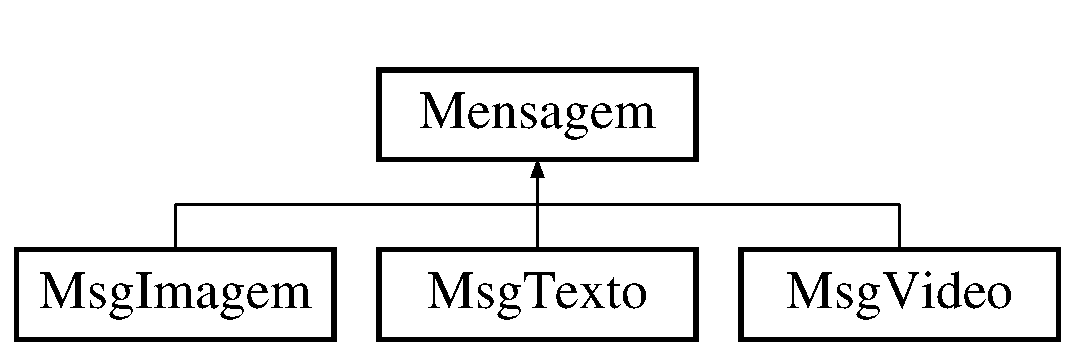
\includegraphics[height=2.000000cm]{class_mensagem}
\end{center}
\end{figure}
\subsection*{Public Member Functions}
\begin{DoxyCompactItemize}
\item 
\hyperlink{class_mensagem_a4152f41a1dbfd03eb058d6a9926f4426}{Mensagem} (\hyperlink{class_data}{Data} data, \hyperlink{class_horas}{Horas} hora)
\begin{DoxyCompactList}\small\item\em Construtor da classe \hyperlink{class_mensagem}{Mensagem};. \end{DoxyCompactList}\item 
\hypertarget{class_mensagem_a4490a1cfe88288fa1ff4b41327e769ed}{}virtual void \hyperlink{class_mensagem_a4490a1cfe88288fa1ff4b41327e769ed}{imprimir\+Msg} ()\label{class_mensagem_a4490a1cfe88288fa1ff4b41327e769ed}

\begin{DoxyCompactList}\small\item\em Funcao que imprime todos os membros privados da mensagem. \end{DoxyCompactList}\item 
string \hyperlink{class_mensagem_a5438dfe93aec2e6512042704e134d5db}{get\+Emissor} () const 
\begin{DoxyCompactList}\small\item\em Funcao que retorna o emissor. \end{DoxyCompactList}\item 
\hyperlink{class_data}{Data} \hyperlink{class_mensagem_a8d3b52e1c20fac96c4df60c79b5b7846}{get\+Data} () const 
\begin{DoxyCompactList}\small\item\em Funcao que retorna a data. \end{DoxyCompactList}\item 
\hyperlink{class_horas}{Horas} \hyperlink{class_mensagem_a7285a85c11aea596e25c6f87a68ad86f}{get\+Hora} () const 
\begin{DoxyCompactList}\small\item\em Funcao que retorna a hora. \end{DoxyCompactList}\item 
int \hyperlink{class_mensagem_a376309b58e69c41bf10acb7adad7bd3d}{get\+Numero} () const 
\begin{DoxyCompactList}\small\item\em Funcao que retorna o numero. \end{DoxyCompactList}\item 
void \hyperlink{class_mensagem_a74d42818d3796b28496f400e02328c92}{set\+Emissor} (string emissor)
\begin{DoxyCompactList}\small\item\em Funcao que altera o emissor. \end{DoxyCompactList}\item 
void \hyperlink{class_mensagem_a042a57d4dca817ed0450340b42111a9a}{set\+Numero} (int num)
\begin{DoxyCompactList}\small\item\em Funcao que altera o numero da mensagem. \end{DoxyCompactList}\end{DoxyCompactItemize}
\subsection*{Static Public Member Functions}
\begin{DoxyCompactItemize}
\item 
static int \hyperlink{class_mensagem_aedda3752e5473856e88644839a16fb10}{get\+I\+D} ()
\begin{DoxyCompactList}\small\item\em Funcao que retorna o id. \end{DoxyCompactList}\end{DoxyCompactItemize}


\subsection{Detailed Description}
Classe \hyperlink{class_mensagem}{Mensagem}. Cada \hyperlink{class_mensagem}{Mensagem} tem um id unico que representa o numero da mensgem. Cata \hyperlink{class_mensagem}{Mensagem} pode ainda ser de texto, video ou imagem. 

\subsection{Constructor \& Destructor Documentation}
\hypertarget{class_mensagem_a4152f41a1dbfd03eb058d6a9926f4426}{}\index{Mensagem@{Mensagem}!Mensagem@{Mensagem}}
\index{Mensagem@{Mensagem}!Mensagem@{Mensagem}}
\subsubsection[{Mensagem(\+Data data, Horas hora)}]{\setlength{\rightskip}{0pt plus 5cm}Mensagem\+::\+Mensagem (
\begin{DoxyParamCaption}
\item[{{\bf Data}}]{data, }
\item[{{\bf Horas}}]{hora}
\end{DoxyParamCaption}
)}\label{class_mensagem_a4152f41a1dbfd03eb058d6a9926f4426}


Construtor da classe \hyperlink{class_mensagem}{Mensagem};. 


\begin{DoxyParams}{Parameters}
{\em data} & \hyperlink{class_data}{Data} de criacao \\
\hline
{\em hora} & Hora de criacao \\
\hline
\end{DoxyParams}


\subsection{Member Function Documentation}
\hypertarget{class_mensagem_a8d3b52e1c20fac96c4df60c79b5b7846}{}\index{Mensagem@{Mensagem}!get\+Data@{get\+Data}}
\index{get\+Data@{get\+Data}!Mensagem@{Mensagem}}
\subsubsection[{get\+Data() const }]{\setlength{\rightskip}{0pt plus 5cm}{\bf Data} Mensagem\+::get\+Data (
\begin{DoxyParamCaption}
{}
\end{DoxyParamCaption}
) const}\label{class_mensagem_a8d3b52e1c20fac96c4df60c79b5b7846}


Funcao que retorna a data. 

\begin{DoxyReturn}{Returns}
data 
\end{DoxyReturn}
\hypertarget{class_mensagem_a5438dfe93aec2e6512042704e134d5db}{}\index{Mensagem@{Mensagem}!get\+Emissor@{get\+Emissor}}
\index{get\+Emissor@{get\+Emissor}!Mensagem@{Mensagem}}
\subsubsection[{get\+Emissor() const }]{\setlength{\rightskip}{0pt plus 5cm}string Mensagem\+::get\+Emissor (
\begin{DoxyParamCaption}
{}
\end{DoxyParamCaption}
) const}\label{class_mensagem_a5438dfe93aec2e6512042704e134d5db}


Funcao que retorna o emissor. 

\begin{DoxyReturn}{Returns}
emissor 
\end{DoxyReturn}
\hypertarget{class_mensagem_a7285a85c11aea596e25c6f87a68ad86f}{}\index{Mensagem@{Mensagem}!get\+Hora@{get\+Hora}}
\index{get\+Hora@{get\+Hora}!Mensagem@{Mensagem}}
\subsubsection[{get\+Hora() const }]{\setlength{\rightskip}{0pt plus 5cm}{\bf Horas} Mensagem\+::get\+Hora (
\begin{DoxyParamCaption}
{}
\end{DoxyParamCaption}
) const}\label{class_mensagem_a7285a85c11aea596e25c6f87a68ad86f}


Funcao que retorna a hora. 

\begin{DoxyReturn}{Returns}
hora 
\end{DoxyReturn}
\hypertarget{class_mensagem_aedda3752e5473856e88644839a16fb10}{}\index{Mensagem@{Mensagem}!get\+I\+D@{get\+I\+D}}
\index{get\+I\+D@{get\+I\+D}!Mensagem@{Mensagem}}
\subsubsection[{get\+I\+D()}]{\setlength{\rightskip}{0pt plus 5cm}static int Mensagem\+::get\+I\+D (
\begin{DoxyParamCaption}
{}
\end{DoxyParamCaption}
)\hspace{0.3cm}{\ttfamily [inline]}, {\ttfamily [static]}}\label{class_mensagem_aedda3752e5473856e88644839a16fb10}


Funcao que retorna o id. 

\begin{DoxyReturn}{Returns}
id 
\end{DoxyReturn}
\hypertarget{class_mensagem_a376309b58e69c41bf10acb7adad7bd3d}{}\index{Mensagem@{Mensagem}!get\+Numero@{get\+Numero}}
\index{get\+Numero@{get\+Numero}!Mensagem@{Mensagem}}
\subsubsection[{get\+Numero() const }]{\setlength{\rightskip}{0pt plus 5cm}int Mensagem\+::get\+Numero (
\begin{DoxyParamCaption}
{}
\end{DoxyParamCaption}
) const}\label{class_mensagem_a376309b58e69c41bf10acb7adad7bd3d}


Funcao que retorna o numero. 

\begin{DoxyReturn}{Returns}
numero 
\end{DoxyReturn}
\hypertarget{class_mensagem_a74d42818d3796b28496f400e02328c92}{}\index{Mensagem@{Mensagem}!set\+Emissor@{set\+Emissor}}
\index{set\+Emissor@{set\+Emissor}!Mensagem@{Mensagem}}
\subsubsection[{set\+Emissor(string emissor)}]{\setlength{\rightskip}{0pt plus 5cm}void Mensagem\+::set\+Emissor (
\begin{DoxyParamCaption}
\item[{string}]{emissor}
\end{DoxyParamCaption}
)}\label{class_mensagem_a74d42818d3796b28496f400e02328c92}


Funcao que altera o emissor. 


\begin{DoxyParams}{Parameters}
{\em emissor} & \\
\hline
\end{DoxyParams}
\hypertarget{class_mensagem_a042a57d4dca817ed0450340b42111a9a}{}\index{Mensagem@{Mensagem}!set\+Numero@{set\+Numero}}
\index{set\+Numero@{set\+Numero}!Mensagem@{Mensagem}}
\subsubsection[{set\+Numero(int num)}]{\setlength{\rightskip}{0pt plus 5cm}void Mensagem\+::set\+Numero (
\begin{DoxyParamCaption}
\item[{int}]{num}
\end{DoxyParamCaption}
)}\label{class_mensagem_a042a57d4dca817ed0450340b42111a9a}


Funcao que altera o numero da mensagem. 


\begin{DoxyParams}{Parameters}
{\em num} & Numero novo \\
\hline
\end{DoxyParams}


The documentation for this class was generated from the following files\+:\begin{DoxyCompactItemize}
\item 
Mensagem.\+h\item 
Mensagem.\+cpp\end{DoxyCompactItemize}

\hypertarget{class_msg_imagem}{}\section{Msg\+Imagem Class Reference}
\label{class_msg_imagem}\index{Msg\+Imagem@{Msg\+Imagem}}
Inheritance diagram for Msg\+Imagem\+:\begin{figure}[H]
\begin{center}
\leavevmode
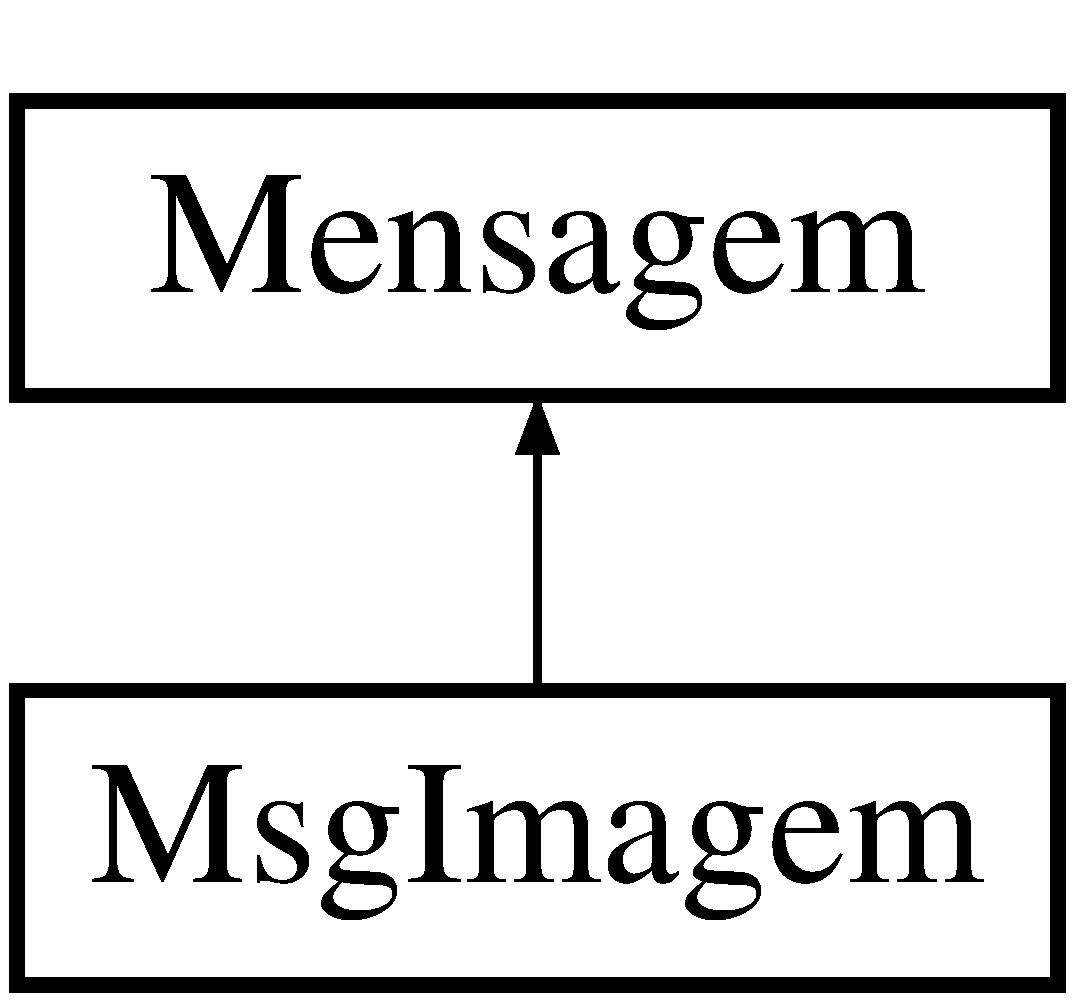
\includegraphics[height=2.000000cm]{class_msg_imagem}
\end{center}
\end{figure}
\subsection*{Public Member Functions}
\begin{DoxyCompactItemize}
\item 
\hypertarget{class_msg_imagem_af214317005643374b9886897ddc28e9c}{}{\bfseries Msg\+Imagem} (\hyperlink{class_data}{Data} d, \hyperlink{class_horas}{Horas} h)\label{class_msg_imagem_af214317005643374b9886897ddc28e9c}

\item 
\hypertarget{class_msg_imagem_a70e0cf4e47ecaee095501d211e010e27}{}void {\bfseries imprimir\+Msg} ()\label{class_msg_imagem_a70e0cf4e47ecaee095501d211e010e27}

\end{DoxyCompactItemize}
\subsection*{Additional Inherited Members}


The documentation for this class was generated from the following files\+:\begin{DoxyCompactItemize}
\item 
Mensagem.\+h\item 
Mensagem.\+cpp\end{DoxyCompactItemize}

\hypertarget{class_msg_texto}{}\section{Msg\+Texto Class Reference}
\label{class_msg_texto}\index{Msg\+Texto@{Msg\+Texto}}


Classe \hyperlink{class_msg_texto}{Msg\+Texto}. E uma classe derivada da classe \hyperlink{class_mensagem}{Mensagem} que representa o tipo de mensagem.  




{\ttfamily \#include $<$Mensagem.\+h$>$}

Inheritance diagram for Msg\+Texto\+:\begin{figure}[H]
\begin{center}
\leavevmode
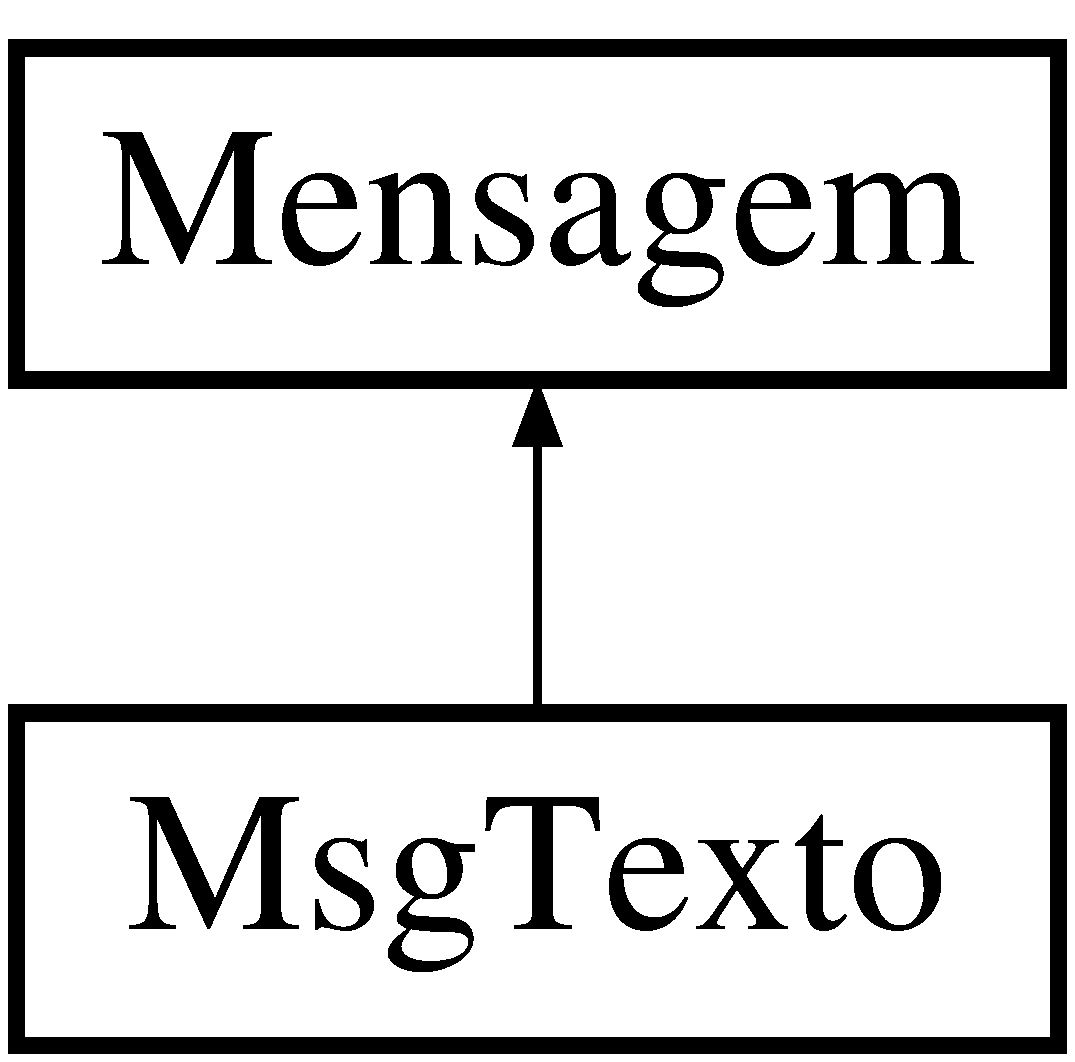
\includegraphics[height=2.000000cm]{class_msg_texto}
\end{center}
\end{figure}
\subsection*{Public Member Functions}
\begin{DoxyCompactItemize}
\item 
\hyperlink{class_msg_texto_a8ad133274a0f20954695cd2b2c619595}{Msg\+Texto} (string conteudo, \hyperlink{class_data}{Data} d, \hyperlink{class_horas}{Horas} h)
\begin{DoxyCompactList}\small\item\em Construtor de \hyperlink{class_msg_texto}{Msg\+Texto}. \end{DoxyCompactList}\item 
string \hyperlink{class_msg_texto_a9743e624bf980d9b4ed0db65a947f203}{get\+Conteudo} () const 
\begin{DoxyCompactList}\small\item\em Funcao que retorna o conteudo. \end{DoxyCompactList}\item 
\hypertarget{class_msg_texto_ac621ebd05f2c55fcfe9746ff402ab26b}{}void \hyperlink{class_msg_texto_ac621ebd05f2c55fcfe9746ff402ab26b}{imprimir\+Msg} ()\label{class_msg_texto_ac621ebd05f2c55fcfe9746ff402ab26b}

\begin{DoxyCompactList}\small\item\em Funcao que imprime no ecra a mensagem. \end{DoxyCompactList}\item 
string \hyperlink{class_msg_texto_acd54b047498f468c1f57a694c1bea591}{tipo} () const 
\begin{DoxyCompactList}\small\item\em Funcao que retorna o tipo de mensagem. \end{DoxyCompactList}\end{DoxyCompactItemize}
\subsection*{Additional Inherited Members}


\subsection{Detailed Description}
Classe \hyperlink{class_msg_texto}{Msg\+Texto}. E uma classe derivada da classe \hyperlink{class_mensagem}{Mensagem} que representa o tipo de mensagem. 

\subsection{Constructor \& Destructor Documentation}
\hypertarget{class_msg_texto_a8ad133274a0f20954695cd2b2c619595}{}\index{Msg\+Texto@{Msg\+Texto}!Msg\+Texto@{Msg\+Texto}}
\index{Msg\+Texto@{Msg\+Texto}!Msg\+Texto@{Msg\+Texto}}
\subsubsection[{Msg\+Texto(string conteudo, Data d, Horas h)}]{\setlength{\rightskip}{0pt plus 5cm}Msg\+Texto\+::\+Msg\+Texto (
\begin{DoxyParamCaption}
\item[{string}]{conteudo, }
\item[{{\bf Data}}]{d, }
\item[{{\bf Horas}}]{h}
\end{DoxyParamCaption}
)}\label{class_msg_texto_a8ad133274a0f20954695cd2b2c619595}


Construtor de \hyperlink{class_msg_texto}{Msg\+Texto}. 


\begin{DoxyParams}{Parameters}
{\em conteudo} & \\
\hline
{\em d} & data \\
\hline
{\em h} & hora \\
\hline
\end{DoxyParams}


\subsection{Member Function Documentation}
\hypertarget{class_msg_texto_a9743e624bf980d9b4ed0db65a947f203}{}\index{Msg\+Texto@{Msg\+Texto}!get\+Conteudo@{get\+Conteudo}}
\index{get\+Conteudo@{get\+Conteudo}!Msg\+Texto@{Msg\+Texto}}
\subsubsection[{get\+Conteudo() const }]{\setlength{\rightskip}{0pt plus 5cm}string Msg\+Texto\+::get\+Conteudo (
\begin{DoxyParamCaption}
{}
\end{DoxyParamCaption}
) const\hspace{0.3cm}{\ttfamily [virtual]}}\label{class_msg_texto_a9743e624bf980d9b4ed0db65a947f203}


Funcao que retorna o conteudo. 

\begin{DoxyReturn}{Returns}
conteudo 
\end{DoxyReturn}


Reimplemented from \hyperlink{class_mensagem_ab4bbb32ae268565c8f87c370f9793db6}{Mensagem}.

\hypertarget{class_msg_texto_acd54b047498f468c1f57a694c1bea591}{}\index{Msg\+Texto@{Msg\+Texto}!tipo@{tipo}}
\index{tipo@{tipo}!Msg\+Texto@{Msg\+Texto}}
\subsubsection[{tipo() const }]{\setlength{\rightskip}{0pt plus 5cm}string Msg\+Texto\+::tipo (
\begin{DoxyParamCaption}
{}
\end{DoxyParamCaption}
) const\hspace{0.3cm}{\ttfamily [virtual]}}\label{class_msg_texto_acd54b047498f468c1f57a694c1bea591}


Funcao que retorna o tipo de mensagem. 

\begin{DoxyReturn}{Returns}
string com t 
\end{DoxyReturn}


Reimplemented from \hyperlink{class_mensagem_a3d814fb7b7540c4df98f522208e0c1ac}{Mensagem}.



The documentation for this class was generated from the following files\+:\begin{DoxyCompactItemize}
\item 
Mensagem.\+h\item 
Mensagem.\+cpp\end{DoxyCompactItemize}

\hypertarget{class_msg_video}{}\section{Msg\+Video Class Reference}
\label{class_msg_video}\index{Msg\+Video@{Msg\+Video}}
Inheritance diagram for Msg\+Video\+:\begin{figure}[H]
\begin{center}
\leavevmode
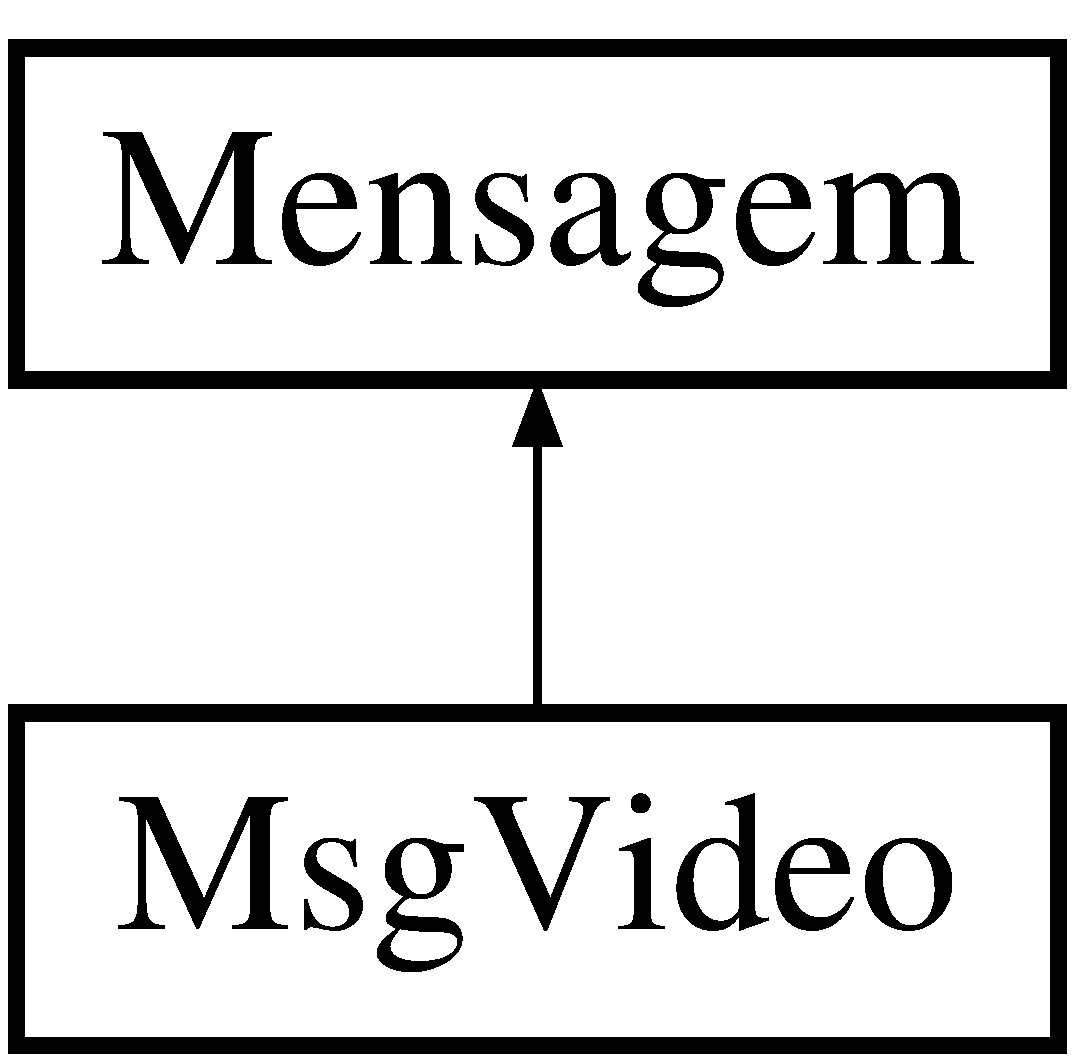
\includegraphics[height=2.000000cm]{class_msg_video}
\end{center}
\end{figure}
\subsection*{Public Member Functions}
\begin{DoxyCompactItemize}
\item 
\hypertarget{class_msg_video_aef9a682492022a03ff4ea1ab62e1e1f9}{}{\bfseries Msg\+Video} (\hyperlink{class_data}{Data} d, \hyperlink{class_horas}{Horas} h)\label{class_msg_video_aef9a682492022a03ff4ea1ab62e1e1f9}

\item 
\hypertarget{class_msg_video_a9073f476d181d88e03c6cbf4c283533d}{}void {\bfseries imprimir\+Msg} ()\label{class_msg_video_a9073f476d181d88e03c6cbf4c283533d}

\end{DoxyCompactItemize}
\subsection*{Additional Inherited Members}


The documentation for this class was generated from the following files\+:\begin{DoxyCompactItemize}
\item 
Mensagem.\+h\item 
Mensagem.\+cpp\end{DoxyCompactItemize}

\hypertarget{class_nao_moderador}{}\section{Nao\+Moderador Class Reference}
\label{class_nao_moderador}\index{Nao\+Moderador@{Nao\+Moderador}}


Classe que representa uma excecao da classe grupo. Esta excecao e lancada no caso de o utilizador que esta a pedir permissoes nao ser o utilizador moderador do grupo.  




{\ttfamily \#include $<$Excecoes.\+h$>$}

\subsection*{Public Member Functions}
\begin{DoxyCompactItemize}
\item 
\hyperlink{class_nao_moderador_aa57843875543c5246fc733f87b6ef3dd}{Nao\+Moderador} (string mod)
\begin{DoxyCompactList}\small\item\em Construtor. Inicializa o membro mod com o utilizador recebido. \end{DoxyCompactList}\item 
string \hyperlink{class_nao_moderador_aff0ecf62b3446554d93d4032276a6f29}{get\+Nome} () const 
\begin{DoxyCompactList}\small\item\em Funcao que retorna o utilizador. \end{DoxyCompactList}\end{DoxyCompactItemize}


\subsection{Detailed Description}
Classe que representa uma excecao da classe grupo. Esta excecao e lancada no caso de o utilizador que esta a pedir permissoes nao ser o utilizador moderador do grupo. 

\subsection{Constructor \& Destructor Documentation}
\hypertarget{class_nao_moderador_aa57843875543c5246fc733f87b6ef3dd}{}\index{Nao\+Moderador@{Nao\+Moderador}!Nao\+Moderador@{Nao\+Moderador}}
\index{Nao\+Moderador@{Nao\+Moderador}!Nao\+Moderador@{Nao\+Moderador}}
\subsubsection[{Nao\+Moderador(string mod)}]{\setlength{\rightskip}{0pt plus 5cm}Nao\+Moderador\+::\+Nao\+Moderador (
\begin{DoxyParamCaption}
\item[{string}]{mod}
\end{DoxyParamCaption}
)\hspace{0.3cm}{\ttfamily [inline]}}\label{class_nao_moderador_aa57843875543c5246fc733f87b6ef3dd}


Construtor. Inicializa o membro mod com o utilizador recebido. 


\begin{DoxyParams}{Parameters}
{\em mod} & \hyperlink{class_utilizador}{Utilizador} recebido. \\
\hline
\end{DoxyParams}


\subsection{Member Function Documentation}
\hypertarget{class_nao_moderador_aff0ecf62b3446554d93d4032276a6f29}{}\index{Nao\+Moderador@{Nao\+Moderador}!get\+Nome@{get\+Nome}}
\index{get\+Nome@{get\+Nome}!Nao\+Moderador@{Nao\+Moderador}}
\subsubsection[{get\+Nome() const }]{\setlength{\rightskip}{0pt plus 5cm}string Nao\+Moderador\+::get\+Nome (
\begin{DoxyParamCaption}
{}
\end{DoxyParamCaption}
) const\hspace{0.3cm}{\ttfamily [inline]}}\label{class_nao_moderador_aff0ecf62b3446554d93d4032276a6f29}


Funcao que retorna o utilizador. 

\begin{DoxyReturn}{Returns}
mod 
\end{DoxyReturn}


The documentation for this class was generated from the following file\+:\begin{DoxyCompactItemize}
\item 
Excecoes.\+h\end{DoxyCompactItemize}

\hypertarget{class_nao_participante}{}\section{Nao\+Participante Class Reference}
\label{class_nao_participante}\index{Nao\+Participante@{Nao\+Participante}}


Classe que representa uma excecao da classe conversa. Esta excecao e lancada quando um utilizador que nao participa na conversa tenta enviar mensagens.  




{\ttfamily \#include $<$Excecoes.\+h$>$}

\subsection*{Public Member Functions}
\begin{DoxyCompactItemize}
\item 
\hyperlink{class_nao_participante_af0a256b2f1b44f856076b083966793f6}{Nao\+Participante} (string p)
\begin{DoxyCompactList}\small\item\em Construtor. Inicializa o membro p com o login do utilizador que nao e participante. \end{DoxyCompactList}\item 
string \hyperlink{class_nao_participante_a6199680fa5f2abfb8abb583d11fc3fd9}{getlogin} () const 
\begin{DoxyCompactList}\small\item\em Funcao que retorna o login do nao participante. \end{DoxyCompactList}\end{DoxyCompactItemize}


\subsection{Detailed Description}
Classe que representa uma excecao da classe conversa. Esta excecao e lancada quando um utilizador que nao participa na conversa tenta enviar mensagens. 

\subsection{Constructor \& Destructor Documentation}
\hypertarget{class_nao_participante_af0a256b2f1b44f856076b083966793f6}{}\index{Nao\+Participante@{Nao\+Participante}!Nao\+Participante@{Nao\+Participante}}
\index{Nao\+Participante@{Nao\+Participante}!Nao\+Participante@{Nao\+Participante}}
\subsubsection[{Nao\+Participante(string p)}]{\setlength{\rightskip}{0pt plus 5cm}Nao\+Participante\+::\+Nao\+Participante (
\begin{DoxyParamCaption}
\item[{string}]{p}
\end{DoxyParamCaption}
)\hspace{0.3cm}{\ttfamily [inline]}}\label{class_nao_participante_af0a256b2f1b44f856076b083966793f6}


Construtor. Inicializa o membro p com o login do utilizador que nao e participante. 


\begin{DoxyParams}{Parameters}
{\em p} & Login do participante. \\
\hline
\end{DoxyParams}


\subsection{Member Function Documentation}
\hypertarget{class_nao_participante_a6199680fa5f2abfb8abb583d11fc3fd9}{}\index{Nao\+Participante@{Nao\+Participante}!getlogin@{getlogin}}
\index{getlogin@{getlogin}!Nao\+Participante@{Nao\+Participante}}
\subsubsection[{getlogin() const }]{\setlength{\rightskip}{0pt plus 5cm}string Nao\+Participante\+::getlogin (
\begin{DoxyParamCaption}
{}
\end{DoxyParamCaption}
) const\hspace{0.3cm}{\ttfamily [inline]}}\label{class_nao_participante_a6199680fa5f2abfb8abb583d11fc3fd9}


Funcao que retorna o login do nao participante. 

\begin{DoxyReturn}{Returns}
p Login do utilizador nao participante 
\end{DoxyReturn}


The documentation for this class was generated from the following file\+:\begin{DoxyCompactItemize}
\item 
Excecoes.\+h\end{DoxyCompactItemize}

\hypertarget{class_opccao_invalida}{}\section{Opccao\+Invalida$<$ N $>$ Class Template Reference}
\label{class_opccao_invalida}\index{Opccao\+Invalida$<$ N $>$@{Opccao\+Invalida$<$ N $>$}}


Classe que representa uma excecao da classe Main. Esta excecao e lancada quando a opcao colocada nao esta entre os limites estabelecidos. E uma classe template pois pode receber mais que um tipo de dados.  




{\ttfamily \#include $<$Excecoes.\+h$>$}

\subsection*{Public Member Functions}
\begin{DoxyCompactItemize}
\item 
\hyperlink{class_opccao_invalida_a19b191db4d1cc8c074c24a940571dd4b}{Opccao\+Invalida} (N op, N min, N max)
\begin{DoxyCompactList}\small\item\em Construtor. Inicializa os membros op, min e max com, repetivamente, a opcao escolhida, a opcao minima e a opcao maxima. \end{DoxyCompactList}\item 
\hypertarget{class_opccao_invalida_abac2e9c809f6b1dc5e0179e28604f528}{}N {\bfseries get\+Min} () const \label{class_opccao_invalida_abac2e9c809f6b1dc5e0179e28604f528}

\item 
\hypertarget{class_opccao_invalida_a98bb7934220a9b27b9da823207b72db3}{}N {\bfseries get\+Max} () const \label{class_opccao_invalida_a98bb7934220a9b27b9da823207b72db3}

\item 
N \hyperlink{class_opccao_invalida_ac9afa1ee68970cddd39a9873fd2c357f}{get\+Op} () const 
\begin{DoxyCompactList}\small\item\em Funcao que retorna a opcao escolhida. \end{DoxyCompactList}\end{DoxyCompactItemize}


\subsection{Detailed Description}
\subsubsection*{template$<$class N$>$class Opccao\+Invalida$<$ N $>$}

Classe que representa uma excecao da classe Main. Esta excecao e lancada quando a opcao colocada nao esta entre os limites estabelecidos. E uma classe template pois pode receber mais que um tipo de dados. 

\subsection{Constructor \& Destructor Documentation}
\hypertarget{class_opccao_invalida_a19b191db4d1cc8c074c24a940571dd4b}{}\index{Opccao\+Invalida@{Opccao\+Invalida}!Opccao\+Invalida@{Opccao\+Invalida}}
\index{Opccao\+Invalida@{Opccao\+Invalida}!Opccao\+Invalida@{Opccao\+Invalida}}
\subsubsection[{Opccao\+Invalida(\+N op, N min, N max)}]{\setlength{\rightskip}{0pt plus 5cm}template$<$class N $>$ {\bf Opccao\+Invalida}$<$ N $>$\+::{\bf Opccao\+Invalida} (
\begin{DoxyParamCaption}
\item[{N}]{op, }
\item[{N}]{min, }
\item[{N}]{max}
\end{DoxyParamCaption}
)\hspace{0.3cm}{\ttfamily [inline]}}\label{class_opccao_invalida_a19b191db4d1cc8c074c24a940571dd4b}


Construtor. Inicializa os membros op, min e max com, repetivamente, a opcao escolhida, a opcao minima e a opcao maxima. 


\begin{DoxyParams}{Parameters}
{\em op} & Opcao escolhida. \\
\hline
{\em min} & Opcao minima. \\
\hline
{\em max} & Opcao maxima. \\
\hline
\end{DoxyParams}


\subsection{Member Function Documentation}
\hypertarget{class_opccao_invalida_ac9afa1ee68970cddd39a9873fd2c357f}{}\index{Opccao\+Invalida@{Opccao\+Invalida}!get\+Op@{get\+Op}}
\index{get\+Op@{get\+Op}!Opccao\+Invalida@{Opccao\+Invalida}}
\subsubsection[{get\+Op() const }]{\setlength{\rightskip}{0pt plus 5cm}template$<$class N $>$ N {\bf Opccao\+Invalida}$<$ N $>$\+::get\+Op (
\begin{DoxyParamCaption}
{}
\end{DoxyParamCaption}
) const\hspace{0.3cm}{\ttfamily [inline]}}\label{class_opccao_invalida_ac9afa1ee68970cddd39a9873fd2c357f}


Funcao que retorna a opcao escolhida. 

\begin{DoxyReturn}{Returns}
Opcao escolhida. 
\end{DoxyReturn}


The documentation for this class was generated from the following file\+:\begin{DoxyCompactItemize}
\item 
Excecoes.\+h\end{DoxyCompactItemize}

\hypertarget{class_pedido_inexistente}{}\section{Pedido\+Inexistente Class Reference}
\label{class_pedido_inexistente}\index{Pedido\+Inexistente@{Pedido\+Inexistente}}


Classe que representa uma excecao da classe grupo. Esta excecao e lancada quando nao existe no vetor de pedidos de adesao de um grupo o login recebido.  




{\ttfamily \#include $<$Excecoes.\+h$>$}

\subsection*{Public Member Functions}
\begin{DoxyCompactItemize}
\item 
\hyperlink{class_pedido_inexistente_ae30b81fc0eff41039f0efd87b055daca}{Pedido\+Inexistente} (string l)
\begin{DoxyCompactList}\small\item\em Construtor. Inicializa o membro login com o login do utilizador que criou a excecao. \end{DoxyCompactList}\item 
string \hyperlink{class_pedido_inexistente_a4922d9813deb3df3880405abef24cc74}{get\+Login} () const 
\begin{DoxyCompactList}\small\item\em Funcao que retorna o login do utilizador. \end{DoxyCompactList}\end{DoxyCompactItemize}


\subsection{Detailed Description}
Classe que representa uma excecao da classe grupo. Esta excecao e lancada quando nao existe no vetor de pedidos de adesao de um grupo o login recebido. 

\subsection{Constructor \& Destructor Documentation}
\hypertarget{class_pedido_inexistente_ae30b81fc0eff41039f0efd87b055daca}{}\index{Pedido\+Inexistente@{Pedido\+Inexistente}!Pedido\+Inexistente@{Pedido\+Inexistente}}
\index{Pedido\+Inexistente@{Pedido\+Inexistente}!Pedido\+Inexistente@{Pedido\+Inexistente}}
\subsubsection[{Pedido\+Inexistente(string l)}]{\setlength{\rightskip}{0pt plus 5cm}Pedido\+Inexistente\+::\+Pedido\+Inexistente (
\begin{DoxyParamCaption}
\item[{string}]{l}
\end{DoxyParamCaption}
)\hspace{0.3cm}{\ttfamily [inline]}}\label{class_pedido_inexistente_ae30b81fc0eff41039f0efd87b055daca}


Construtor. Inicializa o membro login com o login do utilizador que criou a excecao. 


\begin{DoxyParams}{Parameters}
{\em l} & Login recebido. \\
\hline
\end{DoxyParams}


\subsection{Member Function Documentation}
\hypertarget{class_pedido_inexistente_a4922d9813deb3df3880405abef24cc74}{}\index{Pedido\+Inexistente@{Pedido\+Inexistente}!get\+Login@{get\+Login}}
\index{get\+Login@{get\+Login}!Pedido\+Inexistente@{Pedido\+Inexistente}}
\subsubsection[{get\+Login() const }]{\setlength{\rightskip}{0pt plus 5cm}string Pedido\+Inexistente\+::get\+Login (
\begin{DoxyParamCaption}
{}
\end{DoxyParamCaption}
) const\hspace{0.3cm}{\ttfamily [inline]}}\label{class_pedido_inexistente_a4922d9813deb3df3880405abef24cc74}


Funcao que retorna o login do utilizador. 

\begin{DoxyReturn}{Returns}
login 
\end{DoxyReturn}


The documentation for this class was generated from the following file\+:\begin{DoxyCompactItemize}
\item 
Excecoes.\+h\end{DoxyCompactItemize}

\hypertarget{class_utilizador}{}\section{Utilizador Class Reference}
\label{class_utilizador}\index{Utilizador@{Utilizador}}


Classe \hyperlink{class_utilizador}{Utilizador}. Cada \hyperlink{class_utilizador}{Utilizador} tem como unico o seu login e tem que ter como obrigatorio maior de 18 anos. A Classe \hyperlink{class_utilizador}{Utilizador} permite ter conversas e grupos com aqueles que apenas fazem parte do seu grupo de amigos. Esta Classe permite a gestao e a criacao de novos objectos \hyperlink{class_grupo}{Grupo}, \hyperlink{class_conversa}{Conversa} e Mensagens.  




{\ttfamily \#include $<$Utilizador.\+h$>$}

\subsection*{Public Member Functions}
\begin{DoxyCompactItemize}
\item 
\hypertarget{class_utilizador_a264cb21da71b44fc2d5cfb21e58fa24a}{}\hyperlink{class_utilizador_a264cb21da71b44fc2d5cfb21e58fa24a}{Utilizador} ()\label{class_utilizador_a264cb21da71b44fc2d5cfb21e58fa24a}

\begin{DoxyCompactList}\small\item\em Construtor \hyperlink{class_utilizador}{Utilizador};. \end{DoxyCompactList}\item 
\hypertarget{class_utilizador_aa0c2432b0a0f7b64ca5e7232ceec2869}{}\hyperlink{class_utilizador_aa0c2432b0a0f7b64ca5e7232ceec2869}{$\sim$\+Utilizador} ()\label{class_utilizador_aa0c2432b0a0f7b64ca5e7232ceec2869}

\begin{DoxyCompactList}\small\item\em Destrutor \hyperlink{class_utilizador}{Utilizador};. \end{DoxyCompactList}\item 
\hyperlink{class_utilizador_a470435e7e91ef2aa93eaf97b0615499b}{Utilizador} (bool visibilidade, string login, string nome, string email, \hyperlink{class_data}{Data} data\+Adesao, int telemovel, int idade)
\begin{DoxyCompactList}\small\item\em Construtor classe \hyperlink{class_utilizador}{Utilizador}. \end{DoxyCompactList}\item 
string \hyperlink{class_utilizador_aa5af9c1385b0a93116dd8a80264b887a}{get\+Nome} () const 
\begin{DoxyCompactList}\small\item\em Funcao que retorna o nome do \hyperlink{class_utilizador}{Utilizador}. \end{DoxyCompactList}\item 
string \hyperlink{class_utilizador_a9fc99ac7634ff085ca0f3afd4d502cc7}{get\+Email} () const 
\begin{DoxyCompactList}\small\item\em Funcao que retorna o email do \hyperlink{class_utilizador}{Utilizador}. \end{DoxyCompactList}\item 
string \hyperlink{class_utilizador_ad6c565c391bd19de3462e50a4e05c9a6}{get\+Login} () const 
\begin{DoxyCompactList}\small\item\em Funcao que retorna o login do \hyperlink{class_utilizador}{Utilizador}. \end{DoxyCompactList}\item 
int \hyperlink{class_utilizador_a60b66b8e80767719861a2d712f1bcbe4}{get\+Telemovel} () const 
\begin{DoxyCompactList}\small\item\em Funcao que retorna o telemovel do \hyperlink{class_utilizador}{Utilizador}. \end{DoxyCompactList}\item 
int \hyperlink{class_utilizador_a9abaeb6fbff49683f57164a57e6f0c90}{get\+Idade} () const 
\begin{DoxyCompactList}\small\item\em Funcao que retorna a idade do \hyperlink{class_utilizador}{Utilizador}. \end{DoxyCompactList}\item 
bool \hyperlink{class_utilizador_a99cdee165a8446fb67f3e0cab0831e80}{get\+Visibilidade} () const 
\begin{DoxyCompactList}\small\item\em Funcao que retorna a visibilidade do \hyperlink{class_utilizador}{Utilizador}. \end{DoxyCompactList}\item 
\hyperlink{class_data}{Data} \hyperlink{class_utilizador_af6c41442d2029ccb1a135092a5c27007}{get\+Data\+Adesao} () const 
\begin{DoxyCompactList}\small\item\em Funcao que retorna a data de adesao do \hyperlink{class_utilizador}{Utilizador}. \end{DoxyCompactList}\item 
vector$<$ \hyperlink{class_utilizador}{Utilizador} $\ast$ $>$ \hyperlink{class_utilizador_ad76009d2278707a5c9a1e8088633cfd2}{get\+Amigos} () const 
\begin{DoxyCompactList}\small\item\em Funcao que retorna um vector de Utilizadores que sao os amigos do \hyperlink{class_utilizador}{Utilizador}. \end{DoxyCompactList}\item 
\hyperlink{class_utilizador}{Utilizador} $\ast$ \hyperlink{class_utilizador_a13a11370779713c7de00ea62f5c3799b}{get\+Amigo} (string login) const 
\begin{DoxyCompactList}\small\item\em Funcao que retorna um apontador para um \hyperlink{class_utilizador}{Utilizador} dos amigos com um determinado login. \end{DoxyCompactList}\item 
\hyperlink{class_grupo}{Grupo} $\ast$ \hyperlink{class_utilizador_a0b6cd97f274e49649b0c2c7ba0497261}{get\+Grupo} (int i) const 
\begin{DoxyCompactList}\small\item\em Funcao que retorna um apontador para um \hyperlink{class_grupo}{Grupo} dos grupos de conversa de indice i. \end{DoxyCompactList}\item 
vector$<$ \hyperlink{class_grupo}{Grupo} $\ast$ $>$ \hyperlink{class_utilizador_ad3f06aaa4199be8c1742e7126633ec26}{get\+Grupos} () const 
\begin{DoxyCompactList}\small\item\em Funcao que retorna os grupos do utilizador. \end{DoxyCompactList}\item 
\hyperlink{class_conversa}{Conversa} $\ast$ \hyperlink{class_utilizador_a07745e2c5f5d9236aea0c7357f1325b7}{get\+Conversa} (int i) const 
\begin{DoxyCompactList}\small\item\em Funcao que retorna a conversa na posicao i. \end{DoxyCompactList}\item 
string \hyperlink{class_utilizador_a5d4275b4d23d955ef295773d3d9eb3b5}{get\+Destinatario\+Conversa} (\hyperlink{class_conversa}{Conversa} $\ast$c) const 
\begin{DoxyCompactList}\small\item\em Funcao que retorna o nome destinatario da \hyperlink{class_conversa}{Conversa}. \end{DoxyCompactList}\item 
vector$<$ \hyperlink{class_grupo}{Grupo} $\ast$ $>$ \hyperlink{class_utilizador_ac5e58137167b1cf097d10f862f036998}{get\+Grupos\+Amigos} () const 
\begin{DoxyCompactList}\small\item\em Funcao que retorna um vector com os grupos do meu circulo de amigos. Esta funcao retira os grupos repetidos e os grupos que ja incluem o utilizador atual. \end{DoxyCompactList}\item 
void \hyperlink{class_utilizador_a11032f76b9d07c21e9111155519407c5}{set\+Login} (string l)
\begin{DoxyCompactList}\small\item\em Funcao que altera o login de um utilizador. \end{DoxyCompactList}\item 
void \hyperlink{class_utilizador_a27aeea3bb85f457a2d42ff6f0a1240dd}{set\+Nome} (string n)
\begin{DoxyCompactList}\small\item\em Funcao que altera o nome de um utilizador. \end{DoxyCompactList}\item 
void \hyperlink{class_utilizador_aa5ad3c6ed417e2b3aebc96bfa5432dfb}{set\+Email} (string e)
\begin{DoxyCompactList}\small\item\em Funcao que altera o email de um utilizador. \end{DoxyCompactList}\item 
void \hyperlink{class_utilizador_aacc48e9ec11446c11029c3d062533034}{set\+Idade} (int i)
\begin{DoxyCompactList}\small\item\em Funcao que altera a idade do \hyperlink{class_utilizador}{Utilizador} lanca a excep��o \hyperlink{class_idade_insuficiente}{Idade\+Insuficiente} se for $<$ 18. \end{DoxyCompactList}\item 
void \hyperlink{class_utilizador_a2228288656c31e63710c31bf0d8eb58f}{set\+Visibilidade} (bool v)
\begin{DoxyCompactList}\small\item\em Funcao que altera a visibilidade de um utilizador. \end{DoxyCompactList}\item 
void \hyperlink{class_utilizador_a74e3737924910c4306bac26cacb5f8e1}{set\+Telemovel} (int t)
\begin{DoxyCompactList}\small\item\em Funcao que altera o telemovel de um utilizador. \end{DoxyCompactList}\item 
void \hyperlink{class_utilizador_a8cd2a3b9c962eeef6ffa497ce6e39a3c}{set\+Data} (int d, int m, int a)
\begin{DoxyCompactList}\small\item\em Funcao que altera a data de adesao de um utilizador. \end{DoxyCompactList}\item 
void \hyperlink{class_utilizador_a4b31c37715158bd7f672b8d2a546883f}{add\+Amigos\+Aux} (\hyperlink{class_utilizador}{Utilizador} $\ast$u)
\begin{DoxyCompactList}\small\item\em Funcao que adiciona um utilizador aos amigos do utilizador. \end{DoxyCompactList}\item 
void \hyperlink{class_utilizador_a896ea43c9f3c7224b2985b012e14b70d}{add\+Amigo} (\hyperlink{class_utilizador}{Utilizador} \&u)
\begin{DoxyCompactList}\small\item\em Funcao que adiciona um utilizador como amigos chama a funcao add\+Amigos\+Aux para adicionar o utilizador u aos meus amigos e para eu ser adicionado aos amigos de u. \end{DoxyCompactList}\item 
bool \hyperlink{class_utilizador_ac67ae90cd1dd3f13884ae905536741ea}{add\+Grupo} (\hyperlink{class_grupo}{Grupo} $\ast$g)
\begin{DoxyCompactList}\small\item\em Funcao que adiciona um grupo aos grupos do utilizador se o grupo nao pertencer aos meus grupos. \end{DoxyCompactList}\item 
void \hyperlink{class_utilizador_ad17ea854a0b048c52cc0bda0682a6533}{add\+Conversa} (\hyperlink{class_conversa}{Conversa} $\ast$c)
\begin{DoxyCompactList}\small\item\em Funcao que adiciona uma conversa as conversas do utilizador se a conversa j� n�o existir. \end{DoxyCompactList}\item 
bool \hyperlink{class_utilizador_a355f9a633b971d28a926cfcb3a20f8a7}{adiciona\+Membro} (\hyperlink{class_utilizador}{Utilizador} $\ast$u, \hyperlink{class_grupo}{Grupo} $\ast$g, \hyperlink{class_data}{Data} d)
\begin{DoxyCompactList}\small\item\em Funcao que adiciona um utilizador u a um grupo g, por iniciativa propria do moderador (sem pedido de adesao) Esta funcao chama a funcao adicionar\+Membro da classe grupo e coloca no vetor de grupos de u o novo grupo a que foi adicionado. \end{DoxyCompactList}\item 
void \hyperlink{class_utilizador_ac779bbfd15bd307b86cc7c06793509a2}{remover\+Amigo\+Aux} (\hyperlink{class_utilizador}{Utilizador} $\ast$u)
\begin{DoxyCompactList}\small\item\em Funcao que retira o utilizador u dos amigos do utilizador. \end{DoxyCompactList}\item 
void \hyperlink{class_utilizador_aeea440a088526eea36ebcc27d6472e4f}{remover\+Amigo} (\hyperlink{class_utilizador}{Utilizador} \&u)
\begin{DoxyCompactList}\small\item\em Funcao que remove u dos meus amigos e eu dos amigos de u usando a fun$\sim$cao remover\+Amigo\+Aux. \end{DoxyCompactList}\item 
bool \hyperlink{class_utilizador_a05e62bd42a3e3a324cea8d9c998c2391}{remover\+Membro} (\hyperlink{class_utilizador}{Utilizador} $\ast$u, \hyperlink{class_grupo}{Grupo} $\ast$g, \hyperlink{class_data}{Data} dia\+Atual)
\begin{DoxyCompactList}\small\item\em Funcao que remove um utilizador u de um grupo g. \end{DoxyCompactList}\item 
void \hyperlink{class_utilizador_a2f5cc4525c249995615ec7693230ee0d}{remover\+Conversa} (\hyperlink{class_conversa}{Conversa} $\ast$c)
\begin{DoxyCompactList}\small\item\em Funcao que remove a conversa c das conversas do utilizador. \end{DoxyCompactList}\item 
\hypertarget{class_utilizador_a1d4b8650dfe1d7a86f10192153e132d5}{}void \hyperlink{class_utilizador_a1d4b8650dfe1d7a86f10192153e132d5}{imprimir\+Definicoes} () const \label{class_utilizador_a1d4b8650dfe1d7a86f10192153e132d5}

\begin{DoxyCompactList}\small\item\em Funcao que imprime no ecra as definicoes do utilizador. \end{DoxyCompactList}\item 
\hypertarget{class_utilizador_abf2814a0783cdc5ef39326981474767b}{}void \hyperlink{class_utilizador_abf2814a0783cdc5ef39326981474767b}{imprimir\+Utilizador} () const \label{class_utilizador_abf2814a0783cdc5ef39326981474767b}

\begin{DoxyCompactList}\small\item\em Funcao que imprime no ecra o perfil do utilizador com as informa��es do mesmo dependendo da visibilidade. \end{DoxyCompactList}\item 
\hypertarget{class_utilizador_a433c888d3d5d669cda5fcb8d22832b37}{}void \hyperlink{class_utilizador_a433c888d3d5d669cda5fcb8d22832b37}{imprimir\+Amigos} () const \label{class_utilizador_a433c888d3d5d669cda5fcb8d22832b37}

\begin{DoxyCompactList}\small\item\em Funcao que imprime no ecra os amigos do utilizador. \end{DoxyCompactList}\item 
\hypertarget{class_utilizador_ad4bf7b549a337d684e43189db2d0d57c}{}void \hyperlink{class_utilizador_ad4bf7b549a337d684e43189db2d0d57c}{imprimir\+Grupos} () const \label{class_utilizador_ad4bf7b549a337d684e43189db2d0d57c}

\begin{DoxyCompactList}\small\item\em Funcao que imprime no ecra os grupos do utilizador. \end{DoxyCompactList}\item 
\hypertarget{class_utilizador_a14ea24f6a46b47206709bbb1c99247b2}{}void \hyperlink{class_utilizador_a14ea24f6a46b47206709bbb1c99247b2}{imprimir\+Conversas} () const \label{class_utilizador_a14ea24f6a46b47206709bbb1c99247b2}

\begin{DoxyCompactList}\small\item\em Funcao que imprime no ecra as conversas do utilizador. \end{DoxyCompactList}\item 
\hypertarget{class_utilizador_af66c1361f6bb54a587c405adb71d50d5}{}void \hyperlink{class_utilizador_af66c1361f6bb54a587c405adb71d50d5}{imprimir\+Grupos\+Amigos} () const \label{class_utilizador_af66c1361f6bb54a587c405adb71d50d5}

\begin{DoxyCompactList}\small\item\em Funcao que imprime no ecra todos os grupos (n�o repetidos) de todos os amigos do utilizador incluindo os do proprio. \end{DoxyCompactList}\item 
bool \hyperlink{class_utilizador_a051ebe3fbeadbb5b00a78da320a9f49e}{operator==} (const \hyperlink{class_utilizador}{Utilizador} \&u) const 
\begin{DoxyCompactList}\small\item\em overloading do operador == que compara o utilzador e u \end{DoxyCompactList}\item 
bool \hyperlink{class_utilizador_a19b6202cece0cde531de23a1fd24b4c6}{operator$<$} (const \hyperlink{class_utilizador}{Utilizador} \&u) const 
\begin{DoxyCompactList}\small\item\em overloading do operador $<$ que compara o utilzador e u \end{DoxyCompactList}\item 
void \hyperlink{class_utilizador_ad6fcf7fc9cf998c5578ce64cc0721a9b}{sair\+Conversa} (\hyperlink{class_conversa}{Conversa} $\ast$c)
\begin{DoxyCompactList}\small\item\em Funcao que me remove a conversa c das minhas conversas e c das conversas do destinatario da mesma. \end{DoxyCompactList}\item 
void \hyperlink{class_utilizador_a6b77341ab59960b86c54a0a82c100f5c}{sair\+Grupo} (\hyperlink{class_grupo}{Grupo} $\ast$g)
\begin{DoxyCompactList}\small\item\em Funcao que remove o grupo g dos meus grupos. \end{DoxyCompactList}\item 
\hyperlink{class_conversa}{Conversa} $\ast$ \hyperlink{class_utilizador_add4089c62dfb1b5ef5a9d320073e078f}{criar\+Conversa} (\hyperlink{class_utilizador}{Utilizador} $\ast$u)
\begin{DoxyCompactList}\small\item\em Funcao que cria uma conversa com o utilizador u e adiciona-\/a as conversas de ambos os participantes. \end{DoxyCompactList}\item 
void \hyperlink{class_utilizador_a7fba688a167c9ffedec736f21e28ea64}{enviar\+Mensagem} (\hyperlink{class_mensagem}{Mensagem} $\ast$sms, \hyperlink{class_conversa}{Conversa} $\ast$c)
\begin{DoxyCompactList}\small\item\em Funcao que adiciona uma mensagem a uma conversa. \end{DoxyCompactList}\item 
void \hyperlink{class_utilizador_aba7f8c8306ae34617d5af06678a8cd12}{pedir\+Adesao} (\hyperlink{class_grupo}{Grupo} $\ast$g)
\begin{DoxyCompactList}\small\item\em Funcao que adiciona um pedido de adesao do utilizador ao grupo g. \end{DoxyCompactList}\item 
\hyperlink{class_grupo}{Grupo} $\ast$ \hyperlink{class_utilizador_a68471f49e5980a4bf43d48b7ce2118a3}{criar\+Grupo} (string titulo, \hyperlink{class_data}{Data} data\+Atual)
\begin{DoxyCompactList}\small\item\em Funcao que cria um grupo e o adiciona aos grupos do utilizador. \end{DoxyCompactList}\item 
void \hyperlink{class_utilizador_af58be0db512c246659d4fc5210bdc081}{enviar\+Mensagem\+Grupo} (\hyperlink{class_mensagem}{Mensagem} $\ast$sms, \hyperlink{class_grupo}{Grupo} $\ast$g)
\begin{DoxyCompactList}\small\item\em Funcao que envia uma mensagem para um grupo. \end{DoxyCompactList}\item 
bool \hyperlink{class_utilizador_a0f6e7e02554b5d9cadc81c0f089f4a76}{aceita\+Membro} (\hyperlink{class_utilizador}{Utilizador} $\ast$u, \hyperlink{class_grupo}{Grupo} $\ast$g, \hyperlink{class_data}{Data} d)
\begin{DoxyCompactList}\small\item\em Funcao que aceita um utilizador num grupo. O utilizador atual pode aceitar um pedido de adesao de um utilizador a um dado grupo, desde que o utilizador atual seja o moderador do grupo. Chama a classe pedido\+Adesao da classe grupo. \end{DoxyCompactList}\item 
bool \hyperlink{class_utilizador_aa31a2ff79c063bce4c810eaae801bdd5}{rejeita\+Membro} (\hyperlink{class_utilizador}{Utilizador} $\ast$u, \hyperlink{class_grupo}{Grupo} $\ast$g, \hyperlink{class_data}{Data} d)
\begin{DoxyCompactList}\small\item\em Funcao que rejeita um utilizador num grupo. O utilizador atual pode rejeitar um pedido de adesao de um utilizador a um dado grupo, desde que o utilizador atual seja o moderador do grupo. Chama a funcao pedido\+Adesao da classe grupo. \end{DoxyCompactList}\item 
bool \hyperlink{class_utilizador_a70f4f75f649f4ca5aefebc99e556a20b}{bloquear\+Membro} (\hyperlink{class_utilizador}{Utilizador} $\ast$u, \hyperlink{class_grupo}{Grupo} $\ast$g, \hyperlink{class_data}{Data} dia\+Atual)
\begin{DoxyCompactList}\small\item\em Funcao que bloqueia um utilizador de um grupo. O utilizador atual pode bloquear outro utilizador de um dado grupo, desde que o utilizador atual seja o moderador do grupo. Esta funcao chama a funcao bloquear\+Membro da classe grupo. \end{DoxyCompactList}\item 
bool \hyperlink{class_utilizador_a7424cd944ea535338280e821666768f7}{desbloquear\+Membro} (\hyperlink{class_utilizador}{Utilizador} $\ast$u, \hyperlink{class_grupo}{Grupo} $\ast$g, \hyperlink{class_data}{Data} dia\+Atual)
\begin{DoxyCompactList}\small\item\em Funcao que desbloqueia um utilizador de um grupo. O utilizador atual pode desbloquear outro utilizador de um dado grupo, desde que o utilizador atual seja o moderador do grupo. Esta funcao chama a funcao desbloquear\+Membro da classe grupo. \end{DoxyCompactList}\item 
\hyperlink{class_grupo}{Grupo} $\ast$ \hyperlink{class_utilizador_a8292ead93b56ba0c48b9fc92265134c3}{escolhe\+Grupos\+Amigos} (int i) const 
\begin{DoxyCompactList}\small\item\em Funcao que retorna o grupo escolhido pelo utilizador. Antes desta fun��o � feito um print dos grupos do circulo de amigos do utilizador com numeros. A partir dai o utilizador escolhe um grupo que � devolvido pela funcao. \end{DoxyCompactList}\end{DoxyCompactItemize}
\subsection*{Friends}
\begin{DoxyCompactItemize}
\item 
ostream \& \hyperlink{class_utilizador_ad02a468bf3828d06a96b41947147c754}{operator$<$$<$} (ostream \&out, const \hyperlink{class_utilizador}{Utilizador} \&u)
\begin{DoxyCompactList}\small\item\em overloading do operador $<$$<$ do utilizador \end{DoxyCompactList}\end{DoxyCompactItemize}


\subsection{Detailed Description}
Classe \hyperlink{class_utilizador}{Utilizador}. Cada \hyperlink{class_utilizador}{Utilizador} tem como unico o seu login e tem que ter como obrigatorio maior de 18 anos. A Classe \hyperlink{class_utilizador}{Utilizador} permite ter conversas e grupos com aqueles que apenas fazem parte do seu grupo de amigos. Esta Classe permite a gestao e a criacao de novos objectos \hyperlink{class_grupo}{Grupo}, \hyperlink{class_conversa}{Conversa} e Mensagens. 

\subsection{Constructor \& Destructor Documentation}
\hypertarget{class_utilizador_a470435e7e91ef2aa93eaf97b0615499b}{}\index{Utilizador@{Utilizador}!Utilizador@{Utilizador}}
\index{Utilizador@{Utilizador}!Utilizador@{Utilizador}}
\subsubsection[{Utilizador(bool visibilidade, string login, string nome, string email, Data data\+Adesao, int telemovel, int idade)}]{\setlength{\rightskip}{0pt plus 5cm}Utilizador\+::\+Utilizador (
\begin{DoxyParamCaption}
\item[{bool}]{visibilidade, }
\item[{string}]{login, }
\item[{string}]{nome, }
\item[{string}]{email, }
\item[{{\bf Data}}]{data\+Adesao, }
\item[{int}]{telemovel, }
\item[{int}]{idade}
\end{DoxyParamCaption}
)}\label{class_utilizador_a470435e7e91ef2aa93eaf97b0615499b}


Construtor classe \hyperlink{class_utilizador}{Utilizador}. 


\begin{DoxyParams}{Parameters}
{\em visibilidade} & do utilizador \\
\hline
{\em login} & do utilizador \\
\hline
{\em nome} & do utilizador \\
\hline
{\em email} & do utilizador \\
\hline
{\em data\+Adesao} & data de adesao do utilizador \\
\hline
{\em telemovel} & do utilizador \\
\hline
{\em idade} & do utilizador \\
\hline
\end{DoxyParams}


\subsection{Member Function Documentation}
\hypertarget{class_utilizador_a0f6e7e02554b5d9cadc81c0f089f4a76}{}\index{Utilizador@{Utilizador}!aceita\+Membro@{aceita\+Membro}}
\index{aceita\+Membro@{aceita\+Membro}!Utilizador@{Utilizador}}
\subsubsection[{aceita\+Membro(\+Utilizador $\ast$u, Grupo $\ast$g, Data d)}]{\setlength{\rightskip}{0pt plus 5cm}bool Utilizador\+::aceita\+Membro (
\begin{DoxyParamCaption}
\item[{{\bf Utilizador} $\ast$}]{u, }
\item[{{\bf Grupo} $\ast$}]{g, }
\item[{{\bf Data}}]{d}
\end{DoxyParamCaption}
)}\label{class_utilizador_a0f6e7e02554b5d9cadc81c0f089f4a76}


Funcao que aceita um utilizador num grupo. O utilizador atual pode aceitar um pedido de adesao de um utilizador a um dado grupo, desde que o utilizador atual seja o moderador do grupo. Chama a classe pedido\+Adesao da classe grupo. 


\begin{DoxyParams}{Parameters}
{\em u} & \hyperlink{class_utilizador}{Utilizador} que efetuou o pedido de adesao \\
\hline
{\em g} & \hyperlink{class_grupo}{Grupo} ao qual se quer juntar \\
\hline
{\em d} & \hyperlink{class_data}{Data} em que se juntou ao grupo\\
\hline
\end{DoxyParams}
\begin{DoxyReturn}{Returns}
True se bem sucedido ou false se nao. 
\end{DoxyReturn}
\hypertarget{class_utilizador_a896ea43c9f3c7224b2985b012e14b70d}{}\index{Utilizador@{Utilizador}!add\+Amigo@{add\+Amigo}}
\index{add\+Amigo@{add\+Amigo}!Utilizador@{Utilizador}}
\subsubsection[{add\+Amigo(\+Utilizador \&u)}]{\setlength{\rightskip}{0pt plus 5cm}void Utilizador\+::add\+Amigo (
\begin{DoxyParamCaption}
\item[{{\bf Utilizador} \&}]{u}
\end{DoxyParamCaption}
)}\label{class_utilizador_a896ea43c9f3c7224b2985b012e14b70d}


Funcao que adiciona um utilizador como amigos chama a funcao add\+Amigos\+Aux para adicionar o utilizador u aos meus amigos e para eu ser adicionado aos amigos de u. 


\begin{DoxyParams}{Parameters}
{\em u} & utilizador a adicionar \\
\hline
\end{DoxyParams}
\hypertarget{class_utilizador_a4b31c37715158bd7f672b8d2a546883f}{}\index{Utilizador@{Utilizador}!add\+Amigos\+Aux@{add\+Amigos\+Aux}}
\index{add\+Amigos\+Aux@{add\+Amigos\+Aux}!Utilizador@{Utilizador}}
\subsubsection[{add\+Amigos\+Aux(\+Utilizador $\ast$u)}]{\setlength{\rightskip}{0pt plus 5cm}void Utilizador\+::add\+Amigos\+Aux (
\begin{DoxyParamCaption}
\item[{{\bf Utilizador} $\ast$}]{u}
\end{DoxyParamCaption}
)}\label{class_utilizador_a4b31c37715158bd7f672b8d2a546883f}


Funcao que adiciona um utilizador aos amigos do utilizador. 


\begin{DoxyParams}{Parameters}
{\em u} & utilizador a adicionar \\
\hline
\end{DoxyParams}
\hypertarget{class_utilizador_ad17ea854a0b048c52cc0bda0682a6533}{}\index{Utilizador@{Utilizador}!add\+Conversa@{add\+Conversa}}
\index{add\+Conversa@{add\+Conversa}!Utilizador@{Utilizador}}
\subsubsection[{add\+Conversa(\+Conversa $\ast$c)}]{\setlength{\rightskip}{0pt plus 5cm}void Utilizador\+::add\+Conversa (
\begin{DoxyParamCaption}
\item[{{\bf Conversa} $\ast$}]{c}
\end{DoxyParamCaption}
)}\label{class_utilizador_ad17ea854a0b048c52cc0bda0682a6533}


Funcao que adiciona uma conversa as conversas do utilizador se a conversa j� n�o existir. 


\begin{DoxyParams}{Parameters}
{\em c} & conversa a adicionar \\
\hline
\end{DoxyParams}
\hypertarget{class_utilizador_ac67ae90cd1dd3f13884ae905536741ea}{}\index{Utilizador@{Utilizador}!add\+Grupo@{add\+Grupo}}
\index{add\+Grupo@{add\+Grupo}!Utilizador@{Utilizador}}
\subsubsection[{add\+Grupo(\+Grupo $\ast$g)}]{\setlength{\rightskip}{0pt plus 5cm}bool Utilizador\+::add\+Grupo (
\begin{DoxyParamCaption}
\item[{{\bf Grupo} $\ast$}]{g}
\end{DoxyParamCaption}
)}\label{class_utilizador_ac67ae90cd1dd3f13884ae905536741ea}


Funcao que adiciona um grupo aos grupos do utilizador se o grupo nao pertencer aos meus grupos. 


\begin{DoxyParams}{Parameters}
{\em g} & grupo a adicionar \\
\hline
\end{DoxyParams}
\begin{DoxyReturn}{Returns}
bool true -\/ adicionado , false -\/ j� existe (n�o adicionado) 
\end{DoxyReturn}
\hypertarget{class_utilizador_a355f9a633b971d28a926cfcb3a20f8a7}{}\index{Utilizador@{Utilizador}!adiciona\+Membro@{adiciona\+Membro}}
\index{adiciona\+Membro@{adiciona\+Membro}!Utilizador@{Utilizador}}
\subsubsection[{adiciona\+Membro(\+Utilizador $\ast$u, Grupo $\ast$g, Data d)}]{\setlength{\rightskip}{0pt plus 5cm}bool Utilizador\+::adiciona\+Membro (
\begin{DoxyParamCaption}
\item[{{\bf Utilizador} $\ast$}]{u, }
\item[{{\bf Grupo} $\ast$}]{g, }
\item[{{\bf Data}}]{d}
\end{DoxyParamCaption}
)}\label{class_utilizador_a355f9a633b971d28a926cfcb3a20f8a7}


Funcao que adiciona um utilizador u a um grupo g, por iniciativa propria do moderador (sem pedido de adesao) Esta funcao chama a funcao adicionar\+Membro da classe grupo e coloca no vetor de grupos de u o novo grupo a que foi adicionado. 


\begin{DoxyParams}{Parameters}
{\em u} & utilizador a adicionar \\
\hline
{\em g} & grupo a adicionar \\
\hline
{\em d} & data de adicionado\\
\hline
\end{DoxyParams}
\begin{DoxyReturn}{Returns}
bool , true -\/ adicionado , false -\/ nao adicionado 
\end{DoxyReturn}
\hypertarget{class_utilizador_a70f4f75f649f4ca5aefebc99e556a20b}{}\index{Utilizador@{Utilizador}!bloquear\+Membro@{bloquear\+Membro}}
\index{bloquear\+Membro@{bloquear\+Membro}!Utilizador@{Utilizador}}
\subsubsection[{bloquear\+Membro(\+Utilizador $\ast$u, Grupo $\ast$g, Data dia\+Atual)}]{\setlength{\rightskip}{0pt plus 5cm}bool Utilizador\+::bloquear\+Membro (
\begin{DoxyParamCaption}
\item[{{\bf Utilizador} $\ast$}]{u, }
\item[{{\bf Grupo} $\ast$}]{g, }
\item[{{\bf Data}}]{dia\+Atual}
\end{DoxyParamCaption}
)}\label{class_utilizador_a70f4f75f649f4ca5aefebc99e556a20b}


Funcao que bloqueia um utilizador de um grupo. O utilizador atual pode bloquear outro utilizador de um dado grupo, desde que o utilizador atual seja o moderador do grupo. Esta funcao chama a funcao bloquear\+Membro da classe grupo. 


\begin{DoxyParams}{Parameters}
{\em u} & \hyperlink{class_utilizador}{Utilizador} que vai ser bloqueado \\
\hline
{\em g} & \hyperlink{class_grupo}{Grupo} em questao \\
\hline
{\em dia\+Atual} & \hyperlink{class_data}{Data} do acontecimento\\
\hline
\end{DoxyParams}
\begin{DoxyReturn}{Returns}
True se bem sucedido ou false se nao. 
\end{DoxyReturn}
\hypertarget{class_utilizador_add4089c62dfb1b5ef5a9d320073e078f}{}\index{Utilizador@{Utilizador}!criar\+Conversa@{criar\+Conversa}}
\index{criar\+Conversa@{criar\+Conversa}!Utilizador@{Utilizador}}
\subsubsection[{criar\+Conversa(\+Utilizador $\ast$u)}]{\setlength{\rightskip}{0pt plus 5cm}{\bf Conversa} $\ast$ Utilizador\+::criar\+Conversa (
\begin{DoxyParamCaption}
\item[{{\bf Utilizador} $\ast$}]{u}
\end{DoxyParamCaption}
)}\label{class_utilizador_add4089c62dfb1b5ef5a9d320073e078f}


Funcao que cria uma conversa com o utilizador u e adiciona-\/a as conversas de ambos os participantes. 


\begin{DoxyParams}{Parameters}
{\em u} & utilizador que participa na conversa \\
\hline
\end{DoxyParams}
\begin{DoxyReturn}{Returns}
retorna a conversa criada 
\end{DoxyReturn}
\hypertarget{class_utilizador_a68471f49e5980a4bf43d48b7ce2118a3}{}\index{Utilizador@{Utilizador}!criar\+Grupo@{criar\+Grupo}}
\index{criar\+Grupo@{criar\+Grupo}!Utilizador@{Utilizador}}
\subsubsection[{criar\+Grupo(string titulo, Data data\+Atual)}]{\setlength{\rightskip}{0pt plus 5cm}{\bf Grupo} $\ast$ Utilizador\+::criar\+Grupo (
\begin{DoxyParamCaption}
\item[{string}]{titulo, }
\item[{{\bf Data}}]{data\+Atual}
\end{DoxyParamCaption}
)}\label{class_utilizador_a68471f49e5980a4bf43d48b7ce2118a3}


Funcao que cria um grupo e o adiciona aos grupos do utilizador. 


\begin{DoxyParams}{Parameters}
{\em titulo} & titulo do grupo \\
\hline
{\em data\+Atual} & data da criacao do grupo \\
\hline
\end{DoxyParams}
\begin{DoxyReturn}{Returns}
\hyperlink{class_grupo}{Grupo} $\ast$ grupo criado 
\end{DoxyReturn}
\hypertarget{class_utilizador_a7424cd944ea535338280e821666768f7}{}\index{Utilizador@{Utilizador}!desbloquear\+Membro@{desbloquear\+Membro}}
\index{desbloquear\+Membro@{desbloquear\+Membro}!Utilizador@{Utilizador}}
\subsubsection[{desbloquear\+Membro(\+Utilizador $\ast$u, Grupo $\ast$g, Data dia\+Atual)}]{\setlength{\rightskip}{0pt plus 5cm}bool Utilizador\+::desbloquear\+Membro (
\begin{DoxyParamCaption}
\item[{{\bf Utilizador} $\ast$}]{u, }
\item[{{\bf Grupo} $\ast$}]{g, }
\item[{{\bf Data}}]{dia\+Atual}
\end{DoxyParamCaption}
)}\label{class_utilizador_a7424cd944ea535338280e821666768f7}


Funcao que desbloqueia um utilizador de um grupo. O utilizador atual pode desbloquear outro utilizador de um dado grupo, desde que o utilizador atual seja o moderador do grupo. Esta funcao chama a funcao desbloquear\+Membro da classe grupo. 


\begin{DoxyParams}{Parameters}
{\em u} & \hyperlink{class_utilizador}{Utilizador} que vai ser desbloqueado \\
\hline
{\em g} & \hyperlink{class_grupo}{Grupo} em questao \\
\hline
{\em dia\+Atual} & \hyperlink{class_data}{Data} do acontecimento\\
\hline
\end{DoxyParams}
\begin{DoxyReturn}{Returns}
True se bem sucedido ou false se nao. 
\end{DoxyReturn}
\hypertarget{class_utilizador_a7fba688a167c9ffedec736f21e28ea64}{}\index{Utilizador@{Utilizador}!enviar\+Mensagem@{enviar\+Mensagem}}
\index{enviar\+Mensagem@{enviar\+Mensagem}!Utilizador@{Utilizador}}
\subsubsection[{enviar\+Mensagem(\+Mensagem $\ast$sms, Conversa $\ast$c)}]{\setlength{\rightskip}{0pt plus 5cm}void Utilizador\+::enviar\+Mensagem (
\begin{DoxyParamCaption}
\item[{{\bf Mensagem} $\ast$}]{sms, }
\item[{{\bf Conversa} $\ast$}]{c}
\end{DoxyParamCaption}
)}\label{class_utilizador_a7fba688a167c9ffedec736f21e28ea64}


Funcao que adiciona uma mensagem a uma conversa. 


\begin{DoxyParams}{Parameters}
{\em sms} & mensagem a adicionar \\
\hline
{\em c} & conversa a que vai ser adicionada a mensagem \\
\hline
\end{DoxyParams}
\hypertarget{class_utilizador_af58be0db512c246659d4fc5210bdc081}{}\index{Utilizador@{Utilizador}!enviar\+Mensagem\+Grupo@{enviar\+Mensagem\+Grupo}}
\index{enviar\+Mensagem\+Grupo@{enviar\+Mensagem\+Grupo}!Utilizador@{Utilizador}}
\subsubsection[{enviar\+Mensagem\+Grupo(\+Mensagem $\ast$sms, Grupo $\ast$g)}]{\setlength{\rightskip}{0pt plus 5cm}void Utilizador\+::enviar\+Mensagem\+Grupo (
\begin{DoxyParamCaption}
\item[{{\bf Mensagem} $\ast$}]{sms, }
\item[{{\bf Grupo} $\ast$}]{g}
\end{DoxyParamCaption}
)}\label{class_utilizador_af58be0db512c246659d4fc5210bdc081}


Funcao que envia uma mensagem para um grupo. 


\begin{DoxyParams}{Parameters}
{\em sms} & mensagem que se quer enviar \\
\hline
{\em g} & grupo para o qual se quer enviar a mensagem \\
\hline
\end{DoxyParams}
\hypertarget{class_utilizador_a8292ead93b56ba0c48b9fc92265134c3}{}\index{Utilizador@{Utilizador}!escolhe\+Grupos\+Amigos@{escolhe\+Grupos\+Amigos}}
\index{escolhe\+Grupos\+Amigos@{escolhe\+Grupos\+Amigos}!Utilizador@{Utilizador}}
\subsubsection[{escolhe\+Grupos\+Amigos(int i) const }]{\setlength{\rightskip}{0pt plus 5cm}{\bf Grupo} $\ast$ Utilizador\+::escolhe\+Grupos\+Amigos (
\begin{DoxyParamCaption}
\item[{int}]{i}
\end{DoxyParamCaption}
) const}\label{class_utilizador_a8292ead93b56ba0c48b9fc92265134c3}


Funcao que retorna o grupo escolhido pelo utilizador. Antes desta fun��o � feito um print dos grupos do circulo de amigos do utilizador com numeros. A partir dai o utilizador escolhe um grupo que � devolvido pela funcao. 


\begin{DoxyParams}{Parameters}
{\em i} & Posicao no vetor grupos\+Amigos\\
\hline
\end{DoxyParams}
\begin{DoxyReturn}{Returns}
grupo escolhido 
\end{DoxyReturn}
\hypertarget{class_utilizador_a13a11370779713c7de00ea62f5c3799b}{}\index{Utilizador@{Utilizador}!get\+Amigo@{get\+Amigo}}
\index{get\+Amigo@{get\+Amigo}!Utilizador@{Utilizador}}
\subsubsection[{get\+Amigo(string login) const }]{\setlength{\rightskip}{0pt plus 5cm}{\bf Utilizador} $\ast$ Utilizador\+::get\+Amigo (
\begin{DoxyParamCaption}
\item[{string}]{login}
\end{DoxyParamCaption}
) const}\label{class_utilizador_a13a11370779713c7de00ea62f5c3799b}


Funcao que retorna um apontador para um \hyperlink{class_utilizador}{Utilizador} dos amigos com um determinado login. 


\begin{DoxyParams}{Parameters}
{\em login} & login do \hyperlink{class_utilizador}{Utilizador} pertencente aos amigo do \hyperlink{class_utilizador}{Utilizador} \\
\hline
\end{DoxyParams}
\begin{DoxyReturn}{Returns}
Utilizador$\ast$ 
\end{DoxyReturn}
\hypertarget{class_utilizador_ad76009d2278707a5c9a1e8088633cfd2}{}\index{Utilizador@{Utilizador}!get\+Amigos@{get\+Amigos}}
\index{get\+Amigos@{get\+Amigos}!Utilizador@{Utilizador}}
\subsubsection[{get\+Amigos() const }]{\setlength{\rightskip}{0pt plus 5cm}vector$<$ {\bf Utilizador} $\ast$ $>$ Utilizador\+::get\+Amigos (
\begin{DoxyParamCaption}
{}
\end{DoxyParamCaption}
) const}\label{class_utilizador_ad76009d2278707a5c9a1e8088633cfd2}


Funcao que retorna um vector de Utilizadores que sao os amigos do \hyperlink{class_utilizador}{Utilizador}. 

\begin{DoxyReturn}{Returns}
amigos 
\end{DoxyReturn}
\hypertarget{class_utilizador_a07745e2c5f5d9236aea0c7357f1325b7}{}\index{Utilizador@{Utilizador}!get\+Conversa@{get\+Conversa}}
\index{get\+Conversa@{get\+Conversa}!Utilizador@{Utilizador}}
\subsubsection[{get\+Conversa(int i) const }]{\setlength{\rightskip}{0pt plus 5cm}{\bf Conversa} $\ast$ Utilizador\+::get\+Conversa (
\begin{DoxyParamCaption}
\item[{int}]{i}
\end{DoxyParamCaption}
) const}\label{class_utilizador_a07745e2c5f5d9236aea0c7357f1325b7}


Funcao que retorna a conversa na posicao i. 


\begin{DoxyParams}{Parameters}
{\em i} & posicao da conversa \\
\hline
\end{DoxyParams}
\begin{DoxyReturn}{Returns}
conversas\mbox{[}i\mbox{]} 
\end{DoxyReturn}
\hypertarget{class_utilizador_af6c41442d2029ccb1a135092a5c27007}{}\index{Utilizador@{Utilizador}!get\+Data\+Adesao@{get\+Data\+Adesao}}
\index{get\+Data\+Adesao@{get\+Data\+Adesao}!Utilizador@{Utilizador}}
\subsubsection[{get\+Data\+Adesao() const }]{\setlength{\rightskip}{0pt plus 5cm}{\bf Data} Utilizador\+::get\+Data\+Adesao (
\begin{DoxyParamCaption}
{}
\end{DoxyParamCaption}
) const}\label{class_utilizador_af6c41442d2029ccb1a135092a5c27007}


Funcao que retorna a data de adesao do \hyperlink{class_utilizador}{Utilizador}. 

\begin{DoxyReturn}{Returns}
data\+Adesao 
\end{DoxyReturn}
\hypertarget{class_utilizador_a5d4275b4d23d955ef295773d3d9eb3b5}{}\index{Utilizador@{Utilizador}!get\+Destinatario\+Conversa@{get\+Destinatario\+Conversa}}
\index{get\+Destinatario\+Conversa@{get\+Destinatario\+Conversa}!Utilizador@{Utilizador}}
\subsubsection[{get\+Destinatario\+Conversa(\+Conversa $\ast$c) const }]{\setlength{\rightskip}{0pt plus 5cm}string Utilizador\+::get\+Destinatario\+Conversa (
\begin{DoxyParamCaption}
\item[{{\bf Conversa} $\ast$}]{c}
\end{DoxyParamCaption}
) const}\label{class_utilizador_a5d4275b4d23d955ef295773d3d9eb3b5}


Funcao que retorna o nome destinatario da \hyperlink{class_conversa}{Conversa}. 


\begin{DoxyParams}{Parameters}
{\em c} & conversa \\
\hline
\end{DoxyParams}
\begin{DoxyReturn}{Returns}
string (nome destinatario) 
\end{DoxyReturn}
\hypertarget{class_utilizador_a9fc99ac7634ff085ca0f3afd4d502cc7}{}\index{Utilizador@{Utilizador}!get\+Email@{get\+Email}}
\index{get\+Email@{get\+Email}!Utilizador@{Utilizador}}
\subsubsection[{get\+Email() const }]{\setlength{\rightskip}{0pt plus 5cm}string Utilizador\+::get\+Email (
\begin{DoxyParamCaption}
{}
\end{DoxyParamCaption}
) const}\label{class_utilizador_a9fc99ac7634ff085ca0f3afd4d502cc7}


Funcao que retorna o email do \hyperlink{class_utilizador}{Utilizador}. 

\begin{DoxyReturn}{Returns}
email 
\end{DoxyReturn}
\hypertarget{class_utilizador_a0b6cd97f274e49649b0c2c7ba0497261}{}\index{Utilizador@{Utilizador}!get\+Grupo@{get\+Grupo}}
\index{get\+Grupo@{get\+Grupo}!Utilizador@{Utilizador}}
\subsubsection[{get\+Grupo(int i) const }]{\setlength{\rightskip}{0pt plus 5cm}{\bf Grupo} $\ast$ Utilizador\+::get\+Grupo (
\begin{DoxyParamCaption}
\item[{int}]{i}
\end{DoxyParamCaption}
) const}\label{class_utilizador_a0b6cd97f274e49649b0c2c7ba0497261}


Funcao que retorna um apontador para um \hyperlink{class_grupo}{Grupo} dos grupos de conversa de indice i. 


\begin{DoxyParams}{Parameters}
{\em i} & posicao nos grupos do utilizador \\
\hline
\end{DoxyParams}
\begin{DoxyReturn}{Returns}
Grupo$\ast$ 
\end{DoxyReturn}
\hypertarget{class_utilizador_ad3f06aaa4199be8c1742e7126633ec26}{}\index{Utilizador@{Utilizador}!get\+Grupos@{get\+Grupos}}
\index{get\+Grupos@{get\+Grupos}!Utilizador@{Utilizador}}
\subsubsection[{get\+Grupos() const }]{\setlength{\rightskip}{0pt plus 5cm}vector$<$ {\bf Grupo} $\ast$ $>$ Utilizador\+::get\+Grupos (
\begin{DoxyParamCaption}
{}
\end{DoxyParamCaption}
) const}\label{class_utilizador_ad3f06aaa4199be8c1742e7126633ec26}


Funcao que retorna os grupos do utilizador. 

\begin{DoxyReturn}{Returns}
grupos 
\end{DoxyReturn}
\hypertarget{class_utilizador_ac5e58137167b1cf097d10f862f036998}{}\index{Utilizador@{Utilizador}!get\+Grupos\+Amigos@{get\+Grupos\+Amigos}}
\index{get\+Grupos\+Amigos@{get\+Grupos\+Amigos}!Utilizador@{Utilizador}}
\subsubsection[{get\+Grupos\+Amigos() const }]{\setlength{\rightskip}{0pt plus 5cm}vector$<$ {\bf Grupo} $\ast$ $>$ Utilizador\+::get\+Grupos\+Amigos (
\begin{DoxyParamCaption}
{}
\end{DoxyParamCaption}
) const}\label{class_utilizador_ac5e58137167b1cf097d10f862f036998}


Funcao que retorna um vector com os grupos do meu circulo de amigos. Esta funcao retira os grupos repetidos e os grupos que ja incluem o utilizador atual. 

\begin{DoxyReturn}{Returns}
vector$<$\+Grupo $\ast$$>$ grupos\+Amigos 
\end{DoxyReturn}
\hypertarget{class_utilizador_a9abaeb6fbff49683f57164a57e6f0c90}{}\index{Utilizador@{Utilizador}!get\+Idade@{get\+Idade}}
\index{get\+Idade@{get\+Idade}!Utilizador@{Utilizador}}
\subsubsection[{get\+Idade() const }]{\setlength{\rightskip}{0pt plus 5cm}int Utilizador\+::get\+Idade (
\begin{DoxyParamCaption}
{}
\end{DoxyParamCaption}
) const}\label{class_utilizador_a9abaeb6fbff49683f57164a57e6f0c90}


Funcao que retorna a idade do \hyperlink{class_utilizador}{Utilizador}. 

\begin{DoxyReturn}{Returns}
idade 
\end{DoxyReturn}
\hypertarget{class_utilizador_ad6c565c391bd19de3462e50a4e05c9a6}{}\index{Utilizador@{Utilizador}!get\+Login@{get\+Login}}
\index{get\+Login@{get\+Login}!Utilizador@{Utilizador}}
\subsubsection[{get\+Login() const }]{\setlength{\rightskip}{0pt plus 5cm}string Utilizador\+::get\+Login (
\begin{DoxyParamCaption}
{}
\end{DoxyParamCaption}
) const}\label{class_utilizador_ad6c565c391bd19de3462e50a4e05c9a6}


Funcao que retorna o login do \hyperlink{class_utilizador}{Utilizador}. 

\begin{DoxyReturn}{Returns}
login 
\end{DoxyReturn}
\hypertarget{class_utilizador_aa5af9c1385b0a93116dd8a80264b887a}{}\index{Utilizador@{Utilizador}!get\+Nome@{get\+Nome}}
\index{get\+Nome@{get\+Nome}!Utilizador@{Utilizador}}
\subsubsection[{get\+Nome() const }]{\setlength{\rightskip}{0pt plus 5cm}string Utilizador\+::get\+Nome (
\begin{DoxyParamCaption}
{}
\end{DoxyParamCaption}
) const}\label{class_utilizador_aa5af9c1385b0a93116dd8a80264b887a}


Funcao que retorna o nome do \hyperlink{class_utilizador}{Utilizador}. 

\begin{DoxyReturn}{Returns}
nome 
\end{DoxyReturn}
\hypertarget{class_utilizador_a60b66b8e80767719861a2d712f1bcbe4}{}\index{Utilizador@{Utilizador}!get\+Telemovel@{get\+Telemovel}}
\index{get\+Telemovel@{get\+Telemovel}!Utilizador@{Utilizador}}
\subsubsection[{get\+Telemovel() const }]{\setlength{\rightskip}{0pt plus 5cm}int Utilizador\+::get\+Telemovel (
\begin{DoxyParamCaption}
{}
\end{DoxyParamCaption}
) const}\label{class_utilizador_a60b66b8e80767719861a2d712f1bcbe4}


Funcao que retorna o telemovel do \hyperlink{class_utilizador}{Utilizador}. 

\begin{DoxyReturn}{Returns}
telemovel 
\end{DoxyReturn}
\hypertarget{class_utilizador_a99cdee165a8446fb67f3e0cab0831e80}{}\index{Utilizador@{Utilizador}!get\+Visibilidade@{get\+Visibilidade}}
\index{get\+Visibilidade@{get\+Visibilidade}!Utilizador@{Utilizador}}
\subsubsection[{get\+Visibilidade() const }]{\setlength{\rightskip}{0pt plus 5cm}bool Utilizador\+::get\+Visibilidade (
\begin{DoxyParamCaption}
{}
\end{DoxyParamCaption}
) const}\label{class_utilizador_a99cdee165a8446fb67f3e0cab0831e80}


Funcao que retorna a visibilidade do \hyperlink{class_utilizador}{Utilizador}. 

\begin{DoxyReturn}{Returns}
visibilidade 
\end{DoxyReturn}
\hypertarget{class_utilizador_a19b6202cece0cde531de23a1fd24b4c6}{}\index{Utilizador@{Utilizador}!operator$<$@{operator$<$}}
\index{operator$<$@{operator$<$}!Utilizador@{Utilizador}}
\subsubsection[{operator$<$(const Utilizador \&u) const }]{\setlength{\rightskip}{0pt plus 5cm}bool Utilizador\+::operator$<$ (
\begin{DoxyParamCaption}
\item[{const {\bf Utilizador} \&}]{u}
\end{DoxyParamCaption}
) const}\label{class_utilizador_a19b6202cece0cde531de23a1fd24b4c6}


overloading do operador $<$ que compara o utilzador e u 


\begin{DoxyParams}{Parameters}
{\em u} & utilizador com quem se vai comparar \\
\hline
\end{DoxyParams}
\begin{DoxyReturn}{Returns}
bool , true -\/ o login do utilizador for $<$ que o de u 
\end{DoxyReturn}
\hypertarget{class_utilizador_a051ebe3fbeadbb5b00a78da320a9f49e}{}\index{Utilizador@{Utilizador}!operator==@{operator==}}
\index{operator==@{operator==}!Utilizador@{Utilizador}}
\subsubsection[{operator==(const Utilizador \&u) const }]{\setlength{\rightskip}{0pt plus 5cm}bool Utilizador\+::operator== (
\begin{DoxyParamCaption}
\item[{const {\bf Utilizador} \&}]{u}
\end{DoxyParamCaption}
) const}\label{class_utilizador_a051ebe3fbeadbb5b00a78da320a9f49e}


overloading do operador == que compara o utilzador e u 


\begin{DoxyParams}{Parameters}
{\em u} & utilizador com quem se vai comparar \\
\hline
\end{DoxyParams}
\begin{DoxyReturn}{Returns}
bool , true -\/ se tiverem o mesmo login 
\end{DoxyReturn}
\hypertarget{class_utilizador_aba7f8c8306ae34617d5af06678a8cd12}{}\index{Utilizador@{Utilizador}!pedir\+Adesao@{pedir\+Adesao}}
\index{pedir\+Adesao@{pedir\+Adesao}!Utilizador@{Utilizador}}
\subsubsection[{pedir\+Adesao(\+Grupo $\ast$g)}]{\setlength{\rightskip}{0pt plus 5cm}void Utilizador\+::pedir\+Adesao (
\begin{DoxyParamCaption}
\item[{{\bf Grupo} $\ast$}]{g}
\end{DoxyParamCaption}
)}\label{class_utilizador_aba7f8c8306ae34617d5af06678a8cd12}


Funcao que adiciona um pedido de adesao do utilizador ao grupo g. 


\begin{DoxyParams}{Parameters}
{\em g} & grupo a que o utilizador quer aderir \\
\hline
\end{DoxyParams}
\hypertarget{class_utilizador_aa31a2ff79c063bce4c810eaae801bdd5}{}\index{Utilizador@{Utilizador}!rejeita\+Membro@{rejeita\+Membro}}
\index{rejeita\+Membro@{rejeita\+Membro}!Utilizador@{Utilizador}}
\subsubsection[{rejeita\+Membro(\+Utilizador $\ast$u, Grupo $\ast$g, Data d)}]{\setlength{\rightskip}{0pt plus 5cm}bool Utilizador\+::rejeita\+Membro (
\begin{DoxyParamCaption}
\item[{{\bf Utilizador} $\ast$}]{u, }
\item[{{\bf Grupo} $\ast$}]{g, }
\item[{{\bf Data}}]{d}
\end{DoxyParamCaption}
)}\label{class_utilizador_aa31a2ff79c063bce4c810eaae801bdd5}


Funcao que rejeita um utilizador num grupo. O utilizador atual pode rejeitar um pedido de adesao de um utilizador a um dado grupo, desde que o utilizador atual seja o moderador do grupo. Chama a funcao pedido\+Adesao da classe grupo. 


\begin{DoxyParams}{Parameters}
{\em u} & \hyperlink{class_utilizador}{Utilizador} que efetuou o pedido de adesao \\
\hline
{\em g} & \hyperlink{class_grupo}{Grupo} ao qual se quer juntar \\
\hline
{\em d} & \hyperlink{class_data}{Data} em que se tentou juntar ao grupo\\
\hline
\end{DoxyParams}
\begin{DoxyReturn}{Returns}
True se bem sucedido ou false se nao. 
\end{DoxyReturn}
\hypertarget{class_utilizador_aeea440a088526eea36ebcc27d6472e4f}{}\index{Utilizador@{Utilizador}!remover\+Amigo@{remover\+Amigo}}
\index{remover\+Amigo@{remover\+Amigo}!Utilizador@{Utilizador}}
\subsubsection[{remover\+Amigo(\+Utilizador \&u)}]{\setlength{\rightskip}{0pt plus 5cm}void Utilizador\+::remover\+Amigo (
\begin{DoxyParamCaption}
\item[{{\bf Utilizador} \&}]{u}
\end{DoxyParamCaption}
)}\label{class_utilizador_aeea440a088526eea36ebcc27d6472e4f}


Funcao que remove u dos meus amigos e eu dos amigos de u usando a fun$\sim$cao remover\+Amigo\+Aux. 


\begin{DoxyParams}{Parameters}
{\em u} & utilizador a remover \\
\hline
\end{DoxyParams}
\hypertarget{class_utilizador_ac779bbfd15bd307b86cc7c06793509a2}{}\index{Utilizador@{Utilizador}!remover\+Amigo\+Aux@{remover\+Amigo\+Aux}}
\index{remover\+Amigo\+Aux@{remover\+Amigo\+Aux}!Utilizador@{Utilizador}}
\subsubsection[{remover\+Amigo\+Aux(\+Utilizador $\ast$u)}]{\setlength{\rightskip}{0pt plus 5cm}void Utilizador\+::remover\+Amigo\+Aux (
\begin{DoxyParamCaption}
\item[{{\bf Utilizador} $\ast$}]{u}
\end{DoxyParamCaption}
)}\label{class_utilizador_ac779bbfd15bd307b86cc7c06793509a2}


Funcao que retira o utilizador u dos amigos do utilizador. 


\begin{DoxyParams}{Parameters}
{\em u} & utilizador a remover \\
\hline
\end{DoxyParams}
\hypertarget{class_utilizador_a2f5cc4525c249995615ec7693230ee0d}{}\index{Utilizador@{Utilizador}!remover\+Conversa@{remover\+Conversa}}
\index{remover\+Conversa@{remover\+Conversa}!Utilizador@{Utilizador}}
\subsubsection[{remover\+Conversa(\+Conversa $\ast$c)}]{\setlength{\rightskip}{0pt plus 5cm}void Utilizador\+::remover\+Conversa (
\begin{DoxyParamCaption}
\item[{{\bf Conversa} $\ast$}]{c}
\end{DoxyParamCaption}
)}\label{class_utilizador_a2f5cc4525c249995615ec7693230ee0d}


Funcao que remove a conversa c das conversas do utilizador. 


\begin{DoxyParams}{Parameters}
{\em c} & conversa a remover \\
\hline
\end{DoxyParams}
\hypertarget{class_utilizador_a05e62bd42a3e3a324cea8d9c998c2391}{}\index{Utilizador@{Utilizador}!remover\+Membro@{remover\+Membro}}
\index{remover\+Membro@{remover\+Membro}!Utilizador@{Utilizador}}
\subsubsection[{remover\+Membro(\+Utilizador $\ast$u, Grupo $\ast$g, Data dia\+Atual)}]{\setlength{\rightskip}{0pt plus 5cm}bool Utilizador\+::remover\+Membro (
\begin{DoxyParamCaption}
\item[{{\bf Utilizador} $\ast$}]{u, }
\item[{{\bf Grupo} $\ast$}]{g, }
\item[{{\bf Data}}]{dia\+Atual}
\end{DoxyParamCaption}
)}\label{class_utilizador_a05e62bd42a3e3a324cea8d9c998c2391}


Funcao que remove um utilizador u de um grupo g. 


\begin{DoxyParams}{Parameters}
{\em u} & utilizador a remover \\
\hline
{\em g} & grupo onde u vai ser removeido \\
\hline
{\em dia\+Atual} & data em que foi removido return bool , true -\/ removido , false -\/ nao removido \\
\hline
\end{DoxyParams}
\hypertarget{class_utilizador_ad6fcf7fc9cf998c5578ce64cc0721a9b}{}\index{Utilizador@{Utilizador}!sair\+Conversa@{sair\+Conversa}}
\index{sair\+Conversa@{sair\+Conversa}!Utilizador@{Utilizador}}
\subsubsection[{sair\+Conversa(\+Conversa $\ast$c)}]{\setlength{\rightskip}{0pt plus 5cm}void Utilizador\+::sair\+Conversa (
\begin{DoxyParamCaption}
\item[{{\bf Conversa} $\ast$}]{c}
\end{DoxyParamCaption}
)}\label{class_utilizador_ad6fcf7fc9cf998c5578ce64cc0721a9b}


Funcao que me remove a conversa c das minhas conversas e c das conversas do destinatario da mesma. 


\begin{DoxyParams}{Parameters}
{\em c} & conversa a eliminar \\
\hline
\end{DoxyParams}
\hypertarget{class_utilizador_a6b77341ab59960b86c54a0a82c100f5c}{}\index{Utilizador@{Utilizador}!sair\+Grupo@{sair\+Grupo}}
\index{sair\+Grupo@{sair\+Grupo}!Utilizador@{Utilizador}}
\subsubsection[{sair\+Grupo(\+Grupo $\ast$g)}]{\setlength{\rightskip}{0pt plus 5cm}void Utilizador\+::sair\+Grupo (
\begin{DoxyParamCaption}
\item[{{\bf Grupo} $\ast$}]{g}
\end{DoxyParamCaption}
)}\label{class_utilizador_a6b77341ab59960b86c54a0a82c100f5c}


Funcao que remove o grupo g dos meus grupos. 


\begin{DoxyParams}{Parameters}
{\em g} & grupo a remover \\
\hline
\end{DoxyParams}
\hypertarget{class_utilizador_a8cd2a3b9c962eeef6ffa497ce6e39a3c}{}\index{Utilizador@{Utilizador}!set\+Data@{set\+Data}}
\index{set\+Data@{set\+Data}!Utilizador@{Utilizador}}
\subsubsection[{set\+Data(int d, int m, int a)}]{\setlength{\rightskip}{0pt plus 5cm}void Utilizador\+::set\+Data (
\begin{DoxyParamCaption}
\item[{int}]{d, }
\item[{int}]{m, }
\item[{int}]{a}
\end{DoxyParamCaption}
)}\label{class_utilizador_a8cd2a3b9c962eeef6ffa497ce6e39a3c}


Funcao que altera a data de adesao de um utilizador. 


\begin{DoxyParams}{Parameters}
{\em d} & dia de adesao \\
\hline
{\em m} & mes de adesao \\
\hline
{\em a} & ano de adesao \\
\hline
\end{DoxyParams}
\hypertarget{class_utilizador_aa5ad3c6ed417e2b3aebc96bfa5432dfb}{}\index{Utilizador@{Utilizador}!set\+Email@{set\+Email}}
\index{set\+Email@{set\+Email}!Utilizador@{Utilizador}}
\subsubsection[{set\+Email(string e)}]{\setlength{\rightskip}{0pt plus 5cm}void Utilizador\+::set\+Email (
\begin{DoxyParamCaption}
\item[{string}]{e}
\end{DoxyParamCaption}
)}\label{class_utilizador_aa5ad3c6ed417e2b3aebc96bfa5432dfb}


Funcao que altera o email de um utilizador. 


\begin{DoxyParams}{Parameters}
{\em e} & novo email do utilizador \\
\hline
\end{DoxyParams}
\hypertarget{class_utilizador_aacc48e9ec11446c11029c3d062533034}{}\index{Utilizador@{Utilizador}!set\+Idade@{set\+Idade}}
\index{set\+Idade@{set\+Idade}!Utilizador@{Utilizador}}
\subsubsection[{set\+Idade(int i)}]{\setlength{\rightskip}{0pt plus 5cm}void Utilizador\+::set\+Idade (
\begin{DoxyParamCaption}
\item[{int}]{i}
\end{DoxyParamCaption}
)}\label{class_utilizador_aacc48e9ec11446c11029c3d062533034}


Funcao que altera a idade do \hyperlink{class_utilizador}{Utilizador} lanca a excep��o \hyperlink{class_idade_insuficiente}{Idade\+Insuficiente} se for $<$ 18. 


\begin{DoxyParams}{Parameters}
{\em i} & nova idade \\
\hline
\end{DoxyParams}
\hypertarget{class_utilizador_a11032f76b9d07c21e9111155519407c5}{}\index{Utilizador@{Utilizador}!set\+Login@{set\+Login}}
\index{set\+Login@{set\+Login}!Utilizador@{Utilizador}}
\subsubsection[{set\+Login(string l)}]{\setlength{\rightskip}{0pt plus 5cm}void Utilizador\+::set\+Login (
\begin{DoxyParamCaption}
\item[{string}]{l}
\end{DoxyParamCaption}
)}\label{class_utilizador_a11032f76b9d07c21e9111155519407c5}


Funcao que altera o login de um utilizador. 


\begin{DoxyParams}{Parameters}
{\em l} & novo login do utilizador \\
\hline
\end{DoxyParams}
\hypertarget{class_utilizador_a27aeea3bb85f457a2d42ff6f0a1240dd}{}\index{Utilizador@{Utilizador}!set\+Nome@{set\+Nome}}
\index{set\+Nome@{set\+Nome}!Utilizador@{Utilizador}}
\subsubsection[{set\+Nome(string n)}]{\setlength{\rightskip}{0pt plus 5cm}void Utilizador\+::set\+Nome (
\begin{DoxyParamCaption}
\item[{string}]{n}
\end{DoxyParamCaption}
)}\label{class_utilizador_a27aeea3bb85f457a2d42ff6f0a1240dd}


Funcao que altera o nome de um utilizador. 


\begin{DoxyParams}{Parameters}
{\em n} & novo nome do utilizador \\
\hline
\end{DoxyParams}
\hypertarget{class_utilizador_a74e3737924910c4306bac26cacb5f8e1}{}\index{Utilizador@{Utilizador}!set\+Telemovel@{set\+Telemovel}}
\index{set\+Telemovel@{set\+Telemovel}!Utilizador@{Utilizador}}
\subsubsection[{set\+Telemovel(int t)}]{\setlength{\rightskip}{0pt plus 5cm}void Utilizador\+::set\+Telemovel (
\begin{DoxyParamCaption}
\item[{int}]{t}
\end{DoxyParamCaption}
)}\label{class_utilizador_a74e3737924910c4306bac26cacb5f8e1}


Funcao que altera o telemovel de um utilizador. 


\begin{DoxyParams}{Parameters}
{\em t} & novo telemovel do utilizador \\
\hline
\end{DoxyParams}
\hypertarget{class_utilizador_a2228288656c31e63710c31bf0d8eb58f}{}\index{Utilizador@{Utilizador}!set\+Visibilidade@{set\+Visibilidade}}
\index{set\+Visibilidade@{set\+Visibilidade}!Utilizador@{Utilizador}}
\subsubsection[{set\+Visibilidade(bool v)}]{\setlength{\rightskip}{0pt plus 5cm}void Utilizador\+::set\+Visibilidade (
\begin{DoxyParamCaption}
\item[{bool}]{v}
\end{DoxyParamCaption}
)}\label{class_utilizador_a2228288656c31e63710c31bf0d8eb58f}


Funcao que altera a visibilidade de um utilizador. 


\begin{DoxyParams}{Parameters}
{\em v} & nova visibilidade do utilizador \\
\hline
\end{DoxyParams}


\subsection{Friends And Related Function Documentation}
\hypertarget{class_utilizador_ad02a468bf3828d06a96b41947147c754}{}\index{Utilizador@{Utilizador}!operator$<$$<$@{operator$<$$<$}}
\index{operator$<$$<$@{operator$<$$<$}!Utilizador@{Utilizador}}
\subsubsection[{operator$<$$<$}]{\setlength{\rightskip}{0pt plus 5cm}ostream\& operator$<$$<$ (
\begin{DoxyParamCaption}
\item[{ostream \&}]{out, }
\item[{const {\bf Utilizador} \&}]{u}
\end{DoxyParamCaption}
)\hspace{0.3cm}{\ttfamily [friend]}}\label{class_utilizador_ad02a468bf3828d06a96b41947147c754}


overloading do operador $<$$<$ do utilizador 


\begin{DoxyParams}{Parameters}
{\em out} & ostream de saida \\
\hline
{\em u} & utilizador a imprimir \\
\hline
\end{DoxyParams}
\begin{DoxyReturn}{Returns}
out 
\end{DoxyReturn}


The documentation for this class was generated from the following files\+:\begin{DoxyCompactItemize}
\item 
Utilizador.\+h\item 
Utilizador.\+cpp\end{DoxyCompactItemize}

\hypertarget{class_utilizador_inexistente}{}\section{Utilizador\+Inexistente Class Reference}
\label{class_utilizador_inexistente}\index{Utilizador\+Inexistente@{Utilizador\+Inexistente}}


Classe que representa uma excecao da classe utilizador. Esta excecao e lan�ada quando um utilizador n�o existe.  




{\ttfamily \#include $<$Excecoes.\+h$>$}

\subsection*{Public Member Functions}
\begin{DoxyCompactItemize}
\item 
\hyperlink{class_utilizador_inexistente_a71e1fc482f66795222c887857bd868b5}{Utilizador\+Inexistente} (string u)
\begin{DoxyCompactList}\small\item\em Construtor. Inicializa o membro u com o login do utilizador recebido. \end{DoxyCompactList}\item 
string \hyperlink{class_utilizador_inexistente_aa43e8ef928916c8ae7f7c80a25c1e435}{get\+Login} () const 
\begin{DoxyCompactList}\small\item\em Funcao que retorna o login do utilizador. \end{DoxyCompactList}\end{DoxyCompactItemize}


\subsection{Detailed Description}
Classe que representa uma excecao da classe utilizador. Esta excecao e lan�ada quando um utilizador n�o existe. 

\subsection{Constructor \& Destructor Documentation}
\hypertarget{class_utilizador_inexistente_a71e1fc482f66795222c887857bd868b5}{}\index{Utilizador\+Inexistente@{Utilizador\+Inexistente}!Utilizador\+Inexistente@{Utilizador\+Inexistente}}
\index{Utilizador\+Inexistente@{Utilizador\+Inexistente}!Utilizador\+Inexistente@{Utilizador\+Inexistente}}
\subsubsection[{Utilizador\+Inexistente(string u)}]{\setlength{\rightskip}{0pt plus 5cm}Utilizador\+Inexistente\+::\+Utilizador\+Inexistente (
\begin{DoxyParamCaption}
\item[{string}]{u}
\end{DoxyParamCaption}
)\hspace{0.3cm}{\ttfamily [inline]}}\label{class_utilizador_inexistente_a71e1fc482f66795222c887857bd868b5}


Construtor. Inicializa o membro u com o login do utilizador recebido. 


\begin{DoxyParams}{Parameters}
{\em u} & Login do utilizador recebido \\
\hline
\end{DoxyParams}


\subsection{Member Function Documentation}
\hypertarget{class_utilizador_inexistente_aa43e8ef928916c8ae7f7c80a25c1e435}{}\index{Utilizador\+Inexistente@{Utilizador\+Inexistente}!get\+Login@{get\+Login}}
\index{get\+Login@{get\+Login}!Utilizador\+Inexistente@{Utilizador\+Inexistente}}
\subsubsection[{get\+Login() const }]{\setlength{\rightskip}{0pt plus 5cm}string Utilizador\+Inexistente\+::get\+Login (
\begin{DoxyParamCaption}
{}
\end{DoxyParamCaption}
) const\hspace{0.3cm}{\ttfamily [inline]}}\label{class_utilizador_inexistente_aa43e8ef928916c8ae7f7c80a25c1e435}


Funcao que retorna o login do utilizador. 

\begin{DoxyReturn}{Returns}
Login do utilizador que criou a excecao 
\end{DoxyReturn}


The documentation for this class was generated from the following file\+:\begin{DoxyCompactItemize}
\item 
Excecoes.\+h\end{DoxyCompactItemize}

\hypertarget{class_utilizador_ja_existe}{}\section{Utilizador\+Ja\+Existe Class Reference}
\label{class_utilizador_ja_existe}\index{Utilizador\+Ja\+Existe@{Utilizador\+Ja\+Existe}}
\subsection*{Public Member Functions}
\begin{DoxyCompactItemize}
\item 
\hypertarget{class_utilizador_ja_existe_a8925b643209badc61a357c77d35a4a13}{}{\bfseries Utilizador\+Ja\+Existe} (\hyperlink{class_utilizador}{Utilizador} u)\label{class_utilizador_ja_existe_a8925b643209badc61a357c77d35a4a13}

\item 
\hypertarget{class_utilizador_ja_existe_ac8201f6b46706fa5827bebae23bb1169}{}{\bfseries Utilizador\+Ja\+Existe} (string login)\label{class_utilizador_ja_existe_ac8201f6b46706fa5827bebae23bb1169}

\item 
\hypertarget{class_utilizador_ja_existe_a545e95145227b85f40f6342ccbdfcab1}{}string {\bfseries get\+Login} () const \label{class_utilizador_ja_existe_a545e95145227b85f40f6342ccbdfcab1}

\item 
\hypertarget{class_utilizador_ja_existe_a8925b643209badc61a357c77d35a4a13}{}{\bfseries Utilizador\+Ja\+Existe} (\hyperlink{class_utilizador}{Utilizador} u)\label{class_utilizador_ja_existe_a8925b643209badc61a357c77d35a4a13}

\item 
\hypertarget{class_utilizador_ja_existe_ac8201f6b46706fa5827bebae23bb1169}{}{\bfseries Utilizador\+Ja\+Existe} (string login)\label{class_utilizador_ja_existe_ac8201f6b46706fa5827bebae23bb1169}

\item 
\hypertarget{class_utilizador_ja_existe_a545e95145227b85f40f6342ccbdfcab1}{}string {\bfseries get\+Login} () const \label{class_utilizador_ja_existe_a545e95145227b85f40f6342ccbdfcab1}

\end{DoxyCompactItemize}


The documentation for this class was generated from the following files\+:\begin{DoxyCompactItemize}
\item 
Excecoes.\+h\item 
\hyperlink{_utilizador_8h}{Utilizador.\+h}\end{DoxyCompactItemize}

\hypertarget{class_voltar_atras}{}\section{Voltar\+Atras Class Reference}
\label{class_voltar_atras}\index{Voltar\+Atras@{Voltar\+Atras}}


Classe que representa uma excecao da classe main. Permite ter a opcao de voltar a tras nos menus.  




{\ttfamily \#include $<$Excecoes.\+h$>$}



\subsection{Detailed Description}
Classe que representa uma excecao da classe main. Permite ter a opcao de voltar a tras nos menus. 

The documentation for this class was generated from the following file\+:\begin{DoxyCompactItemize}
\item 
Excecoes.\+h\end{DoxyCompactItemize}

%--- End generated contents ---

% Index
\backmatter
\newpage
\phantomsection
\clearemptydoublepage
\addcontentsline{toc}{chapter}{Index}
\printindex

\end{document}
